\documentclass{article}
%DIF LATEXDIFF DIFFERENCE FILE
%DIF DEL baseline d4021228aa183f7d5f7912124d17d3f69f8930b9
%DIF ADD current clean manuscript
\usepackage{iclr2027_conference,times}
%%%%% NEW MATH DEFINITIONS %%%%%

\usepackage{amsmath,amsfonts,bm}

% Mark sections of captions for referring to divisions of figures
\newcommand{\figleft}{{\em (Left)}}
\newcommand{\figcenter}{{\em (Center)}}
\newcommand{\figright}{{\em (Right)}}
\newcommand{\figtop}{{\em (Top)}}
\newcommand{\figbottom}{{\em (Bottom)}}
\newcommand{\captiona}{{\em (a)}}
\newcommand{\captionb}{{\em (b)}}
\newcommand{\captionc}{{\em (c)}}
\newcommand{\captiond}{{\em (d)}}

% Highlight a newly defined term
\newcommand{\newterm}[1]{{\bf #1}}


% Figure reference, lower-case.
\def\figref#1{figure~\ref{#1}}
% Figure reference, capital. For start of sentence
\def\Figref#1{Figure~\ref{#1}}
\def\twofigref#1#2{figures \ref{#1} and \ref{#2}}
\def\quadfigref#1#2#3#4{figures \ref{#1}, \ref{#2}, \ref{#3} and \ref{#4}}
% Section reference, lower-case.
\def\secref#1{section~\ref{#1}}
% Section reference, capital.
\def\Secref#1{Section~\ref{#1}}
% Reference to two sections.
\def\twosecrefs#1#2{sections \ref{#1} and \ref{#2}}
% Reference to three sections.
\def\secrefs#1#2#3{sections \ref{#1}, \ref{#2} and \ref{#3}}
% Reference to an equation, lower-case.
\def\eqref#1{equation~\ref{#1}}
% Reference to an equation, upper case
\def\Eqref#1{Equation~\ref{#1}}
% A raw reference to an equation---avoid using if possible
\def\plaineqref#1{\ref{#1}}
% Reference to a chapter, lower-case.
\def\chapref#1{chapter~\ref{#1}}
% Reference to an equation, upper case.
\def\Chapref#1{Chapter~\ref{#1}}
% Reference to a range of chapters
\def\rangechapref#1#2{chapters\ref{#1}--\ref{#2}}
% Reference to an algorithm, lower-case.
\def\algref#1{algorithm~\ref{#1}}
% Reference to an algorithm, upper case.
\def\Algref#1{Algorithm~\ref{#1}}
\def\twoalgref#1#2{algorithms \ref{#1} and \ref{#2}}
\def\Twoalgref#1#2{Algorithms \ref{#1} and \ref{#2}}
% Reference to a part, lower case
\def\partref#1{part~\ref{#1}}
% Reference to a part, upper case
\def\Partref#1{Part~\ref{#1}}
\def\twopartref#1#2{parts \ref{#1} and \ref{#2}}

\def\ceil#1{\lceil #1 \rceil}
\def\floor#1{\lfloor #1 \rfloor}
\def\1{\bm{1}}
\newcommand{\train}{\mathcal{D}}
\newcommand{\valid}{\mathcal{D_{\mathrm{valid}}}}
\newcommand{\test}{\mathcal{D_{\mathrm{test}}}}

\def\eps{{\epsilon}}


% Random variables
\def\reta{{\textnormal{$\eta$}}}
\def\ra{{\textnormal{a}}}
\def\rb{{\textnormal{b}}}
\def\rc{{\textnormal{c}}}
\def\rd{{\textnormal{d}}}
\def\re{{\textnormal{e}}}
\def\rf{{\textnormal{f}}}
\def\rg{{\textnormal{g}}}
\def\rh{{\textnormal{h}}}
\def\ri{{\textnormal{i}}}
\def\rj{{\textnormal{j}}}
\def\rk{{\textnormal{k}}}
\def\rl{{\textnormal{l}}}
% rm is already a command, just don't name any random variables m
\def\rn{{\textnormal{n}}}
\def\ro{{\textnormal{o}}}
\def\rp{{\textnormal{p}}}
\def\rq{{\textnormal{q}}}
\def\rr{{\textnormal{r}}}
\def\rs{{\textnormal{s}}}
\def\rt{{\textnormal{t}}}
\def\ru{{\textnormal{u}}}
\def\rv{{\textnormal{v}}}
\def\rw{{\textnormal{w}}}
\def\rx{{\textnormal{x}}}
\def\ry{{\textnormal{y}}}
\def\rz{{\textnormal{z}}}

% Random vectors
\def\rvepsilon{{\mathbf{\epsilon}}}
\def\rvtheta{{\mathbf{\theta}}}
\def\rva{{\mathbf{a}}}
\def\rvb{{\mathbf{b}}}
\def\rvc{{\mathbf{c}}}
\def\rvd{{\mathbf{d}}}
\def\rve{{\mathbf{e}}}
\def\rvf{{\mathbf{f}}}
\def\rvg{{\mathbf{g}}}
\def\rvh{{\mathbf{h}}}
\def\rvu{{\mathbf{i}}}
\def\rvj{{\mathbf{j}}}
\def\rvk{{\mathbf{k}}}
\def\rvl{{\mathbf{l}}}
\def\rvm{{\mathbf{m}}}
\def\rvn{{\mathbf{n}}}
\def\rvo{{\mathbf{o}}}
\def\rvp{{\mathbf{p}}}
\def\rvq{{\mathbf{q}}}
\def\rvr{{\mathbf{r}}}
\def\rvs{{\mathbf{s}}}
\def\rvt{{\mathbf{t}}}
\def\rvu{{\mathbf{u}}}
\def\rvv{{\mathbf{v}}}
\def\rvw{{\mathbf{w}}}
\def\rvx{{\mathbf{x}}}
\def\rvy{{\mathbf{y}}}
\def\rvz{{\mathbf{z}}}

% Elements of random vectors
\def\erva{{\textnormal{a}}}
\def\ervb{{\textnormal{b}}}
\def\ervc{{\textnormal{c}}}
\def\ervd{{\textnormal{d}}}
\def\erve{{\textnormal{e}}}
\def\ervf{{\textnormal{f}}}
\def\ervg{{\textnormal{g}}}
\def\ervh{{\textnormal{h}}}
\def\ervi{{\textnormal{i}}}
\def\ervj{{\textnormal{j}}}
\def\ervk{{\textnormal{k}}}
\def\ervl{{\textnormal{l}}}
\def\ervm{{\textnormal{m}}}
\def\ervn{{\textnormal{n}}}
\def\ervo{{\textnormal{o}}}
\def\ervp{{\textnormal{p}}}
\def\ervq{{\textnormal{q}}}
\def\ervr{{\textnormal{r}}}
\def\ervs{{\textnormal{s}}}
\def\ervt{{\textnormal{t}}}
\def\ervu{{\textnormal{u}}}
\def\ervv{{\textnormal{v}}}
\def\ervw{{\textnormal{w}}}
\def\ervx{{\textnormal{x}}}
\def\ervy{{\textnormal{y}}}
\def\ervz{{\textnormal{z}}}

% Random matrices
\def\rmA{{\mathbf{A}}}
\def\rmB{{\mathbf{B}}}
\def\rmC{{\mathbf{C}}}
\def\rmD{{\mathbf{D}}}
\def\rmE{{\mathbf{E}}}
\def\rmF{{\mathbf{F}}}
\def\rmG{{\mathbf{G}}}
\def\rmH{{\mathbf{H}}}
\def\rmI{{\mathbf{I}}}
\def\rmJ{{\mathbf{J}}}
\def\rmK{{\mathbf{K}}}
\def\rmL{{\mathbf{L}}}
\def\rmM{{\mathbf{M}}}
\def\rmN{{\mathbf{N}}}
\def\rmO{{\mathbf{O}}}
\def\rmP{{\mathbf{P}}}
\def\rmQ{{\mathbf{Q}}}
\def\rmR{{\mathbf{R}}}
\def\rmS{{\mathbf{S}}}
\def\rmT{{\mathbf{T}}}
\def\rmU{{\mathbf{U}}}
\def\rmV{{\mathbf{V}}}
\def\rmW{{\mathbf{W}}}
\def\rmX{{\mathbf{X}}}
\def\rmY{{\mathbf{Y}}}
\def\rmZ{{\mathbf{Z}}}

% Elements of random matrices
\def\ermA{{\textnormal{A}}}
\def\ermB{{\textnormal{B}}}
\def\ermC{{\textnormal{C}}}
\def\ermD{{\textnormal{D}}}
\def\ermE{{\textnormal{E}}}
\def\ermF{{\textnormal{F}}}
\def\ermG{{\textnormal{G}}}
\def\ermH{{\textnormal{H}}}
\def\ermI{{\textnormal{I}}}
\def\ermJ{{\textnormal{J}}}
\def\ermK{{\textnormal{K}}}
\def\ermL{{\textnormal{L}}}
\def\ermM{{\textnormal{M}}}
\def\ermN{{\textnormal{N}}}
\def\ermO{{\textnormal{O}}}
\def\ermP{{\textnormal{P}}}
\def\ermQ{{\textnormal{Q}}}
\def\ermR{{\textnormal{R}}}
\def\ermS{{\textnormal{S}}}
\def\ermT{{\textnormal{T}}}
\def\ermU{{\textnormal{U}}}
\def\ermV{{\textnormal{V}}}
\def\ermW{{\textnormal{W}}}
\def\ermX{{\textnormal{X}}}
\def\ermY{{\textnormal{Y}}}
\def\ermZ{{\textnormal{Z}}}

% Vectors
\def\vzero{{\bm{0}}}
\def\vone{{\bm{1}}}
\def\vmu{{\bm{\mu}}}
\def\vtheta{{\bm{\theta}}}
\def\va{{\bm{a}}}
\def\vb{{\bm{b}}}
\def\vc{{\bm{c}}}
\def\vd{{\bm{d}}}
\def\ve{{\bm{e}}}
\def\vf{{\bm{f}}}
\def\vg{{\bm{g}}}
\def\vh{{\bm{h}}}
\def\vi{{\bm{i}}}
\def\vj{{\bm{j}}}
\def\vk{{\bm{k}}}
\def\vl{{\bm{l}}}
\def\vm{{\bm{m}}}
\def\vn{{\bm{n}}}
\def\vo{{\bm{o}}}
\def\vp{{\bm{p}}}
\def\vq{{\bm{q}}}
\def\vr{{\bm{r}}}
\def\vs{{\bm{s}}}
\def\vt{{\bm{t}}}
\def\vu{{\bm{u}}}
\def\vv{{\bm{v}}}
\def\vw{{\bm{w}}}
\def\vx{{\bm{x}}}
\def\vy{{\bm{y}}}
\def\vz{{\bm{z}}}

% Elements of vectors
\def\evalpha{{\alpha}}
\def\evbeta{{\beta}}
\def\evepsilon{{\epsilon}}
\def\evlambda{{\lambda}}
\def\evomega{{\omega}}
\def\evmu{{\mu}}
\def\evpsi{{\psi}}
\def\evsigma{{\sigma}}
\def\evtheta{{\theta}}
\def\eva{{a}}
\def\evb{{b}}
\def\evc{{c}}
\def\evd{{d}}
\def\eve{{e}}
\def\evf{{f}}
\def\evg{{g}}
\def\evh{{h}}
\def\evi{{i}}
\def\evj{{j}}
\def\evk{{k}}
\def\evl{{l}}
\def\evm{{m}}
\def\evn{{n}}
\def\evo{{o}}
\def\evp{{p}}
\def\evq{{q}}
\def\evr{{r}}
\def\evs{{s}}
\def\evt{{t}}
\def\evu{{u}}
\def\evv{{v}}
\def\evw{{w}}
\def\evx{{x}}
\def\evy{{y}}
\def\evz{{z}}

% Matrix
\def\mA{{\bm{A}}}
\def\mB{{\bm{B}}}
\def\mC{{\bm{C}}}
\def\mD{{\bm{D}}}
\def\mE{{\bm{E}}}
\def\mF{{\bm{F}}}
\def\mG{{\bm{G}}}
\def\mH{{\bm{H}}}
\def\mI{{\bm{I}}}
\def\mJ{{\bm{J}}}
\def\mK{{\bm{K}}}
\def\mL{{\bm{L}}}
\def\mM{{\bm{M}}}
\def\mN{{\bm{N}}}
\def\mO{{\bm{O}}}
\def\mP{{\bm{P}}}
\def\mQ{{\bm{Q}}}
\def\mR{{\bm{R}}}
\def\mS{{\bm{S}}}
\def\mT{{\bm{T}}}
\def\mU{{\bm{U}}}
\def\mV{{\bm{V}}}
\def\mW{{\bm{W}}}
\def\mX{{\bm{X}}}
\def\mY{{\bm{Y}}}
\def\mZ{{\bm{Z}}}
\def\mBeta{{\bm{\beta}}}
\def\mPhi{{\bm{\Phi}}}
\def\mLambda{{\bm{\Lambda}}}
\def\mSigma{{\bm{\Sigma}}}

% Tensor
\DeclareMathAlphabet{\mathsfit}{\encodingdefault}{\sfdefault}{m}{sl}
\SetMathAlphabet{\mathsfit}{bold}{\encodingdefault}{\sfdefault}{bx}{n}
\newcommand{\tens}[1]{\bm{\mathsfit{#1}}}
\def\tA{{\tens{A}}}
\def\tB{{\tens{B}}}
\def\tC{{\tens{C}}}
\def\tD{{\tens{D}}}
\def\tE{{\tens{E}}}
\def\tF{{\tens{F}}}
\def\tG{{\tens{G}}}
\def\tH{{\tens{H}}}
\def\tI{{\tens{I}}}
\def\tJ{{\tens{J}}}
\def\tK{{\tens{K}}}
\def\tL{{\tens{L}}}
\def\tM{{\tens{M}}}
\def\tN{{\tens{N}}}
\def\tO{{\tens{O}}}
\def\tP{{\tens{P}}}
\def\tQ{{\tens{Q}}}
\def\tR{{\tens{R}}}
\def\tS{{\tens{S}}}
\def\tT{{\tens{T}}}
\def\tU{{\tens{U}}}
\def\tV{{\tens{V}}}
\def\tW{{\tens{W}}}
\def\tX{{\tens{X}}}
\def\tY{{\tens{Y}}}
\def\tZ{{\tens{Z}}}


% Graph
\def\gA{{\mathcal{A}}}
\def\gB{{\mathcal{B}}}
\def\gC{{\mathcal{C}}}
\def\gD{{\mathcal{D}}}
\def\gE{{\mathcal{E}}}
\def\gF{{\mathcal{F}}}
\def\gG{{\mathcal{G}}}
\def\gH{{\mathcal{H}}}
\def\gI{{\mathcal{I}}}
\def\gJ{{\mathcal{J}}}
\def\gK{{\mathcal{K}}}
\def\gL{{\mathcal{L}}}
\def\gM{{\mathcal{M}}}
\def\gN{{\mathcal{N}}}
\def\gO{{\mathcal{O}}}
\def\gP{{\mathcal{P}}}
\def\gQ{{\mathcal{Q}}}
\def\gR{{\mathcal{R}}}
\def\gS{{\mathcal{S}}}
\def\gT{{\mathcal{T}}}
\def\gU{{\mathcal{U}}}
\def\gV{{\mathcal{V}}}
\def\gW{{\mathcal{W}}}
\def\gX{{\mathcal{X}}}
\def\gY{{\mathcal{Y}}}
\def\gZ{{\mathcal{Z}}}

% Sets
\def\sA{{\mathbb{A}}}
\def\sB{{\mathbb{B}}}
\def\sC{{\mathbb{C}}}
\def\sD{{\mathbb{D}}}
% Don't use a set called E, because this would be the same as our symbol
% for expectation.
\def\sF{{\mathbb{F}}}
\def\sG{{\mathbb{G}}}
\def\sH{{\mathbb{H}}}
\def\sI{{\mathbb{I}}}
\def\sJ{{\mathbb{J}}}
\def\sK{{\mathbb{K}}}
\def\sL{{\mathbb{L}}}
\def\sM{{\mathbb{M}}}
\def\sN{{\mathbb{N}}}
\def\sO{{\mathbb{O}}}
\def\sP{{\mathbb{P}}}
\def\sQ{{\mathbb{Q}}}
\def\sR{{\mathbb{R}}}
\def\sS{{\mathbb{S}}}
\def\sT{{\mathbb{T}}}
\def\sU{{\mathbb{U}}}
\def\sV{{\mathbb{V}}}
\def\sW{{\mathbb{W}}}
\def\sX{{\mathbb{X}}}
\def\sY{{\mathbb{Y}}}
\def\sZ{{\mathbb{Z}}}

% Entries of a matrix
\def\emLambda{{\Lambda}}
\def\emA{{A}}
\def\emB{{B}}
\def\emC{{C}}
\def\emD{{D}}
\def\emE{{E}}
\def\emF{{F}}
\def\emG{{G}}
\def\emH{{H}}
\def\emI{{I}}
\def\emJ{{J}}
\def\emK{{K}}
\def\emL{{L}}
\def\emM{{M}}
\def\emN{{N}}
\def\emO{{O}}
\def\emP{{P}}
\def\emQ{{Q}}
\def\emR{{R}}
\def\emS{{S}}
\def\emT{{T}}
\def\emU{{U}}
\def\emV{{V}}
\def\emW{{W}}
\def\emX{{X}}
\def\emY{{Y}}
\def\emZ{{Z}}
\def\emSigma{{\Sigma}}

% entries of a tensor
% Same font as tensor, without \bm wrapper
\newcommand{\etens}[1]{\mathsfit{#1}}
\def\etLambda{{\etens{\Lambda}}}
\def\etA{{\etens{A}}}
\def\etB{{\etens{B}}}
\def\etC{{\etens{C}}}
\def\etD{{\etens{D}}}
\def\etE{{\etens{E}}}
\def\etF{{\etens{F}}}
\def\etG{{\etens{G}}}
\def\etH{{\etens{H}}}
\def\etI{{\etens{I}}}
\def\etJ{{\etens{J}}}
\def\etK{{\etens{K}}}
\def\etL{{\etens{L}}}
\def\etM{{\etens{M}}}
\def\etN{{\etens{N}}}
\def\etO{{\etens{O}}}
\def\etP{{\etens{P}}}
\def\etQ{{\etens{Q}}}
\def\etR{{\etens{R}}}
\def\etS{{\etens{S}}}
\def\etT{{\etens{T}}}
\def\etU{{\etens{U}}}
\def\etV{{\etens{V}}}
\def\etW{{\etens{W}}}
\def\etX{{\etens{X}}}
\def\etY{{\etens{Y}}}
\def\etZ{{\etens{Z}}}

% The true underlying data generating distribution
\newcommand{\pdata}{p_{\rm{data}}}
% The empirical distribution defined by the training set
\newcommand{\ptrain}{\hat{p}_{\rm{data}}}
\newcommand{\Ptrain}{\hat{P}_{\rm{data}}}
% The model distribution
\newcommand{\pmodel}{p_{\rm{model}}}
\newcommand{\Pmodel}{P_{\rm{model}}}
\newcommand{\ptildemodel}{\tilde{p}_{\rm{model}}}
% Stochastic autoencoder distributions
\newcommand{\pencode}{p_{\rm{encoder}}}
\newcommand{\pdecode}{p_{\rm{decoder}}}
\newcommand{\precons}{p_{\rm{reconstruct}}}

\newcommand{\laplace}{\mathrm{Laplace}} % Laplace distribution

\newcommand{\E}{\mathbb{E}}
\newcommand{\Ls}{\mathcal{L}}
\newcommand{\R}{\mathbb{R}}
\newcommand{\emp}{\tilde{p}}
\newcommand{\lr}{\alpha}
\newcommand{\reg}{\lambda}
\newcommand{\rect}{\mathrm{rectifier}}
\newcommand{\softmax}{\mathrm{softmax}}
\newcommand{\sigmoid}{\sigma}
\newcommand{\softplus}{\zeta}
\newcommand{\KL}{D_{\mathrm{KL}}}
\newcommand{\Var}{\mathrm{Var}}
\newcommand{\standarderror}{\mathrm{SE}}
\newcommand{\Cov}{\mathrm{Cov}}
% Wolfram Mathworld says $L^2$ is for function spaces and $\ell^2$ is for vectors
% But then they seem to use $L^2$ for vectors throughout the site, and so does
% wikipedia.
\newcommand{\normlzero}{L^0}
\newcommand{\normlone}{L^1}
\newcommand{\normltwo}{L^2}
\newcommand{\normlp}{L^p}
\newcommand{\normmax}{L^\infty}

\newcommand{\parents}{Pa} % See usage in notation.tex. Chosen to match Daphne's book.

\DeclareMathOperator*{\argmax}{arg\,max}
\DeclareMathOperator*{\argmin}{arg\,min}

\DeclareMathOperator{\sign}{sign}
\DeclareMathOperator{\Tr}{Tr}
\let\ab\allowbreak

%DIF 512a512
\usepackage{float} %DIF > 
%DIF -------
\usepackage{hyperref}
\usepackage{url}
\usepackage{amsthm}
\usepackage{booktabs}
\usepackage{placeins}
\usepackage{graphicx}
\usepackage{microtype}
\pdfminorversion=7

% Allow figures and tables to share text pages instead of forming a late float queue.
\renewcommand{\topfraction}{0.95}
\renewcommand{\bottomfraction}{0.95}
\renewcommand{\textfraction}{0.05}
\renewcommand{\floatpagefraction}{0.85}
\setcounter{topnumber}{3}
\setcounter{bottomnumber}{3}
\setcounter{totalnumber}{5}
\setlength{\textfloatsep}{9pt plus 1pt minus 2pt}
\setlength{\floatsep}{7pt plus 1pt minus 2pt}
\setlength{\intextsep}{6pt plus 1pt minus 2pt}
\setlength{\abovecaptionskip}{5pt}

\newtheorem{proposition}{Proposition}[section]
\newtheorem{lemma}[proposition]{Lemma}
\newtheorem{theorem}[proposition]{Theorem}

\title{AdaSolver: Efficient Neural Operator Inference via Test-Time Adaptive Sampling}
\author{Anonymous Authors}
%DIF PREAMBLE EXTENSION ADDED BY LATEXDIFF
%DIF UNDERLINE PREAMBLE %DIF PREAMBLE
\RequirePackage[normalem]{ulem} %DIF PREAMBLE
\RequirePackage{color}\definecolor{RED}{rgb}{1,0,0}\definecolor{BLUE}{rgb}{0,0,1} %DIF PREAMBLE
\providecommand{\DIFaddtex}[1]{{\protect\color{blue}\uwave{#1}}} %DIF PREAMBLE
\providecommand{\DIFdeltex}[1]{{\protect\color{red}\sout{#1}}}                      %DIF PREAMBLE
%DIF SAFE PREAMBLE %DIF PREAMBLE
\providecommand{\DIFaddbegin}{} %DIF PREAMBLE
\providecommand{\DIFaddend}{} %DIF PREAMBLE
\providecommand{\DIFdelbegin}{} %DIF PREAMBLE
\providecommand{\DIFdelend}{} %DIF PREAMBLE
\providecommand{\DIFmodbegin}{} %DIF PREAMBLE
\providecommand{\DIFmodend}{} %DIF PREAMBLE
%DIF FLOATSAFE PREAMBLE %DIF PREAMBLE
\providecommand{\DIFaddFL}[1]{\DIFadd{#1}} %DIF PREAMBLE
\providecommand{\DIFdelFL}[1]{\DIFdel{#1}} %DIF PREAMBLE
\providecommand{\DIFaddbeginFL}{} %DIF PREAMBLE
\providecommand{\DIFaddendFL}{} %DIF PREAMBLE
\providecommand{\DIFdelbeginFL}{} %DIF PREAMBLE
\providecommand{\DIFdelendFL}{} %DIF PREAMBLE
%DIF HYPERREF PREAMBLE %DIF PREAMBLE
\providecommand{\DIFadd}[1]{\texorpdfstring{\DIFaddtex{#1}}{#1}} %DIF PREAMBLE
\providecommand{\DIFdel}[1]{\texorpdfstring{\DIFdeltex{#1}}{}} %DIF PREAMBLE
\newcommand{\DIFscaledelfig}{0.5}
%DIF HIGHLIGHTGRAPHICS PREAMBLE %DIF PREAMBLE
\RequirePackage{settobox} %DIF PREAMBLE
\RequirePackage{letltxmacro} %DIF PREAMBLE
\newsavebox{\DIFdelgraphicsbox} %DIF PREAMBLE
\newlength{\DIFdelgraphicswidth} %DIF PREAMBLE
\newlength{\DIFdelgraphicsheight} %DIF PREAMBLE
% store original definition of \includegraphics %DIF PREAMBLE
\LetLtxMacro{\DIFOincludegraphics}{\includegraphics} %DIF PREAMBLE
\newcommand{\DIFaddincludegraphics}[2][]{{\color{blue}\fbox{\DIFOincludegraphics[#1]{#2}}}} %DIF PREAMBLE
\newcommand{\DIFdelincludegraphics}[2][]{% %DIF PREAMBLE
\sbox{\DIFdelgraphicsbox}{\DIFOincludegraphics[#1]{#2}}% %DIF PREAMBLE
\settoboxwidth{\DIFdelgraphicswidth}{\DIFdelgraphicsbox} %DIF PREAMBLE
\settoboxtotalheight{\DIFdelgraphicsheight}{\DIFdelgraphicsbox} %DIF PREAMBLE
\scalebox{\DIFscaledelfig}{% %DIF PREAMBLE
\parbox[b]{\DIFdelgraphicswidth}{\usebox{\DIFdelgraphicsbox}\\[-\baselineskip] \rule{\DIFdelgraphicswidth}{0em}}\llap{\resizebox{\DIFdelgraphicswidth}{\DIFdelgraphicsheight}{% %DIF PREAMBLE
\setlength{\unitlength}{\DIFdelgraphicswidth}% %DIF PREAMBLE
\begin{picture}(1,1)% %DIF PREAMBLE
\thicklines\linethickness{2pt} %DIF PREAMBLE
{\color[rgb]{1,0,0}\put(0,0){\framebox(1,1){}}}% %DIF PREAMBLE
{\color[rgb]{1,0,0}\put(0,0){\line( 1,1){1}}}% %DIF PREAMBLE
{\color[rgb]{1,0,0}\put(0,1){\line(1,-1){1}}}% %DIF PREAMBLE
\end{picture}% %DIF PREAMBLE
}\hspace*{3pt}}} %DIF PREAMBLE
} %DIF PREAMBLE
\LetLtxMacro{\DIFOaddbegin}{\DIFaddbegin} %DIF PREAMBLE
\LetLtxMacro{\DIFOaddend}{\DIFaddend} %DIF PREAMBLE
\LetLtxMacro{\DIFOdelbegin}{\DIFdelbegin} %DIF PREAMBLE
\LetLtxMacro{\DIFOdelend}{\DIFdelend} %DIF PREAMBLE
\DeclareRobustCommand{\DIFaddbegin}{\DIFOaddbegin \let\includegraphics\DIFaddincludegraphics} %DIF PREAMBLE
\DeclareRobustCommand{\DIFaddend}{\DIFOaddend \let\includegraphics\DIFOincludegraphics} %DIF PREAMBLE
\DeclareRobustCommand{\DIFdelbegin}{\DIFOdelbegin \let\includegraphics\DIFdelincludegraphics} %DIF PREAMBLE
\DeclareRobustCommand{\DIFdelend}{\DIFOaddend \let\includegraphics\DIFOincludegraphics} %DIF PREAMBLE
\LetLtxMacro{\DIFOaddbeginFL}{\DIFaddbeginFL} %DIF PREAMBLE
\LetLtxMacro{\DIFOaddendFL}{\DIFaddendFL} %DIF PREAMBLE
\LetLtxMacro{\DIFOdelbeginFL}{\DIFdelbeginFL} %DIF PREAMBLE
\LetLtxMacro{\DIFOdelendFL}{\DIFdelendFL} %DIF PREAMBLE
\DeclareRobustCommand{\DIFaddbeginFL}{\DIFOaddbeginFL \let\includegraphics\DIFaddincludegraphics} %DIF PREAMBLE
\DeclareRobustCommand{\DIFaddendFL}{\DIFOaddendFL \let\includegraphics\DIFOincludegraphics} %DIF PREAMBLE
\DeclareRobustCommand{\DIFdelbeginFL}{\DIFOdelbeginFL \let\includegraphics\DIFdelincludegraphics} %DIF PREAMBLE
\DeclareRobustCommand{\DIFdelendFL}{\DIFOaddendFL \let\includegraphics\DIFOincludegraphics} %DIF PREAMBLE
%DIF LISTINGS PREAMBLE %DIF PREAMBLE
\RequirePackage{listings} %DIF PREAMBLE
\RequirePackage{color} %DIF PREAMBLE
\lstdefinelanguage{DIFcode}{ %DIF PREAMBLE
%DIF DIFCODE_UNDERLINE %DIF PREAMBLE
  moredelim=[il][\color{red}\sout]{\%DIF\ <\ }, %DIF PREAMBLE
  moredelim=[il][\color{blue}\uwave]{\%DIF\ >\ } %DIF PREAMBLE
} %DIF PREAMBLE
\lstdefinestyle{DIFverbatimstyle}{ %DIF PREAMBLE
	language=DIFcode, %DIF PREAMBLE
	basicstyle=\ttfamily, %DIF PREAMBLE
	columns=fullflexible, %DIF PREAMBLE
	keepspaces=true %DIF PREAMBLE
} %DIF PREAMBLE
\lstnewenvironment{DIFverbatim}{\lstset{style=DIFverbatimstyle}}{} %DIF PREAMBLE
\lstnewenvironment{DIFverbatim*}{\lstset{style=DIFverbatimstyle,showspaces=true}}{} %DIF PREAMBLE
%DIF END PREAMBLE EXTENSION ADDED BY LATEXDIFF


\renewcommand{\DIFaddincludegraphics}[2][]{%
  \begingroup
  \sbox{\DIFdelgraphicsbox}{\DIFOincludegraphics[#1]{#2}}%
  \setlength{\fboxsep}{0pt}\setlength{\fboxrule}{0.8pt}%
  {\color{blue}\fbox{\resizebox{\dimexpr\wd\DIFdelgraphicsbox-2\fboxrule\relax}{!}{\usebox{\DIFdelgraphicsbox}}}}%
  \endgroup
}
\hypersetup{hypertexnames=false}
\begin{document}
\maketitle

\begin{abstract}
Neural operators provide efficient surrogates for partial differential equations (PDEs), yet their inference performance is typically tied to uniform spatial discretizations or sampling schemes. Many PDE solutions exhibit localized structures that require dense sampling for accurate prediction, while smooth regions can be represented with substantially fewer points. Naively changing the sampling density, however, shifts the empirical input measure and can introduce sampling-dependent bias into the learned neural operator. We introduce \textbf{AdaSolver}, a measure-aware framework for adaptive spatial computation at test time. We characterize sampling-induced bias and its propagation through physics-attention, and derive a sampling-density-consistent Transolver using self-normalized importance weighting. The resulting measure-consistent formulation  preserves consistency with the reference measure, enabling adaptive test-time sampling across different physical systems and geometric designs. Building on this formulation, we explore three refinement strategies based on physics-informed priors, coarse-prediction guidance, and cache-aware learned refinement. Across five standard PDE benchmarks and three industrial aerodynamic tasks, AdaSolver improves prediction accuracy under matched sampling budgets and accelerates surrogate-based airfoil and wing optimization. These results establish adaptive spatial sampling as a principled axis of test-time scaling for neural operators.
\end{abstract}

\section{Introduction}

Neural operators learn maps between function spaces and can amortize expensive numerical simulation across many physical configurations \citep{li2021fno,li2023gino,wu2024transolver}. Recently, transformer-based neural operators have improved the scalability and accuracy of operator learning across diverse PDEs and million-point geometries. They make such large-scale computation possible by compressing irregular meshes into latent tokens, distributing the computation, or decoupling global state estimation from pointwise decoding \citep{alkin2024upt,luo2025transolverpp,zhou2026transolver3}. In engineering applications, however, evaluation efficiency is as important as scalability. Yet how neural operators can flexibly allocate computation at inference remains largely unexplored.

Neural-operator training data are typically generated by numerical solvers on meshes that are uniform or designed for numerical convergence. Learned models are consequently evaluated under the same sampling distribution, which may ignore the strongly localized structure of many PDE solutions. Shocks, boundary layers, contact interfaces, and stress concentrations often occur in localized regions and require finer resolution, whereas smooth regions can be represented with fewer samples. This creates a dilemma: preserving the training distribution wastes samples in smooth regions, while reallocating them to critical regions changes the sampling measure. Can a neural operator reallocate a given sampling budget without changing the operator it represents?


Existing efforts address neighboring capabilities. First, resolution
generalization studies how neural operators extrapolate across grid sizes,
point counts, or compatible discretizations while preserving the underlying
sampling distribution \citep{li2021fno,li2023gino,liu2023nuno,alkin2024upt,
zhou2026transolver3,gao2025discretization}. These methods make resolution
changes feasible, but do not by themselves provide a mechanism for spatially reallocating samples according to local physical or solution structures. Second, adaptive sampling and refinement
methods predict where a numerical mesh or point set should be refined, often
as part of a solver pipeline or through a separately trained refinement model
\citep{huang2021meshgeneration,obiols2023adarnet,rowbottom2024gadaptivity}.
They address spatial allocation, but do not specify how a frozen neural
operator should preserve its target integral when that allocation changes the
sampling measure. Third, test-time compute scaling increases inference effort
through adaptive reasoning or iterative physical prediction
\citep{snell2024scalingllmtesttime,lippe2023pderefiner,jenkins2026atca,
serrano2026splitting}. These works establish the value of allocating additional
computation at inference, but leave open the spatial counterpart: reallocating
input samples for operator evaluation while retaining the same learned map.

We introduce AdaSolver to address this gap. We view spatial sampling density as a controllable inference resource for allocating computation at test time. From a continuous-operator perspective, we characterize how shifts in sampling density introduce sampling bias into Transolver. We develop a sampling-density-consistent Transolver that corrects this bias through self-normalized importance weighting. This measure correction enables adaptive test-time sampling driven by geometry or physics priors, a low-cost coarse prediction, or a cache-aware learned refinement policy that reuses intermediate features. Figure~\ref{fig:adasolver_overview} illustrates the AdaSolver framework and its alternative test-time sampling strategies.
\begin{figure}[!htbp]
    \centering
    \DIFdelbeginFL %DIFDELCMD < 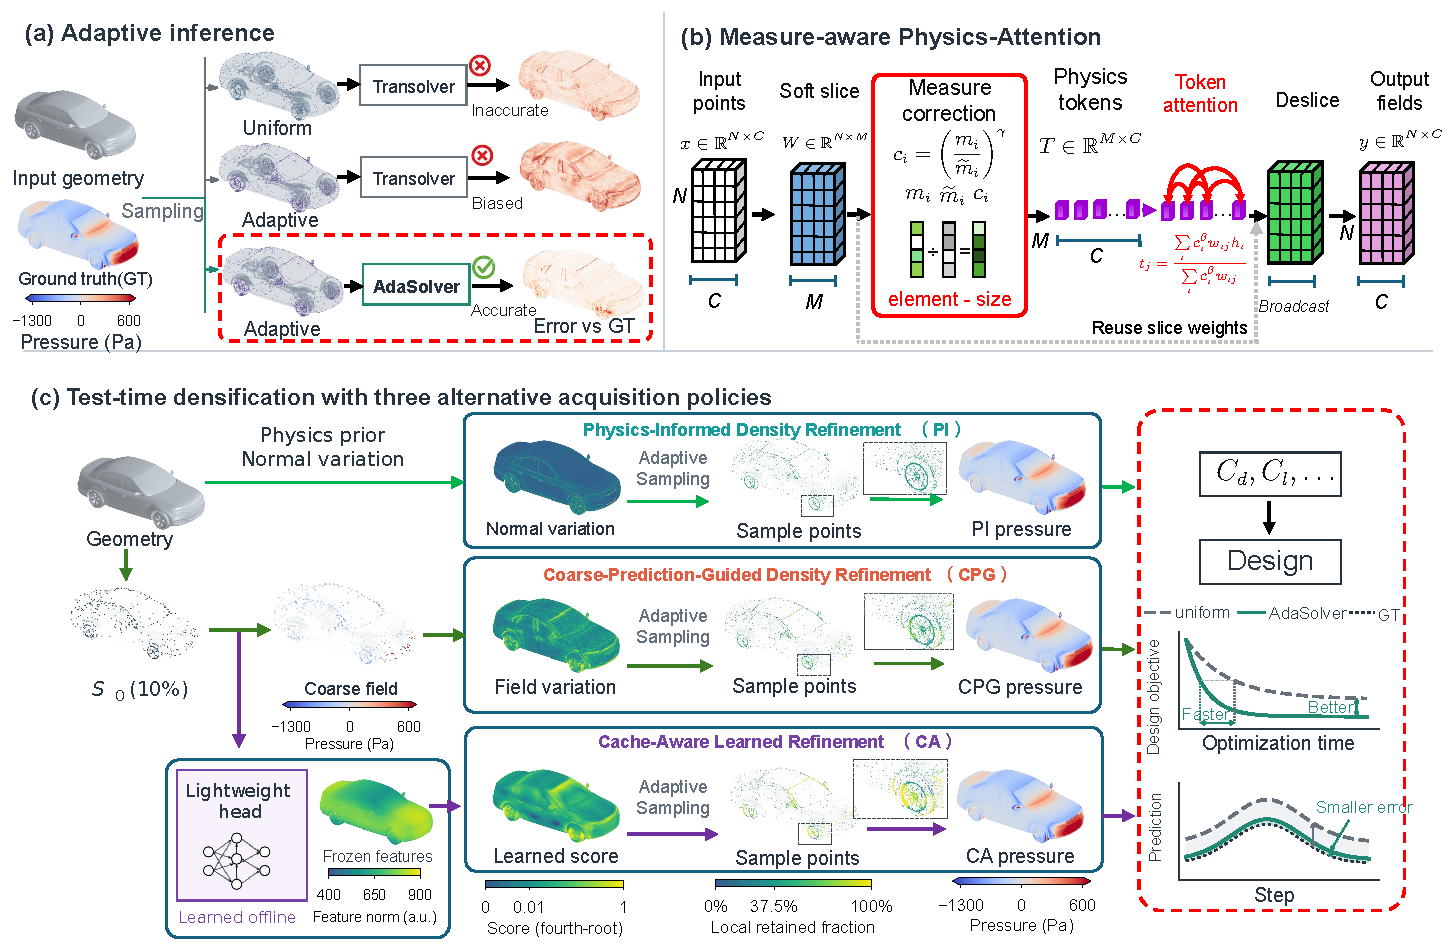
\includegraphics[width=\linewidth]{review_assets/baseline/d4021228aa183f7d5f7912124d17d3f69f8930b9/figures/fig1_overview.pdf}
%DIFDELCMD <     %%%
\DIFdelendFL \DIFaddbeginFL 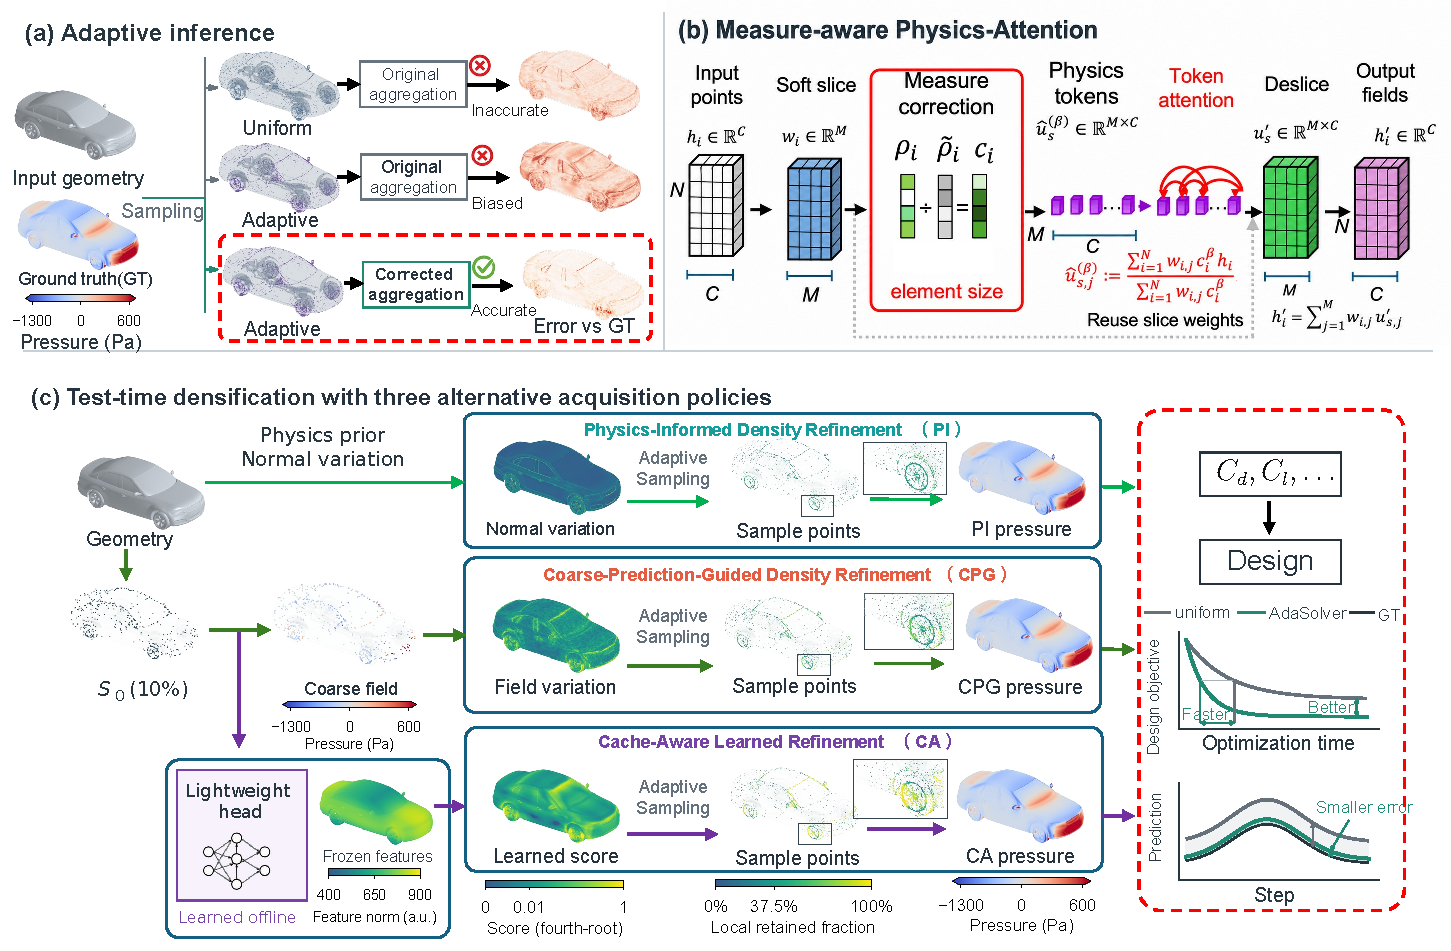
\includegraphics[width=\linewidth]{figures/fig1_overview.pdf}
    \DIFaddendFL \caption{\textbf{AdaSolver overview.} (a) Adaptive inference with \DIFdelbeginFL \DIFdelFL{measure correction}\DIFdelendFL \DIFaddbeginFL \DIFaddFL{original and corrected aggregation}\DIFaddendFL . (b) \DIFdelbeginFL \DIFdelFL{Corrected }\DIFdelendFL \DIFaddbeginFL \DIFaddFL{Measure-aware Physics-Attention with corrected }\DIFaddendFL aggregation, token attention, and deslicing. (c) Geometry priors, coarse \DIFdelbeginFL \DIFdelFL{predictions}\DIFdelendFL \DIFaddbeginFL \DIFaddFL{field variation}\DIFaddendFL , and \DIFdelbeginFL \DIFdelFL{a lightweight head on frozen
    features provide alternative refinement signals. The frozen operator evaluates
    the selected points and supplies aerodynamic quantities }\DIFdelendFL \DIFaddbeginFL \DIFaddFL{learned scores guide adaptive sampling }\DIFaddendFL for \DIFaddbeginFL \DIFaddFL{field prediction and }\DIFaddendFL design. The rightmost \DIFdelbeginFL \DIFdelFL{curves illustrate the }\DIFdelendFL design \DIFdelbeginFL \DIFdelFL{objectives schematically}\DIFdelendFL \DIFaddbeginFL \DIFaddFL{curves are schematic}\DIFaddendFL .}
    \label{fig:adasolver_overview}
\end{figure}


We summarize our contributions as follows: (i) to our knowledge, we provide the first systematic exploration of adaptive spatial sampling as a new axis of test-time scaling for neural operators, revealing sampling-measure shift as a fundamental challenge when reallocating spatial computation at inference; (ii) we introduce AdaSolver, which enables measure-consistent test-time sampling and supports diverse scaling strategies based on physics and geometry priors, coarse predictions, and learned refinement signals; and (iii) we demonstrate consistent improvements in the accuracy--compute trade-off across five standard PDE benchmarks and three industrial aerodynamic tasks, and further show that AdaSolver accelerates surrogate-based airfoil and wing optimization while achieving comparable or improved CFD-validated aerodynamic performance.

\section{Related Work}
\paragraph{Neural operators on irregular geometries.}
Fourier neural operators learn resolution-transferable spectral mappings on
regular grids, while Geo-FNO extends them to general geometries through learned
coordinate deformations \citep{li2021fno,li2023geofno}. GINO couples integral
operators with a latent regular grid, and NUNO partitions non-uniform
observations to reduce interpolation and computational costs
\citep{li2023gino,liu2023nuno}. Transformer-based operators instead compress
large point sets into latent representations before global interaction, as in
GNOT, UPT, and Transolver \citep{hao2023gnot,alkin2024upt,wu2024transolver}.
Transolver++ and Transolver-3 further scale this design to million-scale and
industrial-scale geometries \citep{luo2025transolverpp,zhou2026transolver3}.
These methods establish strong compatibility with irregular inputs. Our focus is complementary: we actively change the \emph{local} sampling density at inference and ask whether the model can preserve operator consistency while maintaining or even improving predictive performance.
\vspace{-1em}
\paragraph{Discretization-consistent operator learning.}
Extending finite neural architectures to function spaces requires discrete
reductions to converge to fixed continuous integrals as the discretization
changes \citep{berner2026functionspaces}. Monte Carlo convolution corrects
non-uniform point-cloud sampling with inverse-density weights, while QuadConv
evaluates continuous kernels using quadrature on irregular PDE data
\citep{hermosilla2018montecarlo,doherty2024quadconv}. Related formulations
construct discretization-invariant maps between neural fields and
quadrature-aware normalization statistics \citep{wang2022din,kim2026quadnorm}.
Nevertheless, resolution-independent parameters alone do not prevent errors
under a mismatch between training and evaluation discretizations
\citep{gao2025discretization}. We adopt the same function-space principle for
latent point aggregation, but use it to support a deliberate inference-time
change of sampling density rather than only passive resolution transfer.
\vspace{-1em}
\paragraph{Adaptive meshes and test-time refinement.}
Adaptive discretization concentrates resolution where numerical error is expected to be large, and learned methods predict mesh refinement or node relocation for numerical solvers \citep{huang2021meshgeneration,obiols2023adarnet,rowbottom2024gadaptivity}. Test-time compute has also been increased through iterative refinement, adaptive tokenization, and neural-operator composition \citep{lippe2023pderefiner,jenkins2026atca,wang2026adaptivetokenization,serrano2026splitting}. These methods determine where or how inference computation is allocated. AdaSolver instead addresses the operator-level challenge of changing spatial sampling density while preserving the reference operator.
\vspace{-2em}
\section{Method}
\DIFaddbegin \subsection{\DIFadd{Transolver Preliminaries}}
\label{sec:transolver_preliminaries}
\DIFaddend 

\DIFdelbegin \subsection{\DIFdel{Transolver as an Integral Operator}}
%DIFAUXCMD
\addtocounter{subsection}{-1}%DIFAUXCMD
%DIFDELCMD < 

%DIFDELCMD < %%%
\DIFdelend \DIFaddbegin \paragraph{\DIFadd{Revisiting Transolver.}}
\DIFaddend Transolver~\citep{wu2024transolver} \DIFdelbegin \DIFdel{approximates continuous integral operators through }\DIFdelend \DIFaddbegin \DIFadd{is a Transformer with
}\DIFaddend Physics-Attention\DIFdelbegin \DIFdel{. Let $\Omega$ denote the physical domain, and let $\rho$ denote the sampling measure induced by the chosen grid or mesh discretization policy. A discretized example consists of pointwise samples
$\{(x_i,a_i)\}_{i=1}^{N}\mapsto\{u_i\}_{i=1}^{N}$, where $x_i\sim\rho$, $a_i=a(x_i)$ is the input field, and $u_i=u(x_i)$ is the output field.
A neural operator learns an operator $\mathcal{G}:a\mapsto u$ with a parameterized network $\mathcal{G}_{\theta}$}\DIFdelend \DIFaddbegin \DIFadd{. Given mesh coordinates $x_i\in\Omega$ and input
conditions $a_i=a(x_i)$, it embeds $\{(x_i,a_i)\}_{i=1}^{N}$ into point
features. These pass through $L$ Transformer blocks, each comprising
Physics-Attention and a pointwise feed-forward network, with layer
normalization and residual connections. A final pointwise projection
produces the predicted physical field $\{\widehat u_i\}_{i=1}^{N}$}\DIFaddend .

\DIFaddbegin \DIFadd{Within one }\DIFaddend Physics-Attention \DIFdelbegin \DIFdel{projects point features into $M$ slice weights, applies attention to the resulting latent physical states, and broadcasts the updated states back to the points. Let $h_i\in\mathbb{R}^{C}$ denote the }\DIFdelend \DIFaddbegin \DIFadd{head, let $h_i\in\mathbb{R}^{C}$ denote a
point feature. The $N$ points are softly assigned to $M\ll N$ learned
slices: $C$ is the feature dimension, whereas $M$ is the slice count.
A slice is a learned soft group of points, with membership weights
}\begin{equation}
    \DIFadd{w_i=\operatorname{Softmax}\!\left(
        \frac{\operatorname{Linear}(h_i)}{\tau_0}\right)
    \in\mathbb{R}^{M},
    \qquad \sum_{j=1}^{M}w_{i,j}=1.
    \label{eq:transolver_slice_weights}
}\end{equation}
\DIFadd{Here, $w_{i,j}$ assigns point $i$ to slice $j$, and $\tau_0>0$ is a
temperature. Each slice is summarized by a }\DIFaddend $C$-dimensional \DIFdelbegin \DIFdel{feature embedding of $(x_i,a_i)$. The slice weights are
}\begin{displaymath}
    \DIFdel{w_i
    = \operatorname{Softmax}\!\left(\frac{\operatorname{Linear}(h_i)}{\tau_0}\right)
    \in\mathbb{R}^{M},
    \qquad
    \sum_{j=1}^{M}w_{i,j}=1,
    \relax{}
}\end{displaymath}%DIFAUXCMD
\DIFdelend \DIFaddbegin \DIFadd{token:
}\begin{equation}
    \DIFadd{u_{s,j}^{(N)}
    =\frac{\sum_{i=1}^{N}w_{i,j}h_i}{\sum_{i=1}^{N}w_{i,j}}
    \in\mathbb{R}^{C},\qquad j=1,\ldots,M.
    \label{eq:transolver_physics_state}
}\end{equation}
\DIFadd{The tag $s$ denotes slice space, while $j$ indexes a slice. With learned
query, key, and value projections $q_j=q(u_{s,j}^{(N)})$,
$k_j=k(u_{s,j}^{(N)})$, and $v_j=v(u_{s,j}^{(N)})$, attention updates
these tokens and deslicing broadcasts them back with the same weights:
}\begin{equation}
    \DIFadd{u_{s,j}'
    =\sum_{t=1}^{M}
      \frac{\exp(q_j^{\top}k_t/\tau)}{\sum_{p=1}^{M}\exp(q_j^{\top}k_p/\tau)}v_t,
    \qquad
    h_i'=\sum_{j=1}^{M}w_{i,j}u_{s,j}',
    \label{eq:transolver_state_attention}
}\end{equation}\DIFaddend 
where \DIFdelbegin \DIFdel{$\tau_0$ is the temperature. The corresponding physics token is a normalized weighted average
}\begin{displaymath}
    \DIFdel{u_{s,j}^{(N)}
    = \frac{\frac{1}{N}\sum_{i=1}^{N}w_{i,j}h_i}{\frac{1}{N}\sum_{i=1}^{N}w_{i,j}}
    \xrightarrow[N\to\infty]{}
    u_{s,j}^{\rho}
    = \frac{\int_{\Omega}w_j(x)h(x)\,\mathrm{d}\rho(x)}{\int_{\Omega}w_j(x)\,\mathrm{d}\rho(x)}.
    \relax{}
}\end{displaymath}%DIFAUXCMD
\DIFdelend \DIFaddbegin \DIFadd{$\tau>0$ is the attention temperature.
}

\paragraph{\DIFadd{Transolver as an Integral Operator.}}
\DIFadd{We now interpret these discrete operations as integral approximations.
Let $\rho$ be the reference spatial sampling measure, $\Omega_s$ a
continuous domain indexing latent slices, and $\xi_s,\xi_s'\in\Omega_s$
key and query slice coordinates. The assignment density $w(x,\xi_s)\geq0$
is normalized over $\Omega_s$; discrete memberships represent its slice
quadrature weights. Writing $w_j(x):=w(x,\xi_{s,j})$, the aggregation in
\mbox{%DIFAUXCMD
\eqref{eq:transolver_physics_state} }\hspace{0pt}%DIFAUXCMD
approximates
}\begin{equation}
    \DIFadd{u_{s,j}^{(N)}
    \xrightarrow[N\to\infty]{}
    u_{s,j}^{\rho}:=u_s^{\rho}(\xi_{s,j})
    =\frac{\int_{\Omega}w_j(x)h(x)\,\mathrm{d}\rho(x)}{\int_{\Omega}w_j(x)\,\mathrm{d}\rho(x)}.
    \label{eq:transolver_integral_token}
}\end{equation}\DIFaddend 
\DIFdelbegin %DIFDELCMD < 

%DIFDELCMD < %%%
\DIFdel{Writing $u_s^{(N)}=[u_{s,1}^{(N)},\ldots,u_{s,M}^{(N)}]^{\top}\in\mathbb{R}^{M\times C}$ and $q,k,v=\operatorname{Linear}(u_s^{(N)})$, the discrete state attention and its continuous integral
counterpart can be written together as
}\begin{displaymath}
    \DIFdel{\begin{aligned}
    u_{s,j}'
    &= \sum_{t=1}^{M}
      \frac{\exp\!\left(q_j^{\top}k_t/\tau\right)}{\sum_{p=1}^{M}\exp\!\left(q_j^{\top}k_p/\tau\right)}v_t
      \xrightarrow[M\to\infty]{}
      \mathcal{A}[u_s^{\rho}](\xi_s'), \\
    \mathcal{A}[u_s^{\rho}](\xi_s')
    &:= \int_{\Omega_s}
      \frac{\exp\!\left(q(u_s^{\rho}(\xi_s'))^{\top}k(u_s^{\rho}(\xi_s))/\tau\right)}{\int_{\Omega_s}\exp\!\left(q(u_s^{\rho}(\xi_s'))^{\top}k(u_s^{\rho}(\eta_s))/\tau\right)\,\mathrm{d}\eta_s}
      v(u_s^{\rho}(\xi_s))\,\mathrm{d}\xi_s .
    \end{aligned}
    \relax{}
}\end{displaymath}%DIFAUXCMD
\DIFdelend \DIFaddbegin \DIFadd{This spatial limit assumes independent samples from $\rho$, integrability,
and positive denominators. Likewise, token attention in
\mbox{%DIFAUXCMD
\eqref{eq:transolver_state_attention} }\hspace{0pt}%DIFAUXCMD
approximates the normalized integral
}\begin{equation}
    \DIFadd{\begin{aligned}
    u_{s,j}'&\xrightarrow[M\to\infty]{}
        \mathcal{A}[u_s^{\rho}](\xi_s'),\qquad \xi_s'=\xi_{s,j},\\
    \mathcal{A}[u_s^{\rho}](\xi_s')
    &:=\int_{\Omega_s}
      \frac{\exp\!\left(q(u_s^{\rho}(\xi_s'))^{\top}k(u_s^{\rho}(\xi_s))/\tau\right)}{\int_{\Omega_s}\exp\!\left(q(u_s^{\rho}(\xi_s'))^{\top}k(u_s^{\rho}(\eta_s))/\tau\right)\,\mathrm{d}\eta_s}
      v(u_s^{\rho}(\xi_s))\,\mathrm{d}\xi_s .
    \end{aligned}
    \label{eq:transolver_integral_attention}
}\end{equation}\DIFaddend 
\DIFdelbegin \DIFdel{where $u_s^{\rho}(\xi_s)$ is the continuous physics-token field on the slice domain$\Omega_s$, $\xi_s'$ is a query location, and $\tau$ is the attention temperature. Finally, the updated tokens are mapped back to the point space through the slice weights, }\begin{displaymath}
    \DIFdel{h_i' = \sum_{j=1}^{M}w_{i,j}u_{s,j}',
    \qquad i=1,\ldots,N.
    \relax{}
}\end{displaymath}%DIFAUXCMD
\DIFdelend \DIFaddbegin \DIFadd{Here, $M\to\infty$ describes uniform quadrature of a fixed, bounded
continuous token field on a compact slice domain; the implemented network
uses fixed $M$. Deslicing in \mbox{%DIFAUXCMD
\eqref{eq:transolver_state_attention} }\hspace{0pt}%DIFAUXCMD
then
completes the operator, under the unit-Jacobian specialization:
}\begin{equation}
    \DIFadd{h_i'\;\approx\;\mathcal{T}[u_s^{\rho}](x_i)
    :=\int_{\Omega_s}w(x_i,\xi_s')
        \mathcal{A}[u_s^{\rho}](\xi_s')\,\mathrm{d}\xi_s'.
    \label{eq:transolver_deslice}
}\end{equation}\DIFaddend 
Thus, Physics-Attention \DIFdelbegin \DIFdel{replaces the $N\times N$ point interaction with operations of complexity $\mathcal{O}(NMC+M^2C)$ for $M\ll N$. During training, the input samples used by $\mathcal{G}_{\theta}$ are typically generated according to the prescribed measure $\rho$}\DIFdelend \DIFaddbegin \DIFadd{approximates an integral operator through
aggregation, token attention, and deslicing. Appendix~\ref{app:attention_bias}
gives the general Jacobian-weighted form used in
Section~\ref{sec:density_consistent_transolver}}\DIFaddend .


\subsection{Sampling-Density-Consistent Transolver}
\label{sec:density_consistent_transolver}

Transolver is trained on point sets drawn from a prescribed sampling measure \(\rho\), induced by the discretization used to generate the training data, such as a uniform grid or a refined mesh. At inference time, we may instead sample from a different measure $\widetilde{\rho}$ to obtain a different spatial description of the same physical domain. For example, aerodynamic geometries may be sampled more densely near surfaces or flow-sensitive regions and more sparsely in smooth regions. However, changing the sampling measure alters the Monte Carlo aggregation in Transolver and therefore changes its limiting operator.

Let $\lambda=\mathrm{d}\widetilde{\rho}/\mathrm{d}\rho>0$ denote the density ratio. For a slice location $\xi_s\in\Omega_s$, define the slice-weighted probability measure
\begin{equation}
    \mathrm{d}\pi_{\xi_s}(x)
    :=\frac{w(x,\xi_s)}{\int_{\Omega}w(y,\xi_s)\,\mathrm{d}\rho(y)}\,\mathrm{d}\rho(x).
    \label{eq:main_slice_measure}
\end{equation}

\begin{proposition}[Physics-token bias under a sampling-density shift]
\label{prop:main_physics_token_bias}
For each $\xi_s\in\Omega_s$, the reference and shifted physics tokens satisfy
\begin{equation}
    u_s^{\widetilde{\rho}}(\xi_s)-u_s^{\rho}(\xi_s)
    =\frac{\operatorname{Cov}_{\pi_{\xi_s}}(\lambda,h)}{\mathbb{E}_{\pi_{\xi_s}}[\lambda]}.
    \label{eq:main_physics_token_bias}
\end{equation}
Moreover, if $\mathcal{P}_{\xi_s}^{\mu}h:=u_s^{\mu}(\xi_s)$ denotes the tokenization map under a sampling measure $\mu$, then
\begin{equation}
    \left\|\mathcal{P}_{\xi_s}^{\widetilde{\rho}}
    -\mathcal{P}_{\xi_s}^{\rho}\right\|_{\mathrm{op}}
    =\frac{\sqrt{\operatorname{Var}_{\pi_{\xi_s}}(\lambda)}}{\mathbb{E}_{\pi_{\xi_s}}[\lambda]}.
    \label{eq:main_token_operator_bias}
\end{equation}
\end{proposition}

Let $\mathcal{T}$ denote the continuous Physics-Attention operator and define $\mathcal{G}_{\mu}(h):=\mathcal{T}[u_s^{\mu}]$. Write $\delta_s:=u_s^{\widetilde{\rho}}-u_s^{\rho}$ and let $R_{\delta_s}:=\alpha_{u_s^{\widetilde{\rho}}}/\alpha_{u_s^{\rho}}$ be the ratio between the shifted and reference attention kernels.

\begin{theorem}[Propagation through continuous Physics-Attention]
\label{thm:main_physics_attention_bias}
The sampling-density bias propagates to the Physics-Attention output as
\begin{align}
    \mathcal{G}_{\widetilde{\rho}}(h)(x)-\mathcal{G}_{\rho}(h)(x)
    ={}&\int_{\Omega_s}w(x,\xi_s')
    \int_{\Omega_s}\alpha_{u_s^{\rho}}(\xi_s',\xi_s)
    \Big[(R_{\delta_s}(\xi_s',\xi_s)-1)W_vu_s^{\rho}(\xi_s)
    \nonumber\\
    &\hspace{19mm}+R_{\delta_s}(\xi_s',\xi_s)W_v\delta_s(\xi_s)\Big]
    J_g(\xi_s)\,\mathrm{d}\xi_s\,\mathrm{d}\xi_s'.
    \label{eq:main_physics_attention_bias}
\end{align}
Here $\alpha_{u_s^{\rho}}$ is the reference attention kernel, $W_v$ is the value projection, and $J_g$ is the physical-to-slice Jacobian. The two terms respectively describe the redistribution of attention weights and the propagation of shifted value tokens.
\end{theorem}

The complete conditions and proofs of Proposition~\ref{prop:main_physics_token_bias} and Theorem~\ref{thm:main_physics_attention_bias} are given in Appendix~\ref{app:measure_shift_bias}.

These results identify the point-to-slice aggregation as the source of the sampling-density bias. The slice assignment $w_{i,j}$ is computed independently at each point, attention is subsequently applied among a fixed number of physics tokens, and deslicing maps the updated tokens back to each point. Only the physics-token construction aggregates over the sampled points. Consequently, for $x_i\sim\widetilde{\rho}$, the original aggregation converges to
\begin{equation}
    \frac{\sum_{i=1}^{N}w_{i,j}h_i}{\sum_{i=1}^{N}w_{i,j}}
    \xrightarrow[N\to\infty]{}
    \frac{\int_{\Omega}w_j(x)h(x)\,\mathrm{d}\widetilde{\rho}(x)}{\int_{\Omega}w_j(x)\,\mathrm{d}\widetilde{\rho}(x)}
    =u_{s,j}^{\widetilde{\rho}},
    \label{eq:uncorrected_shifted_physics_token}
\end{equation}
rather than the reference token $u_{s,j}^{\rho}$ learned under $\rho$. We therefore correct the measure only when forming the physics tokens.
Let the measure-correction weight be
\begin{equation}
    c_i
    := \frac{\mathrm{d}\rho}{\mathrm{d}\widetilde{\rho}}(x_i)
    = \lambda(x_i)^{-1},
    \label{eq:main_importance_weight}
\end{equation}
which corresponds to the inverse relative inclusion density under discrete sampling.
The corrected aggregation becomes
\begin{equation}
    \widehat{u}_{s,j}^{(N)}
    :=\frac{\sum_{i=1}^{N}c_iw_{i,j}h_i}{\sum_{i=1}^{N}c_iw_{i,j}}
    \xrightarrow[N\to\infty]{}
    \frac{\int_{\Omega}w_j(x)h(x)\,\mathrm{d}\rho(x)}{\int_{\Omega}w_j(x)\,\mathrm{d}\rho(x)}
    =u_{s,j}^{\rho}.
    \label{eq:density_consistent_physics_token}
\end{equation}
Because the estimator is self-normalized, only relative density ratios are required. After the corrected physics tokens are obtained, we apply the original attention among physics tokens and the original deslice operation without further modification. For a Transolver with $L$ layers, the same correction is applied whenever layer $\ell$ forms new physics tokens from its current point features $h_i^{(\ell)}$:
\begin{equation}
    \widehat{u}_{s,j}^{(\ell)}
    =\frac{\sum_{i=1}^{N}c_iw_{i,j}^{(\ell)}h_i^{(\ell)}}{\sum_{i=1}^{N}c_iw_{i,j}^{(\ell)}},
    \qquad \ell=1,\ldots,L.
    \label{eq:layerwise_density_correction}
\end{equation}
Thus, for any admissible sampling density \(\widetilde{\rho}\), all learned projections and attention parameters remain unchanged, and only the point-to-slice aggregation is reweighted.


\subsection{Adaptive Test-Time Sampling for Transolver}
\label{sec:adaptive_test_time_sampling}

We next construct the inference-time sampling measure from geometry, a draft prediction, or intermediate backbone features.

Let $r_{\psi}:\Omega\to[0,\infty)$ be a nonnegative refinement score, where $\psi$ denotes the information used to construct it, and define
\begin{equation}
    \nu_{\psi}(x)
    :=\frac{r_{\psi}(x)}{\int_{\Omega}r_{\psi}(y)\,\mathrm{d}\rho(y)},
    \qquad
    \widetilde{\rho}_{\gamma,\psi}
    :=(1-\gamma)\rho+\gamma(\nu_{\psi}*\rho),
    \qquad \gamma\in[0,1].
    \label{eq:unified_refinement_measure}
\end{equation}
Here $\nu_{\psi}*\rho$ denotes the reweighted empirical measure induced by the refinement score. The correction used in the point-to-slice aggregation is
\begin{equation}
    c_{\gamma,\psi}(x)
    :=\frac{\mathrm{d}\rho}{\mathrm{d}\widetilde{\rho}_{\gamma,\psi}}(x)
    =\frac{1}{(1-\gamma)+\gamma\nu_{\psi}(x)}.
    \label{eq:unified_refinement_correction}
\end{equation}
We further parameterize the strength of measure correction as
\begin{equation}
    c_{\gamma,\psi}^{(\beta)}(x)
    := c_{\gamma,\psi}(x)^{\beta},
    \qquad \beta\in[0,1],
\end{equation}
where $\beta$ controls the strength of density compensation: $\beta=0$ recovers the original Transolver without correction, while larger $\beta$ increases the inverse-density reweighting. We use a fixed policy-specific $\beta$ in the main experiments and ablate it in Appendix~\ref{app:beta_ablation} with the sampled points held fixed.
\subsubsection{Physics-Informed Density Refinement}
\label{sec:physics_informed_refinement}

The first policy constructs $r_{\psi}$ from prior information about the geometry
or the physical problem. Let $s_{\mathrm{prior}}(x)\geq0$ be a problem-dependent
indicator whose large values identify regions expected to require finer resolution.
This indicator can be obtained from a known geometric feature, a numerical
refinement rule, or a physical quantity available before inference. We set
\begin{equation}
    \nu_{\mathrm{prior}}(x)
    :=\frac{s_{\mathrm{prior}}(x)}{\int_{\Omega}s_{\mathrm{prior}}(y)\,\mathrm{d}\rho(y)}
    \label{eq:prior_refinement_kernel}
\end{equation}
and use it in \eqref{eq:unified_refinement_measure} to draw the inference samples. This policy does not require a preliminary network evaluation; once the prior indicator is available, points are sampled from $\widetilde{\rho}_{\gamma,\mathrm{prior}}$ and inferred with the correction in \eqref{eq:unified_refinement_correction}.

\subsubsection{Coarse-Prediction-Guided Density Refinement}
\label{sec:coarse_prediction_refinement}

This strategy is motivated by PDE-Refiner~\citep{lippe2023pderefiner}
and ATCA~\citep{jenkins2026atca}. When no reliable prior is available,
we draw a small coarse sample $S_0$ from $\rho$ and evaluate the frozen
operator:
\begin{equation}
    \widehat{u}^{(0)}
    :=\mathcal{G}_{\theta}\!\left(a\big|_{S_0}\right),
    \qquad |S_0|\ll N,
    \label{eq:coarse_draft_prediction}
\end{equation}
where $a\big|_{S_0}$ denotes the input field restricted to $S_0$.
We then construct a nonnegative refinement score from the coarse prediction,
for example,
\begin{equation}
    s_{\mathrm{coarse}}(x)
    :=\Phi\!\left(
        \widehat{u}^{(0)}(x),
        \nabla\widehat{u}^{(0)}(x),
        \Delta\widehat{u}^{(0)}(x),
        \ldots
    \right),
    \qquad \Phi\geq0,
    \label{eq:coarse_refinement_score}
\end{equation}
where $\Phi$ denotes a task-dependent combination of coarse predictive
features. These quantities are estimated from the local discrete neighborhood
and extended to candidate locations when necessary. The resulting score is
normalized through \eqref{eq:unified_refinement_measure} to define
$\widetilde{\rho}_{\gamma,\mathrm{coarse}}$. The resulting density concentrates samples in regions that the coarse prediction
identifies as spatially informative or task-relevant.

\subsubsection{Cache-Aware Learned Refinement}
\label{sec:cache_aware_refinement}

Coarse-prediction-guided refinement requires a complete forward pass on
$S_0$ solely to estimate the sampling density. Moreover, once new samples are
introduced, the resulting change in the global physics tokens prevents most
of this coarse computation from being reused. We address both limitations with
a learned early refinement signal and a cache-aware final forward pass. Keeping the backbone frozen, we train a small refinement head
$H_\phi:\mathbb{R}^C\rightarrow\mathbb{R}_{+}$ on the first-block features
$h_i^{(1)}$ to directly predict the refinement score,
\begin{equation}
    r_{\mathrm{CA}}(x_i)
    := H_\phi\!\left(h_i^{(1)}\right).
    \label{eq:learned_refinement_score}
\end{equation}
The predicted score is then used in
\eqref{eq:unified_refinement_measure} to construct the adaptive sampling
density, avoiding a complete coarse forward pass.

Let $S_1=S_0\cup\Delta S$, where $\Delta S$ contains the newly sampled points.
For the first Physics-Attention layer, the pointwise input features
$h_i^{\mathrm{in}}$ and slice weights $w_{i,j}^{(1)}$ computed on $S_0$
remain unchanged when $\Delta S$ is added and can therefore be cached.
After the final sampling density and measure-correction weights $c_i$ are
determined, the first physics token is formed as
\begin{equation}
    \widehat{u}_{s,j}^{(1)}
    =
    \frac{
        \sum_{i\in S_0} c_i w_{i,j}^{(1)}h_i^{\mathrm{in}}
        +
        \sum_{i\in\Delta S} c_i w_{i,j}^{(1)}h_i^{\mathrm{in}}
    }{
        \sum_{i\in S_0} c_i w_{i,j}^{(1)}
        +
        \sum_{i\in\Delta S} c_i w_{i,j}^{(1)}
    } .
    \label{eq:cache_aware_aggregation}
\end{equation}
Thus, the pointwise quantities for $S_0$ are reused, while only those for
$\Delta S$ need to be newly computed. Token attention, deslicing, and later
blocks are recomputed on $S_1$, since the added samples alter the global
physics tokens. Appendix~\ref{app:density_policy_design} provides the
task-specific density constructions.

% \subsection{Distribution-Amortized Training}
% \label{sec:distribution_amortized_training}

% Using the measure-consistency property above, we extend the geometry-amortized training strategy of Transolver-3~\citep{zhou2026transolver3}, which trains on random subsets of a high-resolution mesh, to distribution-amortized training. At step $t$, we draw a point count $N_t$ from a prescribed range and choose a refinement configuration $(\gamma_t,\psi_t)$, giving
% \begin{equation}
%     \rho_t:=\widetilde{\rho}_{\gamma_t,\psi_t},
%     \qquad
%     x_i^{(t)}\sim\rho_t,\quad i=1,\ldots,N_t,
%     \qquad
%     S_t:=\{x_i^{(t)}\}_{i=1}^{N_t}.
%     \label{eq:distribution_amortized_sampling}
% \end{equation}
% The configuration $(\gamma_t,\psi_t)$ may be random or generated from a geometry- or physics-based refinement rule. We use the point-to-slice correction from \eqref{eq:unified_refinement_correction} during the forward pass and optimize
% \begin{equation}
%     \min_{\theta}\,\mathbb{E}_{t}
%     \left[
%     \ell\!\left(
%     \mathcal{G}_{\theta}\!\left(a\big|_{S_t}\right),
%     u\big|_{S_t}
%     \right)
%     \right].
%     \label{eq:distribution_amortized_objective}
% \end{equation}
% Because each corrected point-to-slice aggregation remains an estimator of the same $\rho$-based operator, changing $N_t$ and $\rho_t$ across training steps provides distributional augmentation without changing the operator target. Uniform variable-cardinality training is recovered when $\gamma_t=0$.


\section{Experiments}
\label{sec:experiments}

We evaluate AdaSolver on five standard PDE benchmarks and three industrial design prediction tasks. We further assess its efficiency in two CFD-validated geometry optimization tasks involving two-dimensional airfoils and three-dimensional wings.

\subsection{Benchmarks}
\label{sec:experiment_benchmarks}

Our evaluation spans canonical PDE problems and representative industrial applications. The standard PDE suite comprises Elasticity, Plasticity, Airfoil, Pipe~\citep{li2023geofno} and Darcy flow~\citep{li2021fno}. These public datasets are widely used to benchmark neural operators~\citep{hao2023gnot,wu2024transolver}. 
For industrial applications, we consider ShapeNet-Car~\citep{umetani2018learning} and DrivAerML~\citep{ashton2024drivaerml} for automotive aerodynamics, and SuperWing~\citep{yang2025superwing} for three-dimensional wing design. In addition to physical-field prediction errors, we evaluate the accuracy of design-relevant aerodynamic quantities, including the drag coefficient $C_D$, lift coefficient $C_L$, and drag-to-lift ratio $C_D/C_L$. We also use the learned PDE surrogates to guide shape optimization of a two-dimensional airfoil and a three-dimensional wing, assessing computational efficiency and aerodynamic prediction accuracy during optimization. Governing equations, data splits, and input--output mappings are detailed in Appendix~\ref{app:implementation_details}.


\subsection{Implementation and Evaluation}
\label{sec:experiment_implementation}

As described in \DIFdelbegin \DIFdel{\mbox{%DIFAUXCMD
\eqref{eq:transolver_physics_state} }\hspace{0pt}%DIFAUXCMD
and~\mbox{%DIFAUXCMD
\eqref{eq:transolver_state_attention}}\hspace{0pt}%DIFAUXCMD
}\DIFdelend \DIFaddbegin \DIFadd{\mbox{%DIFAUXCMD
\eqref{eq:transolver_integral_token} }\hspace{0pt}%DIFAUXCMD
and~\mbox{%DIFAUXCMD
\eqref{eq:transolver_integral_attention}}\hspace{0pt}%DIFAUXCMD
}\DIFaddend , Transolver approximates a continuous integral operator through point aggregation and attention over latent physical states. With the number of physical states fixed, varying the spatial sampling budget changes the number of point samples used to estimate the aggregation integrals. For Airfoil, Pipe, Elasticity, and Plasticity, we adopt geometry-amortized training from Transolver-3~\citep{zhou2026transolver3}. Given a full mesh of $N$ points, we draw a point count $N_t$ uniformly from $\{\operatorname{round}(0.4N),\ldots,N\}$ for each minibatch, then sample $N_t$ mesh points uniformly without replacement. Darcy uses the existing backbone trained on full meshes. The trained backbone is frozen when evaluating different sampling policies and inference budgets.

For a consistent comparison, we treat all input discretizations as unstructured meshes and evaluate sampling budgets of $37.5\%$, $50\%$, and $75\%$ of the full-mesh point count. Uniform subsampling of mesh points serves as the common baseline. We report \DIFaddbegin \DIFadd{full-field }\DIFaddend relative $L_2$ errors \DIFdelbegin \DIFdel{for physical-field predictions }\DIFdelend \DIFaddbegin \DIFadd{(Appendix~\ref{app:full_field_reconstruction}) }\DIFaddend and summarize performance across budgets using the relative area under the error--budget curve (rAUEC). Let $b_k$ denote the retained fraction of mesh points, with $(b_1,b_2,b_3)=(0.375,0.50,0.75)$, and let $E_{\mathrm{method}}(b)$ and $E_{\mathrm{uniform}}(b)$ denote mean test errors for a given sampling seed. Using trapezoidal integration, we compute
\begin{equation}
    \mathrm{rAUEC}
    :=
    \frac{\sum_{k=1}^{2}(b_{k+1}-b_k)
          \bigl[E_{\mathrm{method}}(b_k)+E_{\mathrm{method}}(b_{k+1})\bigr]}{\sum_{k=1}^{2}(b_{k+1}-b_k)
          \bigl[E_{\mathrm{uniform}}(b_k)+E_{\mathrm{uniform}}(b_{k+1})\bigr]}.
    \label{eq:rauec}
\end{equation}
Lower rAUEC is better, with \textbf{uniform sampling normalized to $1$}.
% Airfoil uses the same 110 cases with reference $C_L>0.02$ for field and $C_D/C_L$ evaluation, with metric-specific sampling policies and absolute error for $C_D/C_L$. Elasticity uses 200 independent holdout cases.

% For industrial benchmarks, ShapeNet-Car combines full-cloud velocity relative $L_2$ with half the surface-pressure relative $L_2$ error. DrivAerML uses surface-pressure relative $L_2$, and SuperWing uses joint relative $L_2$ on the dataset-scaled pressure and skin-friction channels. The aerodynamic metrics are relative errors in $C_D$ for the car datasets and $C_D/C_L$ for SuperWing, with sampling policies selected separately for each metric. ShapeNet-Car and DrivAerML use 100 and 50 test geometries, respectively. SuperWing uses 2,871 cases for field evaluation and a fixed 2,563-case subset for $C_D/C_L$, selected by a calibration-derived lift-magnitude cutoff of approximately $0.071$.

\subsection{Main Results}
\label{sec:main_results}

\paragraph{Standard Benchmarks.}
Table~\ref{tab:standard_benchmarks} compares physics-informed density
refinement (PI), coarse-prediction-guided density refinement (CPG), and
cache-aware learned refinement (CA) against uniform subsampling across five
standard PDE benchmarks. Overall, adaptive test-time sampling improves the
error--budget trade-off, demonstrating that sampling density provides a
controllable axis for test-time computation. CPG generally outperforms PI,
suggesting that solution-dependent variation can provide more informative
refinement cues than geometry or prescribed heuristics alone. CA performs
comparably to CPG on several tasks, showing that such solution-aware signals
can be recovered from intermediate features without requiring a complete
coarse prediction. The distinction is particularly clear on Darcy: despite its
regular Cartesian grid, PI offers little improvement over uniform sampling,
whereas CPG and CA substantially reduce rAUEC. This result indicates that the
benefit of adaptive sampling is not limited to geometric complexity, but also
depends on how well the sampling density captures localized structure in the
solution.

\begin{table}[!htbp]
    \centering
    \small
    \caption{rAUEC ($\downarrow$) on standard PDE benchmarks.  Means appear above standard deviations ($n=3$ \DIFaddbeginFL \DIFaddFL{sampling seeds}\DIFaddendFL ). Best and second-best means are \textbf{bold} and \underline{underlined}, respectively.}
    \label{tab:standard_benchmarks}
    \setlength{\tabcolsep}{3pt}
    \renewcommand{\arraystretch}{1.12}
    \begin{tabular*}{\textwidth}{@{\extracolsep{\fill}}lcccccc@{}}
        \toprule
        & \multicolumn{2}{c}{Airfoil2D} & Pipe & Darcy & Elasticity & Plasticity \\
        \cmidrule(lr){2-3}
        Method & Field & $C_D/C_L$ & Field & Field & Field & Field \\
        \midrule
        PI & $\begin{gathered}0.6166\\[-2pt]\pm 0.0197\end{gathered}$ & $\begin{gathered}\mathbf{0.2174}\\[-2pt]\pm 0.1688\end{gathered}$ & $\begin{gathered}0.8711\\[-2pt]\pm 0.0061\end{gathered}$ & $\begin{gathered}0.9965\\[-2pt]\pm 0.0177\end{gathered}$ & \DIFdelbeginFL \DIFdelFL{%
\mbox{%DIFAUXCMD
$\begin{gathered}0.7280\\[-2pt]\pm 0.0083\end{gathered}$
}%DIFAUXCMD
}\DIFdelendFL \DIFaddbeginFL \DIFaddFL{%
\mbox{%DIFAUXCMD
$\begin{gathered}0.7262\\[-2pt]\pm 0.0082\end{gathered}$
}%DIFAUXCMD
}\DIFaddendFL & $\begin{gathered}\mathbf{0.8888}\\[-2pt]\pm 0.0041\end{gathered}$ \\
        \addlinespace[3pt]
        CPG & $\begin{gathered}\underline{0.5831}\\[-2pt]\pm 0.0219\end{gathered}$ & $\begin{gathered}\underline{0.2379}\\[-2pt]\pm 0.1781\end{gathered}$ & $\begin{gathered}\mathbf{0.6719}\\[-2pt]\pm 0.0098\end{gathered}$ & $\begin{gathered}\underline{0.6419}\\[-2pt]\pm 0.0049\end{gathered}$ & $\begin{gathered}\mathbf{0.4681}\\[-2pt]\pm 0.0041\end{gathered}$ & $\begin{gathered}\underline{0.8890}\\[-2pt]\pm 0.0038\end{gathered}$ \\
        \addlinespace[3pt]
        CA & $\begin{gathered}\mathbf{0.5579}\\[-2pt]\pm 0.0139\end{gathered}$ & $\begin{gathered}0.2453\\[-2pt]\pm 0.1779\end{gathered}$ & $\begin{gathered}\underline{0.7051}\\[-2pt]\pm 0.0116\end{gathered}$ & $\begin{gathered}\mathbf{0.6400}\\[-2pt]\pm 0.0062\end{gathered}$ & $\begin{gathered}\underline{0.5469}\\[-2pt]\pm 0.0021\end{gathered}$ & $\begin{gathered}0.8897\\[-2pt]\pm 0.0049\end{gathered}$ \\
        \bottomrule
    \end{tabular*}
\end{table}


\paragraph{Industrial Applications.}
Accurate aerodynamic surrogate modeling requires both high-fidelity full-field
prediction and reliable estimation of design-relevant quantities. Table~\ref{tab:industrial_benchmarks} evaluates both aspects on
ShapeNet-Car, DrivAerML, and SuperWing. Across all three datasets, adaptive
sampling consistently improves the error--budget trade-off for both field
predictions and aerodynamic metrics. Notably, several aerodynamic quantities
match or even surpass full-mesh accuracy using only about one-third of the
points, indicating that spatial resolution can be concentrated in physically
informative regions without sacrificing global field fidelity. The qualitative
results in Figure~\ref{fig:field_comparison} support this interpretation:
adaptive policies concentrate samples around localized solution structures and
geometrically or physically sensitive regions, where the corresponding
prediction residuals are also reduced relative to uniform sampling. Together, these results show that adaptive sampling improves accuracy by concentrating test-time resolution in more informative regions. Appendix~\ref{app:beta_ablation} isolates the effect of measure correction,
followed by budget-wise error curves and full-field visualizations across all eight benchmarks.
\begin{table}[!htbp]
    \centering
    \small
    \caption{rAUEC ($\downarrow$) on industrial benchmarks. Means appear above standard deviations ($n=3$ \DIFaddbeginFL \DIFaddFL{sampling seeds}\DIFaddendFL ). Best and second-best means are \textbf{bold} and \underline{underlined}, respectively. }
    \label{tab:industrial_benchmarks}
    \setlength{\tabcolsep}{3pt}
    \renewcommand{\arraystretch}{1.12}
    \begin{tabular*}{\textwidth}{@{\extracolsep{\fill}}lcccccc@{}}
        \toprule
        & \multicolumn{2}{c}{ShapeNet-Car} & \multicolumn{2}{c}{DrivAerML} & \multicolumn{2}{c}{SuperWing} \\
        \cmidrule(lr){2-3}\cmidrule(lr){4-5}\cmidrule(lr){6-7}
        Method & Field & $C_D$ & Field & $C_D$ & Field & $C_D/C_L$ \\
        \midrule
        PI & \DIFdelbeginFL \DIFdelFL{%
\mbox{%DIFAUXCMD
$\begin{gathered}0.58952\\[-2pt]\pm 0.00180\end{gathered}$
}%DIFAUXCMD
}\DIFdelendFL \DIFaddbeginFL \DIFaddFL{%
\mbox{%DIFAUXCMD
$\begin{gathered}\mathbf{0.49792}\\[-2pt]\pm 0.00163\end{gathered}$
}%DIFAUXCMD
}\DIFaddendFL & \DIFdelbeginFL \DIFdelFL{%
\mbox{%DIFAUXCMD
$\begin{gathered}0.65606\\[-2pt]\pm 0.00168\end{gathered}$
}%DIFAUXCMD
}\DIFdelendFL \DIFaddbeginFL \DIFaddFL{%
\mbox{%DIFAUXCMD
$\begin{gathered}\mathbf{0.63346}\\[-2pt]\pm 0.00328\end{gathered}$
}%DIFAUXCMD
}\DIFaddendFL & $\begin{gathered}0.88342\\[-2pt]\pm 0.00011\end{gathered}$ & $\begin{gathered}0.92455\\[-2pt]\pm 0.00149\end{gathered}$ & $\begin{gathered}0.75640\\[-2pt]\pm 0.00079\end{gathered}$ & $\begin{gathered}0.82456\\[-2pt]\pm 0.00539\end{gathered}$ \\
        \addlinespace[3pt]
        CPG & \DIFdelbeginFL \DIFdelFL{%
\mbox{%DIFAUXCMD
$\begin{gathered}\mathbf{0.55770}\\[-2pt]\pm 0.00219\end{gathered}$
}%DIFAUXCMD
}\DIFdelendFL \DIFaddbeginFL \DIFaddFL{%
\mbox{%DIFAUXCMD
$\begin{gathered}0.50064\\[-2pt]\pm 0.00157\end{gathered}$
}%DIFAUXCMD
}\DIFaddendFL & \DIFdelbeginFL \DIFdelFL{%
\mbox{%DIFAUXCMD
$\begin{gathered}\mathbf{0.64743}\\[-2pt]\pm 0.00454\end{gathered}$
}%DIFAUXCMD
}\DIFdelendFL \DIFaddbeginFL \DIFaddFL{%
\mbox{%DIFAUXCMD
$\begin{gathered}\underline{0.63530}\\[-2pt]\pm 0.00396\end{gathered}$
}%DIFAUXCMD
}\DIFaddendFL & $\begin{gathered}\mathbf{0.82458}\\[-2pt]\pm 0.00005\end{gathered}$ & $\begin{gathered}\mathbf{0.92093}\\[-2pt]\pm 0.00148\end{gathered}$ & $\begin{gathered}\mathbf{0.67059}\\[-2pt]\pm 0.00212\end{gathered}$ & $\begin{gathered}\mathbf{0.80259}\\[-2pt]\pm 0.00761\end{gathered}$ \\
        \addlinespace[3pt]
        CA & \DIFdelbeginFL \DIFdelFL{%
\mbox{%DIFAUXCMD
$\begin{gathered}\underline{0.55774}\\[-2pt]\pm 0.00222\end{gathered}$
}%DIFAUXCMD
}\DIFdelendFL \DIFaddbeginFL \DIFaddFL{%
\mbox{%DIFAUXCMD
$\begin{gathered}\underline{0.50063}\\[-2pt]\pm 0.00159\end{gathered}$
}%DIFAUXCMD
}\DIFaddendFL & \DIFdelbeginFL \DIFdelFL{%
\mbox{%DIFAUXCMD
$\begin{gathered}\underline{0.64786}\\[-2pt]\pm 0.00404\end{gathered}$
}%DIFAUXCMD
}\DIFdelendFL \DIFaddbeginFL \DIFaddFL{%
\mbox{%DIFAUXCMD
$\begin{gathered}0.63540\\[-2pt]\pm 0.00440\end{gathered}$
}%DIFAUXCMD
}\DIFaddendFL & $\begin{gathered}\underline{0.82635}\\[-2pt]\pm 0.00019\end{gathered}$ & $\begin{gathered}\underline{0.92438}\\[-2pt]\pm 0.00153\end{gathered}$ & $\begin{gathered}\underline{0.71927}\\[-2pt]\pm 0.00211\end{gathered}$ & $\begin{gathered}\underline{0.81675}\\[-2pt]\pm 0.00700\end{gathered}$ \\
        \bottomrule
    \end{tabular*}
\end{table}


\begin{figure}[!htbp]
    \centering
    \DIFdelbeginFL %DIFDELCMD < 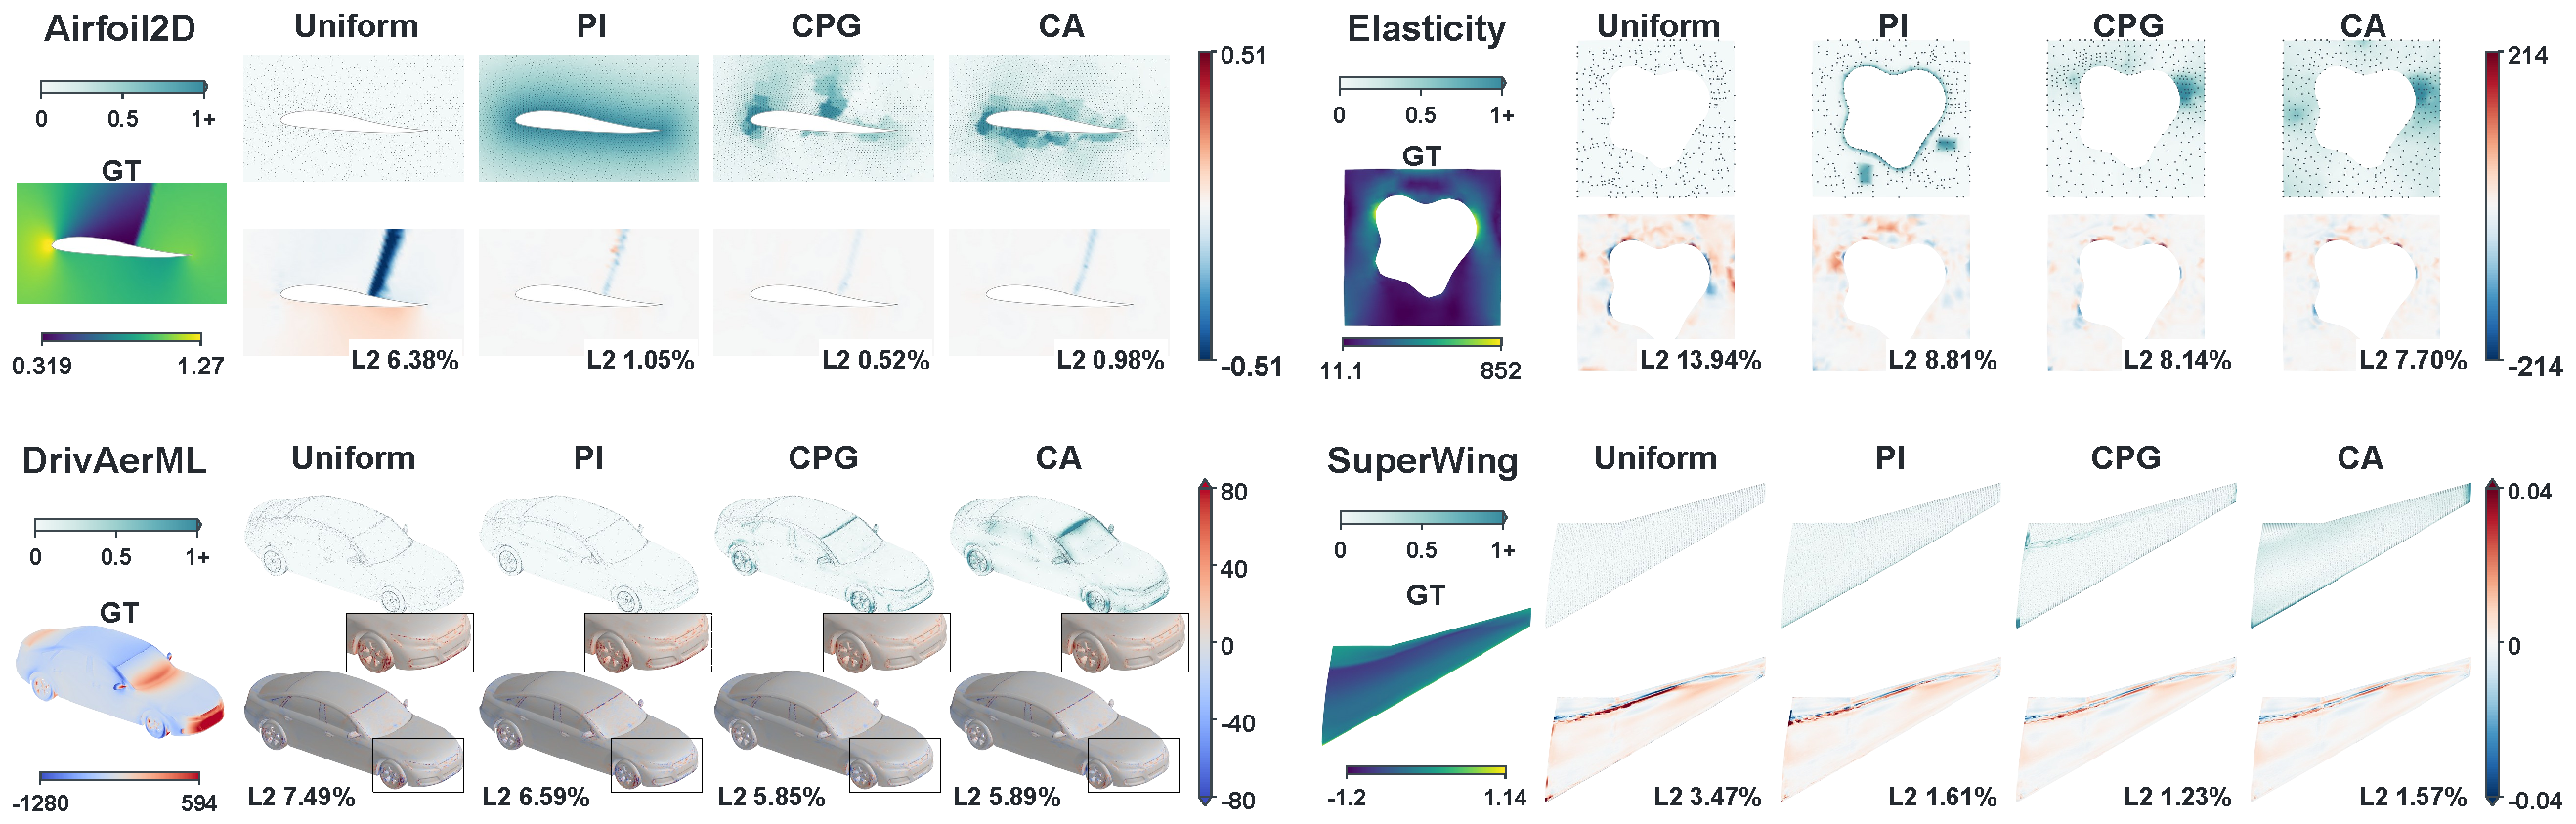
\includegraphics[width=\linewidth]{review_assets/baseline/d4021228aa183f7d5f7912124d17d3f69f8930b9/figures/fig2_field_comparison.pdf}
%DIFDELCMD <     %%%
\DIFdelendFL \DIFaddbeginFL 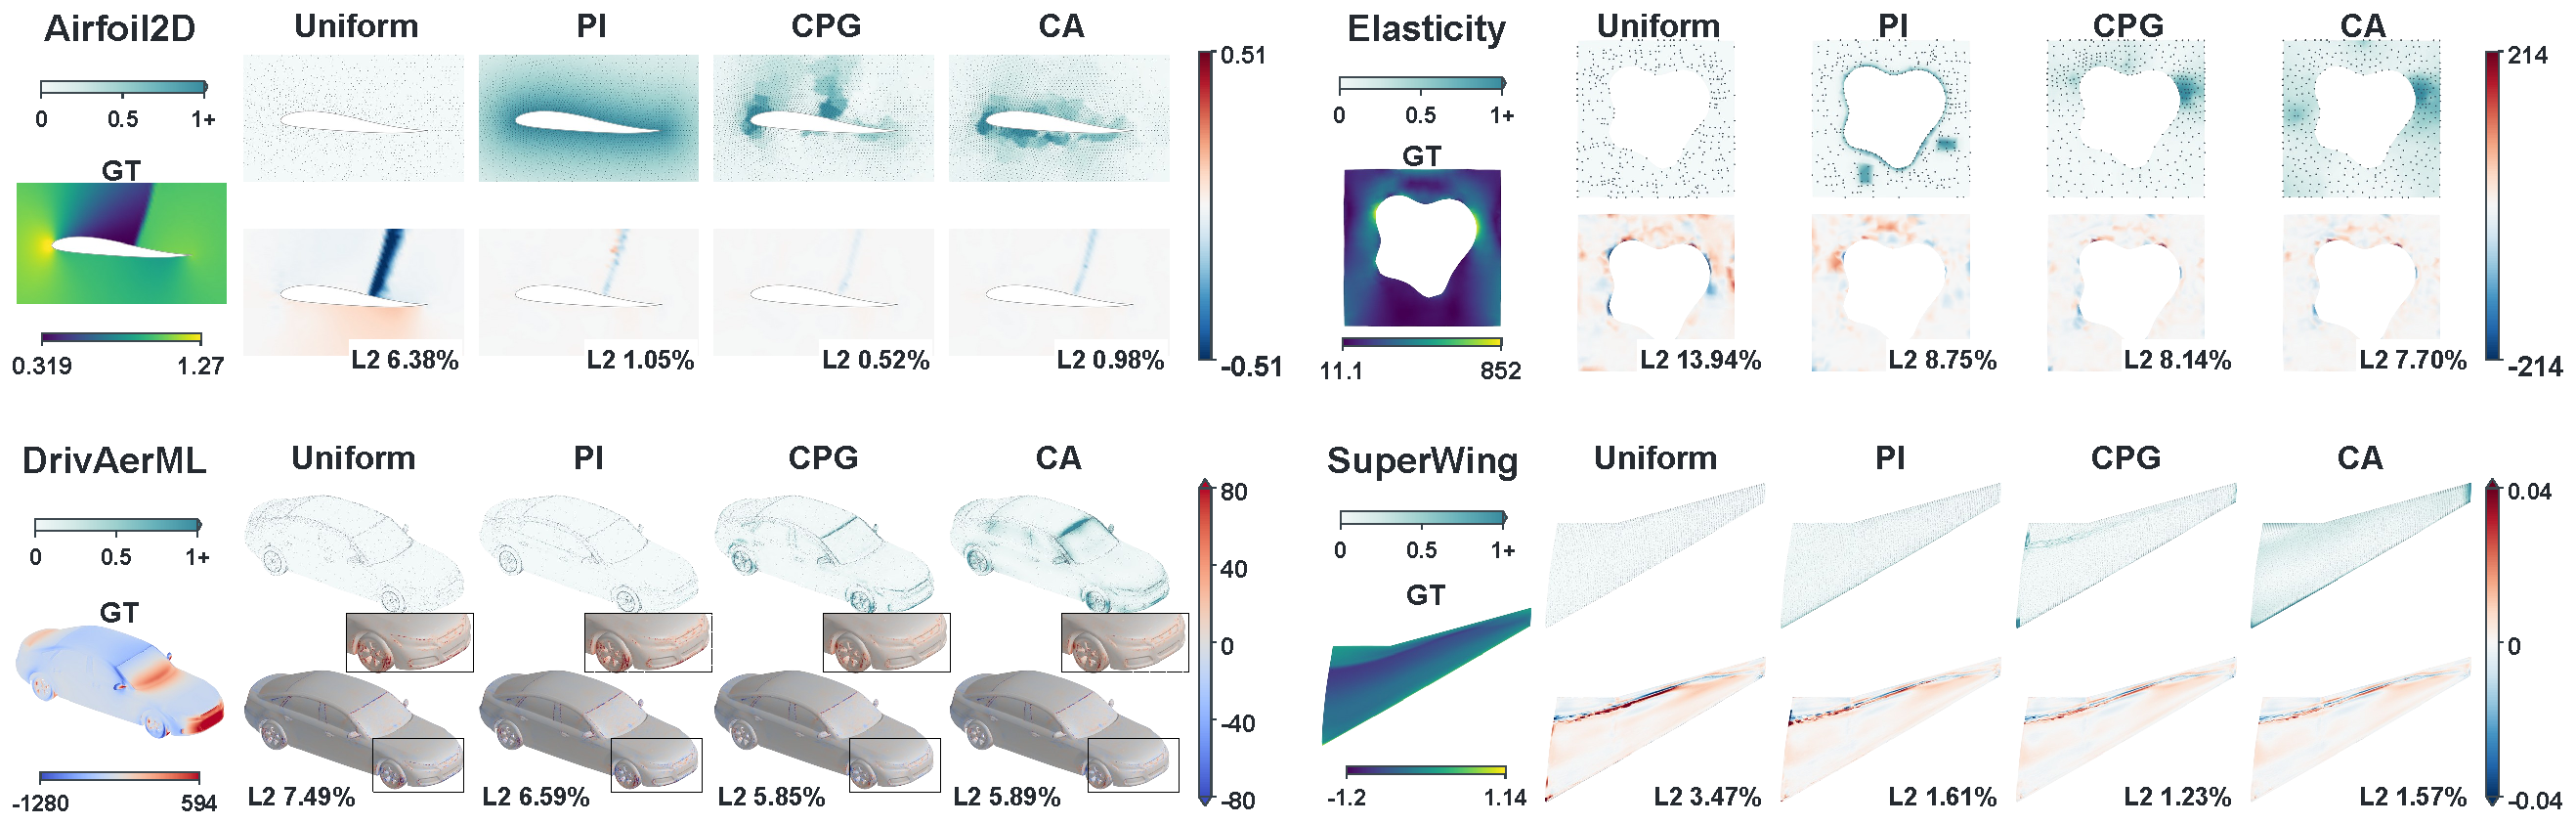
\includegraphics[width=\linewidth]{figures/fig2_field_comparison.pdf}
    \DIFaddendFL \caption{\textbf{Adaptive sampling and field prediction.}
Four test cases at a $37.5\%$ point budget. Upper rows show samples overlaid on
\DIFdelbeginFL \DIFdelFL{sampling densities}\DIFdelendFL \DIFaddbeginFL \DIFaddFL{refinement signals}\DIFaddendFL ; lower rows show signed prediction errors relative to ground
truth. Annotations report
relative $L_2$ field errors.}
    \label{fig:field_comparison}
\end{figure}
\vspace{-1em}

\subsection{Inverse Design}
\label{sec:inverse_design}

We evaluate AdaSolver in surrogate-based airfoil and wing design. The airfoil
task minimizes $(C_D/C_L)^2$, while SuperWing minimizes drag subject to a
fixed-lift target. Final designs are independently validated with CFD.
Appendix~\ref{app:inverse_design_settings} details the geometry controls,
optimization constraints, sampling schedules, and CFD settings.

\paragraph{2D Airfoil.}
We follow the airfoil inverse-design setting of Geo-FNO~\citep{li2023geofno},
parameterizing the geometry by spline-node displacements and performing
gradient-based optimization through the differentiable surrogate.
AdaSolver retains 2,113 of 11,271 points ($18.75\%$) and keeps the sampled
indices fixed after initialization. It \DIFdelbegin \DIFdel{accelerates the complete design process by $2.18\times$ }\DIFdelend \DIFaddbegin \DIFadd{reduces online optimization time from
$0.98$ to $0.44$\,s }\DIFaddend while
reaching essentially the same CFD-validated aerodynamic performance as
full-mesh optimization. It also yields a substantially more accurate surrogate
estimate of the final design, demonstrating that adaptive test-time sampling
can reduce optimization cost without compromising design quality. 
\begin{figure}[!htbp]
    \centering
    \DIFdelbeginFL %DIFDELCMD < 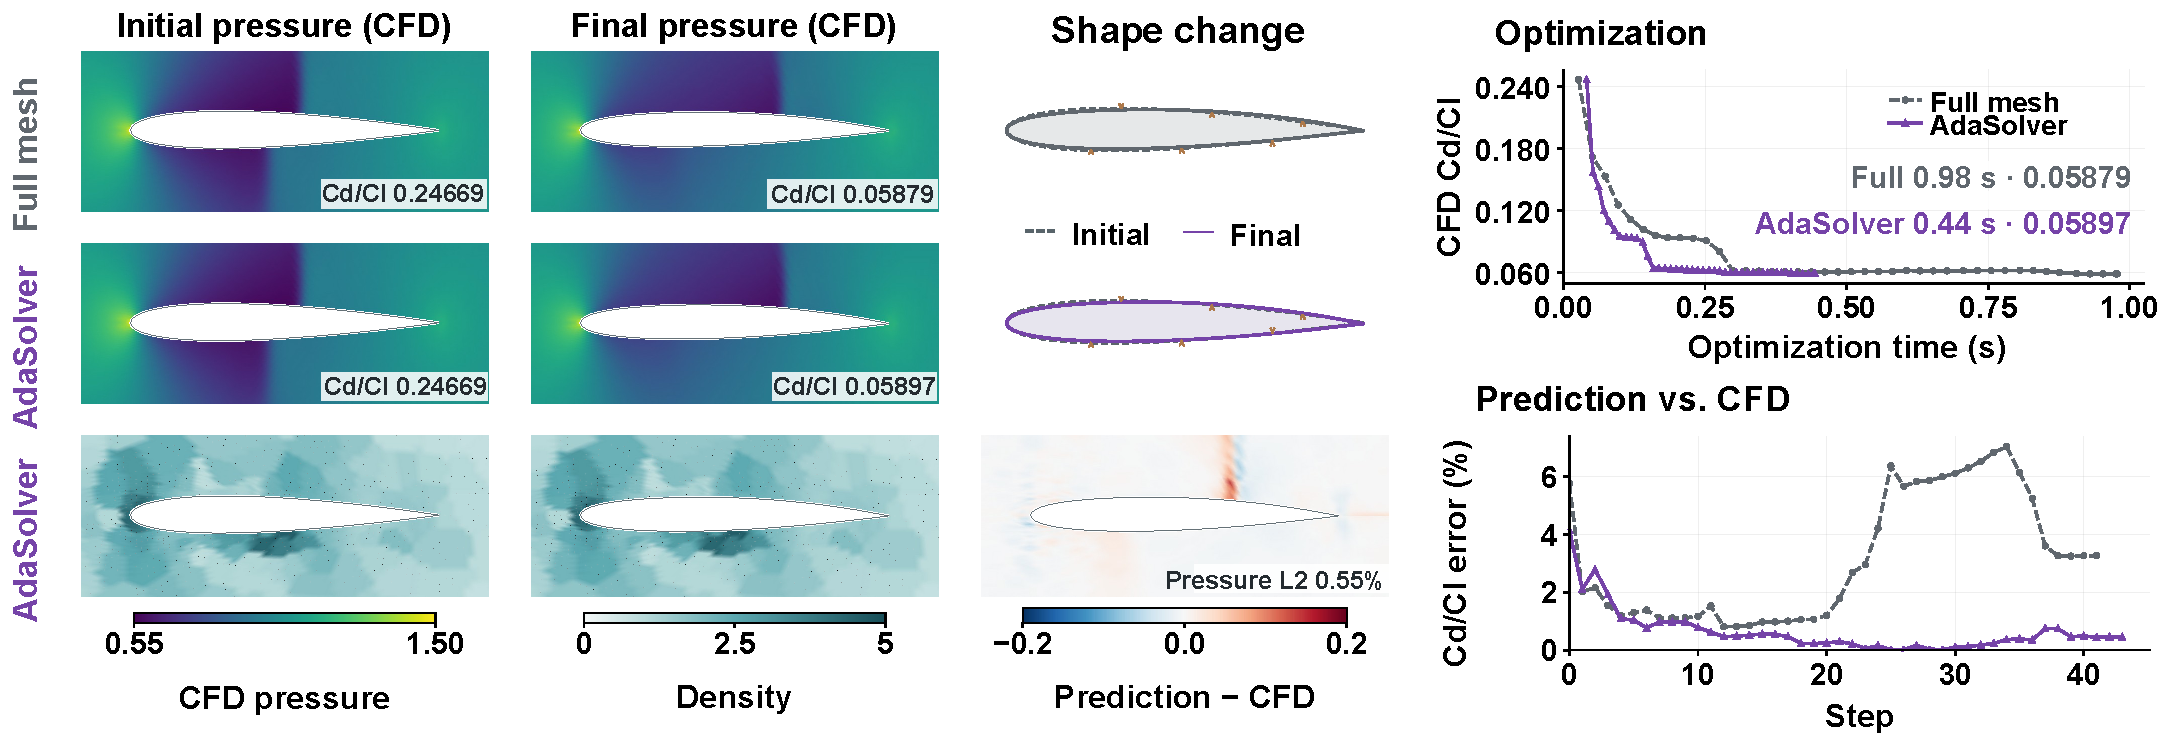
\includegraphics[width=\linewidth]{review_assets/baseline/d4021228aa183f7d5f7912124d17d3f69f8930b9/figures/fig3_airfoil_optimization.pdf}
%DIFDELCMD <     %%%
\DIFdelendFL \DIFaddbeginFL 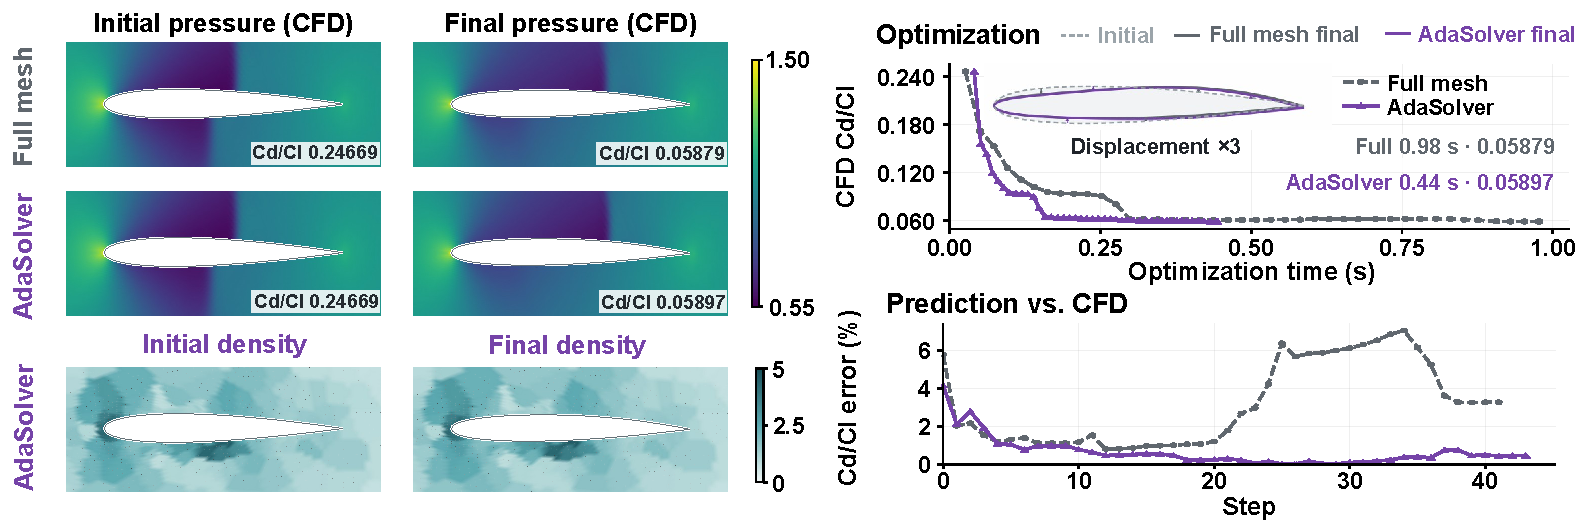
\includegraphics[width=\linewidth]{figures/fig3_airfoil_optimization.pdf}
    \DIFaddendFL \caption{\textbf{Two-dimensional airfoil optimization.} Left: initial \DIFdelbeginFL \DIFdelFL{/}\DIFdelendFL \DIFaddbeginFL \DIFaddFL{and }\DIFaddendFL final \DIFaddbeginFL \DIFaddFL{CFD }\DIFaddendFL pressure \DIFaddbeginFL \DIFaddFL{fields for Full mesh and AdaSolver}\DIFaddendFL , \DIFdelbeginFL \DIFdelFL{shape changes, }\DIFdelendFL \DIFaddbeginFL \DIFaddFL{with }\DIFaddendFL AdaSolver \DIFdelbeginFL \DIFdelFL{density
    (}\DIFdelendFL sampling \DIFdelbeginFL \DIFdelFL{weights; uniform $=1$), retained points, and pressure error}\DIFdelendFL \DIFaddbeginFL \DIFaddFL{densities}\DIFaddendFL . Right: \DIFaddbeginFL \DIFaddFL{initial and optimized shapes with displacements amplified $3\times$, }\DIFaddendFL CFD $C_D/C_L$ versus \DIFdelbeginFL \DIFdelFL{online }\DIFdelendFL optimization time\DIFdelbeginFL \DIFdelFL{;
    }\DIFdelendFL \DIFaddbeginFL \DIFaddFL{, and }\DIFaddendFL relative \DIFdelbeginFL \DIFdelFL{ratio }\DIFdelendFL \DIFaddbeginFL \DIFaddFL{$C_D/C_L$ }\DIFaddendFL prediction error \DIFaddbeginFL \DIFaddFL{against CFD }\DIFaddendFL over \DIFdelbeginFL \DIFdelFL{accepted }\DIFdelendFL \DIFaddbeginFL \DIFaddFL{optimization }\DIFaddendFL steps.}
    \label{fig:airfoil_design}
\end{figure}
\vspace{-1em}

\FloatBarrier
\paragraph{3D SuperWing.}
Figure~\ref{fig:superwing_design} compares CMA-ES~\citep{hansen2001completely}
optimization on SuperWing~\citep{yang2025superwing}, with both methods initialized
from the same geometry and flow condition. AdaSolver evaluates only $37.5\%$ of
the surface points and periodically refreshes the sampling density as the geometry
evolves. Since nearby optimization iterates typically exhibit similar geometries,
the same density can be reused across multiple steps, avoiding unnecessary
resampling overhead. AdaSolver achieves a $1.86\times$ speedup while attaining a
slightly lower CFD-validated $C_D/C_L$ than full-mesh optimization. As shown in
Figure~\ref{fig:superwing_design}, the relative prediction error also decreases
from $3.82\%$ to $3.30\%$. 
\begin{figure}[!htbp]
    \centering
    \DIFdelbeginFL %DIFDELCMD < 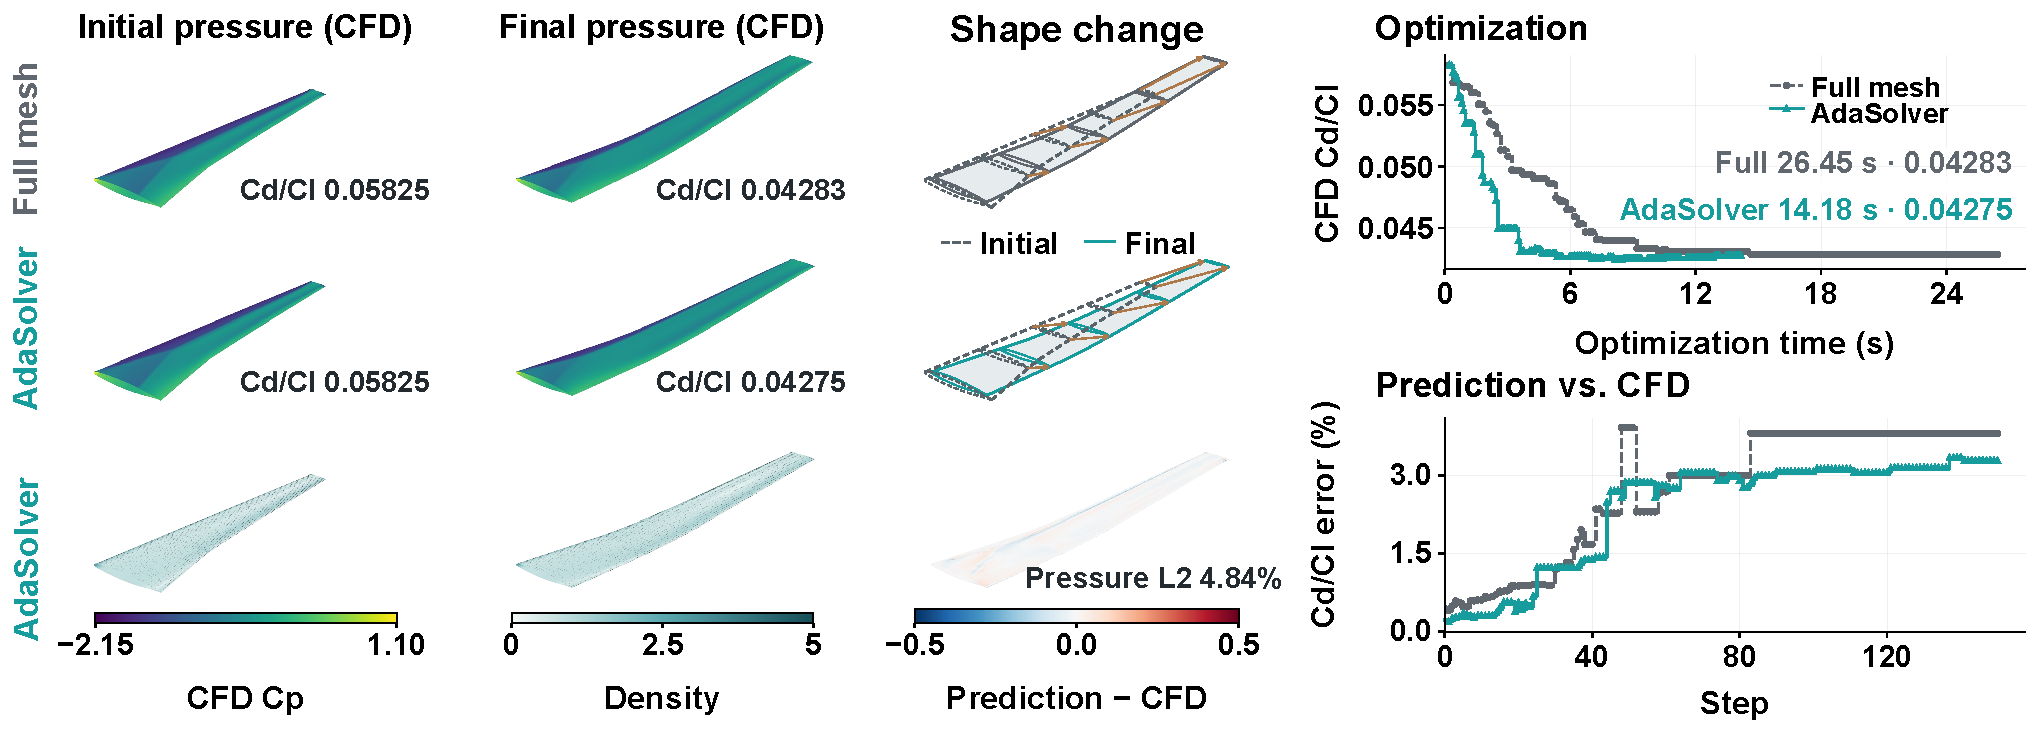
\includegraphics[width=\linewidth]{review_assets/baseline/d4021228aa183f7d5f7912124d17d3f69f8930b9/figures/fig4_superwing_optimization.pdf}
%DIFDELCMD <     %%%
\DIFdelendFL \DIFaddbeginFL 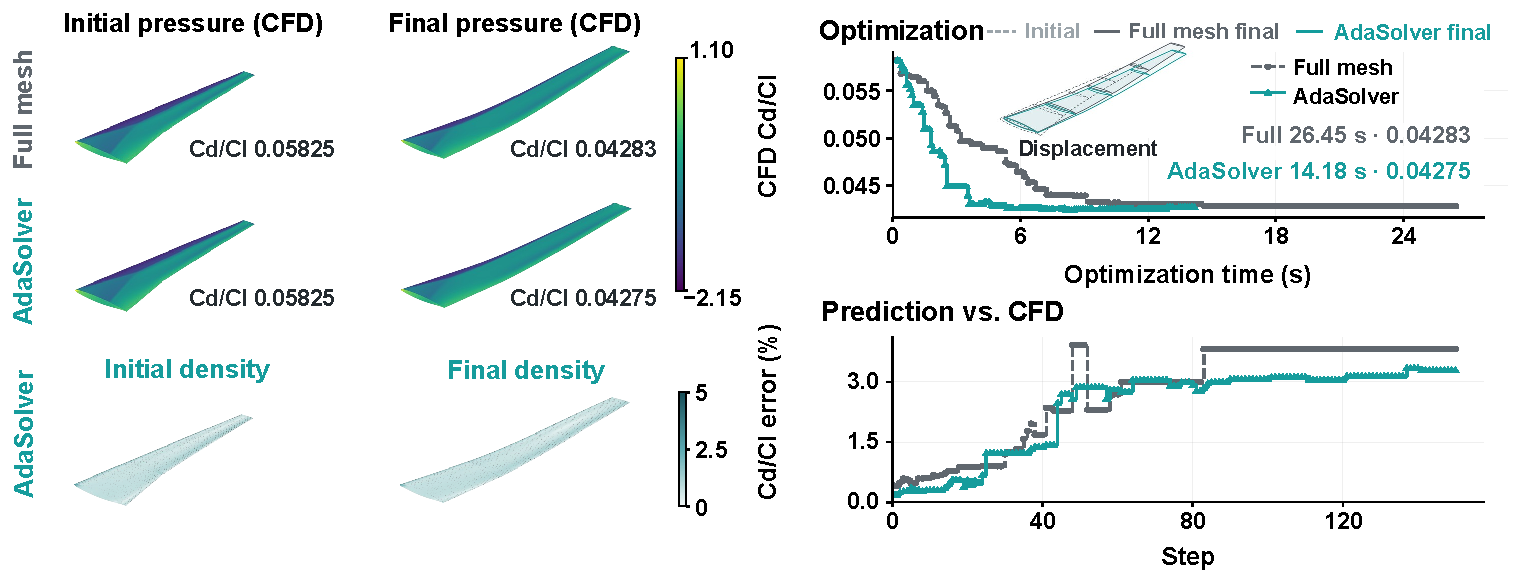
\includegraphics[width=\linewidth]{figures/fig4_superwing_optimization.pdf}
    \DIFaddendFL \caption{\textbf{SuperWing optimization.} Left: \DIFaddbeginFL \DIFaddFL{initial and final }\DIFaddendFL CFD pressure coefficients \DIFdelbeginFL \DIFdelFL{, shape changes, }\DIFdelendFL \DIFaddbeginFL \DIFaddFL{for Full mesh and }\DIFaddendFL AdaSolver\DIFdelbeginFL \DIFdelFL{density
    (normalized as in Figure~\ref{fig:airfoil_design})}\DIFdelendFL , \DIFdelbeginFL \DIFdelFL{retained points, and pressure error}\DIFdelendFL \DIFaddbeginFL \DIFaddFL{with AdaSolver sampling densities}\DIFaddendFL . Right: \DIFdelbeginFL \DIFdelFL{independently CFD-evaluated }\DIFdelendFL \DIFaddbeginFL \DIFaddFL{initial and optimized shapes, CFD }\DIFaddendFL $C_D/C_L$ versus optimization time\DIFdelbeginFL \DIFdelFL{;
    }\DIFdelendFL \DIFaddbeginFL \DIFaddFL{, and }\DIFaddendFL relative \DIFdelbeginFL \DIFdelFL{ratio }\DIFdelendFL \DIFaddbeginFL \DIFaddFL{$C_D/C_L$ }\DIFaddendFL prediction error \DIFaddbeginFL \DIFaddFL{against CFD }\DIFaddendFL over \DIFdelbeginFL \DIFdelFL{150 generations}\DIFdelendFL \DIFaddbeginFL \DIFaddFL{optimization steps}\DIFaddendFL .}
    \label{fig:superwing_design}
\end{figure}
\vspace{-2em}


\FloatBarrier
\section{Conclusion}
\label{sec:conclusion}
AdaSolver turns spatial sampling density from a fixed discretization choice into a controllable design variable at test time. By compensating for the induced measure shift, it decouples where computation is allocated from the reference operator being approximated, establishing spatial sampling as a new axis of test-time scaling for point-based neural operators. Our experiments further show that effective sampling strategies can arise directly from computational-physics knowledge: classical refinement heuristics, geometric and flow features, and solution-dependent structures can all be translated into improved accuracy–compute trade-offs, and ultimately into faster surrogate-based aerodynamic design. More broadly, this perspective suggests a path toward measure-aware adaptive computation across a wider class of transformer-based neural operators, as well as training-time augmentation over diverse sampling distributions, allowing neural operators to scale not only in model capacity or iterative computation, but also in where computation is spent in physical space.

\clearpage
\bibliography{iclr2027_conference}
\bibliographystyle{iclr2027_conference}

\appendix
\numberwithin{equation}{section}
\section{Sampling-Measure Bias in Physics-Attention}
\label{app:measure_shift_bias}

We analyze the effect of evaluating a frozen Physics-Attention layer under a sampling measure different from the one used during training. Let $(\Omega,\rho)$ be the physical domain equipped with the reference probability measure, let $h:\Omega\to\mathbb{R}^{C}$ be the point-feature field, and let $\Omega_s$ be a continuous slice domain of finite measure. A bounded measurable slice-weight function $w:\Omega\times\Omega_s\to[0,\infty)$ satisfies
\begin{equation}
    \int_{\Omega_s}w(x,\xi_s)\,\mathrm{d}\xi_s=1,
    \qquad
    \int_{\Omega}w(x,\xi_s)\,\mathrm{d}\rho(x)>0.
    \label{eq:app_continuous_slice_weights}
\end{equation}
For each $\xi_s\in\Omega_s$, define the slice-weighted probability measure
\begin{equation}
    \mathrm{d}\pi_{\xi_s}(x)
    :=\frac{w(x,\xi_s)}{\int_{\Omega}w(y,\xi_s)\,\mathrm{d}\rho(y)}
    \,\mathrm{d}\rho(x).
    \label{eq:app_slice_measure}
\end{equation}

Let $\widetilde{\rho}$ be the inference-time sampling measure. We assume $\widetilde{\rho}\ll\rho$ and write
\begin{equation}
    \lambda:=\frac{\mathrm{d}\widetilde{\rho}}{\mathrm{d}\rho}>0
    \quad \rho\text{-a.e.}
    \label{eq:app_density_ratio}
\end{equation}
The reference and shifted physics-token fields are
\begin{equation}
    u_s^{\rho}(\xi_s)
    :=\mathbb{E}_{\pi_{\xi_s}}[h],
    \qquad
    u_s^{\widetilde{\rho}}(\xi_s)
    :=\frac{\mathbb{E}_{\pi_{\xi_s}}[\lambda h]}{\mathbb{E}_{\pi_{\xi_s}}[\lambda]}.
    \label{eq:app_reference_shifted_states}
\end{equation}
Since $\lambda>0$ holds $\rho$-almost everywhere and $w$ is bounded with positive $\rho$-mass,
\[
    \mathbb{E}_{\pi_{\xi_s}}[\lambda]
    =\frac{\int_{\Omega}w(x,\xi_s)\,\mathrm{d}\widetilde{\rho}(x)}{\int_{\Omega}w(x,\xi_s)\,\mathrm{d}\rho(x)}
    \in(0,\infty).
\]
Hence, $u_s^{\widetilde{\rho}}$ is well defined, and its discrepancy from $u_s^{\rho}$ reflects a change in the limiting tokenization operator rather than finite-sample quadrature error.

\begin{proposition}[Exact bias of a physics token]
\label{prop:physics_state_bias}
Fix $\xi_s\in\Omega_s$. Assume $h\in L^2(\pi_{\xi_s};\mathbb{R}^{C})$ and $\lambda h\in L^1(\pi_{\xi_s};\mathbb{R}^{C})$. Then
\begin{equation}
    u_s^{\widetilde{\rho}}(\xi_s)-u_s^{\rho}(\xi_s)
    =\frac{\operatorname{Cov}_{\pi_{\xi_s}}(\lambda,h)}{\mathbb{E}_{\pi_{\xi_s}}[\lambda]}
    =\mathbb{E}_{\pi_{\xi_s}}\!\left[\left(
    \frac{\lambda}{\mathbb{E}_{\pi_{\xi_s}}[\lambda]}-1\right)h\right],
    \label{eq:app_exact_state_bias}
\end{equation}
where
\begin{equation}
    \operatorname{Cov}_{\pi_{\xi_s}}(\lambda,h)
    :=\mathbb{E}_{\pi_{\xi_s}}\!\left[
    (\lambda-\mathbb{E}_{\pi_{\xi_s}}[\lambda])
    \left(h-\mathbb{E}_{\pi_{\xi_s}}[h]\right)\right]\in\mathbb{R}^{C}.
    \label{eq:app_vector_covariance}
\end{equation}
Furthermore, if $\lambda\in L^2(\pi_{\xi_s})$, define the bounded linear operators from $L^2(\pi_{\xi_s};\mathbb{R}^{C})$ to $\mathbb{R}^{C}$ by
\begin{equation}
    \mathcal{P}_{\xi_s}^{\rho}f
    :=\mathbb{E}_{\pi_{\xi_s}}[f],
    \qquad
    \mathcal{P}_{\xi_s}^{\widetilde{\rho}}f
    :=\frac{\mathbb{E}_{\pi_{\xi_s}}[\lambda f]}{\mathbb{E}_{\pi_{\xi_s}}[\lambda]}.
    \label{eq:app_state_operators}
\end{equation}
Their operator-norm discrepancy is exactly
\begin{equation}
    \left\|\mathcal{P}_{\xi_s}^{\widetilde{\rho}}
    -\mathcal{P}_{\xi_s}^{\rho}\right\|_{\mathrm{op}}
    =\left\|\frac{\lambda}{\mathbb{E}_{\pi_{\xi_s}}[\lambda]}-1\right\|_{L^2(\pi_{\xi_s})}
    =\frac{\sqrt{\operatorname{Var}_{\pi_{\xi_s}}(\lambda)}}{\mathbb{E}_{\pi_{\xi_s}}[\lambda]}.
    \label{eq:app_exact_state_operator_norm}
\end{equation}
\end{proposition}

\begin{proof}
By \eqref{eq:app_reference_shifted_states},
\begin{align}
    u_s^{\widetilde{\rho}}(\xi_s)-u_s^{\rho}(\xi_s)
    &=\frac{\mathbb{E}_{\pi_{\xi_s}}[\lambda h]
    -\mathbb{E}_{\pi_{\xi_s}}[\lambda]
    \mathbb{E}_{\pi_{\xi_s}}[h]}{\mathbb{E}_{\pi_{\xi_s}}[\lambda]}
    =\frac{\operatorname{Cov}_{\pi_{\xi_s}}(\lambda,h)}{\mathbb{E}_{\pi_{\xi_s}}[\lambda]},
    \label{eq:app_state_bias_proof_cov}
\end{align}
which also equals the second expression in \eqref{eq:app_exact_state_bias}.

For the operator statement, set
\begin{equation}
    r_{\xi_s}:=\frac{\lambda}{\mathbb{E}_{\pi_{\xi_s}}[\lambda]}-1.
    \label{eq:app_centered_density_ratio}
\end{equation}
Then, for every $f\in L^2(\pi_{\xi_s};\mathbb{R}^{C})$,
\begin{equation}
    \left(\mathcal{P}_{\xi_s}^{\widetilde{\rho}}
    -\mathcal{P}_{\xi_s}^{\rho}\right)f
    =\mathbb{E}_{\pi_{\xi_s}}[r_{\xi_s}f].
    \label{eq:app_state_operator_difference}
\end{equation}
Cauchy--Schwarz gives
\begin{equation}
    \left\|\mathbb{E}_{\pi_{\xi_s}}[r_{\xi_s}f]\right\|_2
    \leq \|r_{\xi_s}\|_{L^2(\pi_{\xi_s})}
    \|f\|_{L^2(\pi_{\xi_s};\mathbb{R}^{C})},
    \label{eq:app_state_operator_upper}
\end{equation}
so the operator norm is at most $\|r_{\xi_s}\|_{L^2(\pi_{\xi_s})}$. If $r_{\xi_s}\neq0$, choose a unit vector $e\in\mathbb{R}^{C}$ and
\begin{equation}
    f^{\star}(x)
    :=\frac{r_{\xi_s}(x)}{\|r_{\xi_s}\|_{L^2(\pi_{\xi_s})}}e.
    \label{eq:app_state_operator_extremizer}
\end{equation}
Then $\|f^{\star}\|_{L^2(\pi_{\xi_s};\mathbb{R}^{C})}=1$ and
\begin{equation}
    \left(\mathcal{P}_{\xi_s}^{\widetilde{\rho}}
    -\mathcal{P}_{\xi_s}^{\rho}\right)f^{\star}
    =\|r_{\xi_s}\|_{L^2(\pi_{\xi_s})}e,
    \label{eq:app_state_operator_attainment}
\end{equation}
which attains the upper bound. The case $r_{\xi_s}=0$ is immediate. Finally,
\begin{equation}
    \|r_{\xi_s}\|_{L^2(\pi_{\xi_s})}^2
    =\frac{\mathbb{E}_{\pi_{\xi_s}}\!\left[
    (\lambda-\mathbb{E}_{\pi_{\xi_s}}[\lambda])^2\right]}{\mathbb{E}_{\pi_{\xi_s}}[\lambda]^2}
    =\frac{\operatorname{Var}_{\pi_{\xi_s}}(\lambda)}{\mathbb{E}_{\pi_{\xi_s}}[\lambda]^2},
    \label{eq:app_state_operator_variance}
\end{equation}
which proves \eqref{eq:app_exact_state_operator_norm}.
\end{proof}

\subsection{Propagation through Continuous Physics-Attention}
\label{app:attention_bias}

We first recall the continuous formulation leading to equation~13 of Transolver~\citep{wu2024transolver}. Let $g:\Omega\to\Omega_s$ be a diffeomorphism from the physical domain to the slice domain, with
\begin{equation}
    J_g(\xi_s)
    :=\left|\det\!\left(\nabla_{\xi_s}g^{-1}(\xi_s)\right)\right|.
    \label{eq:app_slice_jacobian}
\end{equation}
For a bounded physics-token field $u_s:\Omega_s\to\mathbb{R}^{C}$, the slice-to-slice Physics-Attention kernel is
\begin{align}
    \ell_{u_s}(\xi_s',\xi_s)
    &:=\frac{(W_qu_s(\xi_s'))^{\top}W_ku_s(\xi_s)}{\tau},
    \nonumber\\
    \alpha_{u_s}(\xi_s',\xi_s)
    &:=\frac{\exp(\ell_{u_s}(\xi_s',\xi_s))}{\int_{\Omega_s}\exp(\ell_{u_s}(\xi_s',\zeta_s))\,\mathrm{d}\zeta_s},
    \nonumber\\
    \kappa_{ss,u_s}(\xi_s',\xi_s)
    &:=\alpha_{u_s}(\xi_s',\xi_s)W_v,
    \label{eq:app_continuous_attention_kernel}
\end{align}
where $W_q,W_k\in\mathbb{R}^{d\times C}$, $W_v\in\mathbb{R}^{C\times C}$, and $\tau>0$ are fixed. Thus, $\kappa_{ss,u_s}$ is the matrix-valued kernel that performs attention among physics tokens. After expressing the physical-to-slice kernel as a weighted combination of $\kappa_{ss,u_s}$, the continuous Physics-Attention operator becomes
\begin{align}
    \mathcal{T}[u_s](x)
    &:=\int_{\Omega_s}w(x,\xi_s')
    \int_{\Omega_s}\kappa_{ss,u_s}(\xi_s',\xi_s)
    u_s(\xi_s)J_g(\xi_s)
    \,\mathrm{d}\xi_s\,\mathrm{d}\xi_s'
    \nonumber\\
    &=\int_{\Omega_s}w(x,\xi_s')
    \int_{\Omega_s}\alpha_{u_s}(\xi_s',\xi_s)
    W_vu_s(\xi_s)J_g(\xi_s)
    \,\mathrm{d}\xi_s\,\mathrm{d}\xi_s'.
    \label{eq:app_continuous_physics_attention}
\end{align}
This is the deslice--attention--token factorization in the continuous derivation of Transolver. If the slice domain is represented by $M$ tokens $s_1,\ldots,s_M$, with $q_j=W_qs_j$, $k_j=W_ks_j$, and $v_j=W_vs_j$, its Monte Carlo discretization is
\begin{equation}
    h_i'
    =\sum_{j=1}^{M}w_{i,j}
    \sum_{t=1}^{M}
    \frac{\exp(q_j^{\top}k_t/\tau)}{\sum_{p=1}^{M}\exp(q_j^{\top}k_p/\tau)}v_t,
    \qquad i=1,\ldots,N,
    \label{eq:app_transolver_discrete_attention}
\end{equation}
which is equation~13 of Transolver under the simplifying choice $J_g\equiv1$. For the token fields in \eqref{eq:app_reference_shifted_states}, we write $\mathcal{G}_{\rho}(h):=\mathcal{T}[u_s^{\rho}]$ and $\mathcal{G}_{\widetilde{\rho}}(h):=\mathcal{T}[u_s^{\widetilde{\rho}}]$. The map $g$, the slice weight $w$, and the projection matrices are held fixed when the sampling measure changes.

\begin{lemma}[Exact output perturbation for a token shift]
\label{lem:app_exact_continuous_attention_bias}
Let $u_s,\delta_s\in L^{\infty}(\Omega_s;\mathbb{R}^{C})$. The logit perturbation induced by replacing $u_s$ with $u_s+\delta_s$ is
\begin{align}
    \Delta\ell_{\delta_s}(\xi_s',\xi_s)
    &:=\ell_{u_s+\delta_s}(\xi_s',\xi_s)-\ell_{u_s}(\xi_s',\xi_s)
    \nonumber\\
    &=\frac{(W_q\delta_s(\xi_s'))^{\top}W_ku_s(\xi_s)
    +(W_qu_s(\xi_s'))^{\top}W_k\delta_s(\xi_s)
    +(W_q\delta_s(\xi_s'))^{\top}W_k\delta_s(\xi_s)}{\tau}.
    \label{eq:app_continuous_logit_shift}
\end{align}
For each query $\xi_s'$, define
\begin{equation}
    R_{\delta_s}(\xi_s',\xi_s)
    :=\frac{\exp(\Delta\ell_{\delta_s}(\xi_s',\xi_s))}{\int_{\Omega_s}\alpha_{u_s}(\xi_s',\zeta_s)
    \exp(\Delta\ell_{\delta_s}(\xi_s',\zeta_s))\,\mathrm{d}\zeta_s}.
    \label{eq:app_continuous_attention_ratio}
\end{equation}
Then $\alpha_{u_s+\delta_s}=\alpha_{u_s}R_{\delta_s}$, and
\begin{align}
    \mathcal{T}[u_s+\delta_s](x)-\mathcal{T}[u_s](x)
    ={}&\int_{\Omega_s}w(x,\xi_s')
    \int_{\Omega_s}\alpha_{u_s}(\xi_s',\xi_s)
    \Big[(R_{\delta_s}(\xi_s',\xi_s)-1)W_vu_s(\xi_s)
    \nonumber\\
    &\hspace{39mm}
    +R_{\delta_s}(\xi_s',\xi_s)W_v\delta_s(\xi_s)\Big]
    J_g(\xi_s)\,\mathrm{d}\xi_s\,\mathrm{d}\xi_s'.
    \label{eq:app_exact_continuous_attention_bias}
\end{align}
The two terms are the attention-redistribution bias and the value-token bias, respectively.
\end{lemma}

\begin{proof}
By \eqref{eq:app_continuous_logit_shift},
\begin{align}
    \alpha_{u_s+\delta_s}(\xi_s',\xi_s)
    &=\frac{\exp(\ell_{u_s}(\xi_s',\xi_s))
    \exp(\Delta\ell_{\delta_s}(\xi_s',\xi_s))}{\int_{\Omega_s}\exp(\ell_{u_s}(\xi_s',\zeta_s))
    \exp(\Delta\ell_{\delta_s}(\xi_s',\zeta_s))\,\mathrm{d}\zeta_s}
    \nonumber\\
    &=\alpha_{u_s}(\xi_s',\xi_s)R_{\delta_s}(\xi_s',\xi_s).
    \label{eq:app_continuous_shifted_kernel}
\end{align}
Substituting this identity and $u_s+\delta_s$ into \eqref{eq:app_continuous_physics_attention}, then subtracting $\mathcal{T}[u_s]$, gives \eqref{eq:app_exact_continuous_attention_bias}.
\end{proof}

\begin{theorem}[Exact propagation of sampling-measure bias]
\label{thm:app_exact_measure_shift_bias}
Assume the conditions of Proposition~\ref{prop:physics_state_bias} hold for every $\xi_s\in\Omega_s$, and define the token perturbation
\begin{equation}
    \delta_s^{\widetilde{\rho}}(\xi_s)
    :=u_s^{\widetilde{\rho}}(\xi_s)-u_s^{\rho}(\xi_s)
    =\frac{\operatorname{Cov}_{\pi_{\xi_s}}(\lambda,h)}{\mathbb{E}_{\pi_{\xi_s}}[\lambda]}.
    \label{eq:app_measure_induced_token_shift}
\end{equation}
If $u_s^{\rho},\delta_s^{\widetilde{\rho}}\in L^{\infty}(\Omega_s;\mathbb{R}^{C})$, then
\begin{align}
    \mathcal{G}_{\widetilde{\rho}}(h)(x)-\mathcal{G}_{\rho}(h)(x)
    ={}&\int_{\Omega_s}w(x,\xi_s')
    \int_{\Omega_s}\alpha_{u_s^{\rho}}(\xi_s',\xi_s)
    \Big[(R_{\delta_s^{\widetilde{\rho}}}(\xi_s',\xi_s)-1)W_vu_s^{\rho}(\xi_s)
    \nonumber\\
    &\quad+R_{\delta_s^{\widetilde{\rho}}}(\xi_s',\xi_s)W_v
    \frac{\operatorname{Cov}_{\pi_{\xi_s}}(\lambda,h)}{\mathbb{E}_{\pi_{\xi_s}}[\lambda]}\Big]
    J_g(\xi_s)\,\mathrm{d}\xi_s\,\mathrm{d}\xi_s',
    \label{eq:app_exact_measure_shift_bias}
\end{align}
where $R_{\delta_s^{\widetilde{\rho}}}$ is given by \eqref{eq:app_continuous_attention_ratio} with base field $u_s=u_s^{\rho}$. Thus, the exact output bias is the sum of the change in attention weights and the direct propagation of the biased value tokens.
\end{theorem}

\begin{proof}
\Eqref{eq:app_measure_induced_token_shift} follows from Proposition~\ref{prop:physics_state_bias}. Applying Lemma~\ref{lem:app_exact_continuous_attention_bias} with $u_s=u_s^{\rho}$ and $\delta_s=\delta_s^{\widetilde{\rho}}$ gives \eqref{eq:app_exact_measure_shift_bias}.
\end{proof}

We next consider a small change of sampling measure,
\begin{equation}
    \mathrm{d}\rho_{\varepsilon}(x)
    =(1+\varepsilon\eta(x))\,\mathrm{d}\rho(x),
    \qquad
    \mathbb{E}_{\rho}[\eta]=0,
    \label{eq:app_continuous_measure_path}
\end{equation}
where $\eta\in L^{\infty}(\rho)$ and $|\varepsilon|$ is small enough that $1+\varepsilon\eta>0$. Let $u_s^{\rho_{\varepsilon}}$ be the token field under $\rho_{\varepsilon}$. Proposition~\ref{prop:physics_state_bias} gives
\begin{equation}
    u_s^{\rho_{\varepsilon}}(\xi_s)-u_s^{\rho}(\xi_s)
    =\frac{\varepsilon\operatorname{Cov}_{\pi_{\xi_s}}(\eta,h)}{1+\varepsilon\mathbb{E}_{\pi_{\xi_s}}[\eta]}
    =\varepsilon\operatorname{Cov}_{\pi_{\xi_s}}(\eta,h)
    +\mathcal{O}(\varepsilon^2),
    \label{eq:app_continuous_exact_token_shift}
\end{equation}
uniformly in $\xi_s$. The corresponding first-order change of the attention logit is
\begin{align}
    \ell_{\eta}^{(1)}(\xi_s',\xi_s)
    :=\frac{1}{\tau}\Big[&
    \big(W_q\operatorname{Cov}_{\pi_{\xi_s'}}(\eta,h)\big)^{\top}
    W_ku_s^{\rho}(\xi_s)
    \nonumber\\
    &+\big(W_qu_s^{\rho}(\xi_s')\big)^{\top}
    W_k\operatorname{Cov}_{\pi_{\xi_s}}(\eta,h)\Big].
    \label{eq:app_first_order_logit_shift}
\end{align}


\clearpage
\section{Implementation Details}
\label{app:implementation_details}

We describe the governing equations, data splits, and forward operators for the benchmarks used in our experiments. All sampling budgets are measured relative to the reference point sets specified below.

\subsection{Standard Benchmarks}
\label{app:standard_benchmarks}

Elasticity and Plasticity follow the solid-mechanics benchmarks in Geo-FNO~\citep{li2023geofno}. Both satisfy momentum balance,
\begin{equation}
    \rho_s\frac{\partial^2\mathbf{u}}{\partial t^2}
    =\nabla\!\cdot\boldsymbol{\sigma},
    \label{eq:app_solid_balance}
\end{equation}
where $\rho_s$ is material density, $\mathbf{u}$ is displacement, and $\boldsymbol{\sigma}$ is stress. The two tasks use different constitutive laws to describe the material response.

\paragraph{Elasticity.}
This task predicts the equilibrium stress in a unit square containing an irregular central hole. The bottom edge is fixed, and the top edge is pulled upward. The material follows the incompressible Rivlin--Saunders model, with strain energy
\begin{equation}
    W=C_1(I_1-3)+C_2(I_2-3),
    \label{eq:app_elasticity}
\end{equation}
where $I_1$ and $I_2$ are deformation invariants, $C_1=1.863\times10^5$, and $C_2=9.79\times10^3$. The hole radius varies between $0.2$ and $0.4$, and each geometry contains 972 unstructured points. The operator maps the geometry to the von Mises stress field, $\mathcal{G}_{\mathrm{elas}}:\Omega\mapsto\sigma_{\mathrm{vM}}(\cdot)$. We use 1,000 training, 800 validation, and 200 test geometries.

\paragraph{Plasticity.}
This task models a metal block compressed by a rigid, frictionless die with profile $S_d$. It follows \eqref{eq:app_solid_balance} with an elastoplastic stress law,
\begin{equation}
    \boldsymbol{\sigma}=\mathbb{C}:(\boldsymbol{\varepsilon}-\boldsymbol{\varepsilon}^{p}),
    \label{eq:app_plasticity}
\end{equation}
where $\mathbb{C}$ is the elastic stiffness tensor, and $\boldsymbol{\varepsilon}$ and $\boldsymbol{\varepsilon}^{p}$ are total and plastic strain. The material obeys the von Mises yield criterion, with Young's modulus $200\,\mathrm{GPa}$, Poisson's ratio $0.3$, yield strength $70\,\mathrm{MPa}$, and density $7850\,\mathrm{kg\,m^{-3}}$. The $50\,\mathrm{mm}\times15\,\mathrm{mm}$ block is fixed at the bottom and compressed at $3\,\mathrm{m\,s^{-1}}$. We use 800 training, 107 validation, and 80 test cases. Each case contains a $101\times31$ mesh and 20 time steps. The operator maps the die profile to the displacement sequence, $\mathcal{G}_{\mathrm{plas}}:S_d\mapsto\{\mathbf{u}(\cdot,t_j)\}_{j=1}^{20}$, predicting both displacement components at all time steps in one pass.

\paragraph{Airfoil.}
The Airfoil benchmark~\citep{li2023geofno} describes transonic flow around deformations of a NACA-0012 airfoil. The steady inviscid flow satisfies the compressible Euler equations,
\begin{equation}
    \begin{aligned}
        \nabla\!\cdot(\rho_f\mathbf{v})&=0,
        &\nabla\!\cdot(\rho_f\mathbf{v}\otimes\mathbf{v}+p\mathbf{I})&=0,\\
        \nabla\!\cdot[(\mathcal{E}+p)\mathbf{v}]&=0,
        &p&=(\gamma-1)\left(\mathcal{E}-\tfrac12\rho_f\|\mathbf{v}\|^2\right),
    \end{aligned}
    \label{eq:app_airfoil}
\end{equation}
where $\rho_f$, $\mathbf{v}$, $p$, and $\mathcal{E}$ denote fluid density, velocity, pressure, and total energy per unit volume. The freestream conditions are $\rho_\infty=p_\infty=1$, $M_\infty=0.8$, and zero angle of attack, with $\gamma=1.4$ and no penetration at the airfoil surface. Each case uses a $221\times51$ body-fitted mesh with 11,271 points. The dataset split contains 1,000 training and 200 test cases. Our operator maps mesh coordinates to pressure, $\mathcal{G}_{\mathrm{airfoil}}:\Omega\mapsto p(\cdot)$, from which surface integration provides $C_D/C_L$. Both reported metrics use the 110 test cases with reference pressure-force $C_L>0.02$. This threshold was tightened from $0.01$ in a post-hoc sensitivity analysis, excluding two of the original 112 positive-lift cases.

\paragraph{Pipe.}
The Pipe benchmark~\citep{li2023geofno} considers incompressible viscous flow through two-dimensional pipes with varying centerlines. The governing Navier--Stokes equations are
\begin{equation}
    \frac{\partial\mathbf{v}}{\partial t}
    +(\mathbf{v}\!\cdot\nabla)\mathbf{v}
    =-\nabla p+\nu\Delta\mathbf{v},
    \qquad
    \nabla\!\cdot\mathbf{v}=0,
    \label{eq:app_pipe}
\end{equation}
where $p$ is pressure divided by the constant density and $\nu=0.005$. The inlet has a parabolic velocity profile with unit peak speed; the walls satisfy no-slip conditions, and the outlet has a free boundary condition. Pipes have length 10 and width 1, with centerlines parameterized by piecewise cubic polynomials. The dataset contains 1,000 training and 200 test geometries, each discretized on a $129\times129$ mesh with 16,641 points. The forward operator $\mathcal{G}_{\mathrm{pipe}}:\Omega\mapsto v_x(\cdot)$ maps the two-dimensional mesh coordinates to the steady horizontal velocity field.

\paragraph{Darcy.}
The Darcy benchmark~\citep{li2021fno} models steady flow through a heterogeneous porous medium on $\Omega=(0,1)^2$,
\begin{equation}
    -\nabla\!\cdot\bigl(a(x)\nabla p(x)\bigr)=1
    \quad\text{in }\Omega,
    \qquad
    p=0\quad\text{on }\partial\Omega,
    \label{eq:app_darcy}
\end{equation}
where $a$ is the permeability coefficient and $p$ is pressure. The permeability field is generated by thresholding a Gaussian random field \(z\sim\mathcal{N}(0,(-\Delta+9I)^{-2})\), with \(a(x)=12\) for \(z(x)\geq0\) and \(a(x)=3\) otherwise. Solutions are generated on a $421\times421$ grid and subsampled to an $85\times85$ reference grid of 7,225 points. We use 1,000 training and 200 test cases. The operator $\mathcal{G}_{\mathrm{Darcy}}:a(\cdot)\mapsto p(\cdot)$ maps the permeability field to pressure.

\subsection{Industrial Applications}
\label{app:industrial_benchmarks}

The industrial tasks predict aerodynamic fields on three-dimensional vehicle and wing geometries. Drag and lift are obtained by integrating the predicted surface forces.

\paragraph{ShapeNet-Car.}
ShapeNet-Car~\citep{umetani2018learning,wu2024transolver} contains 889 car geometries simulated at a driving speed of $72\,\mathrm{km\,h^{-1}}$. The underlying three-dimensional flow is governed by the incompressible Navier--Stokes equations,
\begin{equation}
    \nabla\!\cdot\mathbf{v}=0,
    \qquad
    \rho_f\left(\frac{\partial\mathbf{v}}{\partial t}
    +(\mathbf{v}\!\cdot\nabla)\mathbf{v}\right)
    =-\nabla p+\mu\Delta\mathbf{v},
    \label{eq:app_shapenet_car}
\end{equation}
where $\mu$ is dynamic viscosity. Each case contains 32,186 points covering the vehicle surface and surrounding volume. We use 710 training, 79 validation, and 100 test geometries. The operator maps coordinates, signed distance, and surface normals to velocity and pressure, $\mathcal{G}_{\mathrm{car}}:(\mathbf{x},\mathrm{SDF},\mathbf{n})\mapsto(\mathbf{v},p)$. Velocity is predicted over the full point cloud and pressure on the surface; both fields contribute to drag estimation.

\paragraph{DrivAerML.}
DrivAerML~\citep{ashton2024drivaerml} provides high-fidelity automotive aerodynamics for 500 deformations of the DrivAer vehicle. Its hybrid Reynolds-averaged Navier--Stokes/large-eddy simulations (RANS--LES) solve incompressible flow with modeled turbulent stresses. The resolved equations can be written as
\begin{equation}
    \nabla\!\cdot\overline{\mathbf{v}}=0,
    \qquad
    \rho_f\left(\frac{\partial\overline{\mathbf{v}}}{\partial t}
    +(\overline{\mathbf{v}}\!\cdot\nabla)\overline{\mathbf{v}}\right)
    =-\nabla\overline{p}
    +\nabla\!\cdot\left(2\mu\overline{\mathbf{S}}-\rho_f\boldsymbol{\tau}_t\right),
    \label{eq:app_drivaerml}
\end{equation}
where $\overline{\mathbf{S}}$ is the resolved strain-rate tensor and $\boldsymbol{\tau}_t$ represents unresolved turbulent stresses. We use the surface data at $U_\infty=38.889\,\mathrm{m\,s^{-1}}$, with about 8.8 million points per test geometry. Following the available split used with Transolver-3~\citep{zhou2026transolver3}, we use 400 training, 34 validation, and 50 test cases. Separate operators map coordinates and surface normals to pressure and wall shear stress, $\mathcal{G}_{\mathrm{DrivAer}}:(\mathbf{x},\mathbf{n})\mapsto(p,\boldsymbol{\tau}_w)$, which are integrated to estimate $C_D$.

\paragraph{SuperWing.}
SuperWing~\citep{yang2025superwing} contains 28,856 flow conditions over 4,239 transonic swept-wing geometries with variations in planform, twist, dihedral, and airfoil shape. The flow is governed by the steady compressible RANS equations,
\begin{equation}
    \begin{aligned}
        \nabla\!\cdot(\rho_f\mathbf{v})&=0,\\
        \nabla\!\cdot(\rho_f\mathbf{v}\otimes\mathbf{v}+p\mathbf{I})
        &=\nabla\!\cdot\boldsymbol{\tau}_{\mathrm{eff}},\\
        \nabla\!\cdot[(\mathcal{E}+p)\mathbf{v}]
        &=\nabla\!\cdot(\boldsymbol{\tau}_{\mathrm{eff}}\mathbf{v}-\mathbf{q}_{\mathrm{eff}}),
    \end{aligned}
    \label{eq:app_superwing}
\end{equation}
where the variables denote mean-flow quantities, and $\boldsymbol{\tau}_{\mathrm{eff}}$ and $\mathbf{q}_{\mathrm{eff}}$ include molecular and modeled turbulent transport. ADflow generates the solutions at Mach numbers in $[0.75,0.90]$ and angles of attack in $[2^{\circ},12^{\circ}]$, with Reynolds number $2\times10^7$ and freestream temperature $300\,\mathrm{K}$.

Each wing is represented by $128\times256=32{,}768$ surface points. We use 23,366 training, 2,619 validation, and 2,871 test cases, with no wing geometry shared across splits. The operator maps wing geometry, Mach number, and angle of attack to surface pressure and skin-friction coefficients, $\mathcal{G}_{\mathrm{wing}}:(\Gamma,M_\infty,\alpha)\mapsto(C_p,C_{f,\tau},C_{f,z})$, where $\tau$ and $z$ denote the streamwise and spanwise friction directions. These predicted fields determine the drag-to-lift ratio $C_D/C_L$.

\subsection{Metrics}
\label{app:metrics}

\paragraph{Drag and lift coefficients.}
Given the aerodynamic force $\mathbf{F}$, drag and lift coefficients are
\begin{equation}
    C_D=\frac{\mathbf{F}\!\cdot\mathbf{e}_D}{q_\infty A_{\mathrm{ref}}},
    \qquad
    C_L=\frac{\mathbf{F}\!\cdot\mathbf{e}_L}{q_\infty A_{\mathrm{ref}}},
    \qquad
    q_\infty=\tfrac12\rho_\infty U_\infty^2,
    \label{eq:app_aerodynamic_coefficients}
\end{equation}
where $\mathbf{e}_D$ and $\mathbf{e}_L$ are the drag and lift directions, and $A_{\mathrm{ref}}$ is the reference area. We reconstruct sampled predictions on the full reference surface before force integration. For density design based on the drag-to-lift ratio \(C_D/C_L\), we exclude cases with near-zero reference lift to avoid unstable ratios. This is consistent with practical aerodynamic design, where optimization is typically initialized from a feasible lifting configuration.

\paragraph{DrivAerML and ShapeNet-Car.}
Both car benchmarks include pressure and viscous contributions to drag. DrivAerML predicts pressure $p$ and wall shear stress $\boldsymbol{\tau}_w$ directly, while ShapeNet-Car estimates the viscous contribution from predicted velocity. Following their respective normal and traction conventions, the implemented coefficients are
\begin{equation}
    \begin{aligned}
        C_D^{\mathrm{DrivAerML}}
        &=\frac{\sum_i A_i\bigl(p_i n_{i,x}-\tau_{w,i,x}\bigr)}{q_\infty A_{\mathrm{ref}}},\\
        C_D^{\mathrm{ShapeNet\text{-}Car}}
        &=-\frac{\sum_i A_i n_{i,z}\bigl(\bar p_i+\mu g_{i,z}\bigr)}{q_\infty A_{\mathrm{ref}}}.
    \end{aligned}
    \label{eq:app_car_drag}
\end{equation}
Here $A_i$ and $\mathbf{n}_i$ are surface-cell areas and normals. For ShapeNet-Car, $\bar p_i$ averages the four vertex pressures, and $g_{i,z}$ is the discrete gradient estimate of the streamwise velocity from the benchmark's quadrilateral surface stencil. DrivAerML uses its supplied reference area, whereas ShapeNet-Car uses the area of the surface's convex-hull projection onto the $x$--$y$ plane. The normalization uses $(\rho_\infty,U_\infty)=(1,38.889)$ for DrivAerML and $(0.3,20)$ for ShapeNet-Car, with $\mu=1.8\times10^{-5}$ for the latter.

\paragraph{Airfoil.}
The inviscid Airfoil benchmark~\citep{li2023geofno} uses pressure forces alone. For ordered surface nodes $(x_i,y_i)$, define $\Delta x_i=x_{i+1}-x_i$, $\Delta y_i=y_{i+1}-y_i$, and $\bar p_i=(p_i+p_{i+1})/2$. Trapezoidal integration along the surface gives
\begin{equation}
    C_D=-\frac{\sum_{i=1}^{n_s-1}\bar p_i\Delta y_i}{q_\infty c},
    \qquad
    C_L=\frac{\sum_{i=1}^{n_s-1}\bar p_i\Delta x_i}{q_\infty c},
    \label{eq:app_airfoil_coefficients}
\end{equation}
where $n_s=121$, the reference chord is $c=1$, and $q_\infty=0.448$. The drag and lift directions coincide with the $x$ and $y$ axes because the angle of attack is zero.

\paragraph{SuperWing.}
SuperWing~\citep{yang2025superwing} integrates pressure and skin-friction coefficients on the wing surface. We first undo the stored friction-channel scaling factors of 150 and 300. Using the dataset's surface-normal convention, the dimensionless force vector is
\begin{equation}
    \mathbf{C}_F
    =\frac{1}{A_{\mathrm{ref}}}\sum_i A_i
    \left[
        C_{p,i}\mathbf{n}_i
        +(\mathbf{I}-\mathbf{n}_i\mathbf{n}_i^{\top})
        \bigl(C_{f,\tau,i}\mathbf{t}_i+C_{f,z,i}\mathbf{e}_z\bigr)
    \right],
    \label{eq:app_superwing_force}
\end{equation}
where $\mathbf{t}_i$ is the local chordwise direction in the $x$--$y$ plane, and $A_{\mathrm{ref}}$ is the half-wing reference area. The tangential projection converts the stored friction components into surface traction. Rotating by the angle of attack $\alpha$ gives
\begin{equation}
    C_D=C_{F,x}\cos\alpha+C_{F,y}\sin\alpha,
    \qquad
    C_L=-C_{F,x}\sin\alpha+C_{F,y}\cos\alpha.
    \label{eq:app_superwing_coefficients}
\end{equation}

\clearpage
\subsection{Training Details}
\label{app:training_details}

All backbones follow the Transolver architecture~\citep{wu2024transolver}, with eight Physics-Attention blocks and eight attention heads per block. Table~\ref{tab:training_details} summarizes the task-specific model and training parameters. We use AdamW with weight decay $10^{-5}$ and gradient-norm clipping at $0.1$. Experiments run on a server equipped with eight NVIDIA H20 GPUs and two Intel Xeon Platinum 8457C processors, providing 96 physical CPU cores and 192 hardware threads.

\begin{table}[!htbp]
    \centering
    \footnotesize
    \caption{Backbone configurations for the eight benchmarks. Batch sizes are global numbers of cases per optimization step. Learning rates are the initial rate for cosine decay and the peak rate for OneCycle. Sampling bounds are inclusive point counts.}
    \label{tab:training_details}
    \setlength{\tabcolsep}{2.3pt}
    \renewcommand{\arraystretch}{1.18}
    \begin{tabular*}{\textwidth}{@{\extracolsep{\fill}}lcccccccc@{}}
        \toprule
        & \multicolumn{5}{c}{Standard PDE benchmarks} & \multicolumn{3}{c}{Industrial applications} \\
        \cmidrule(lr){2-6}\cmidrule(lr){7-9}
        Parameter & Elasticity & Plasticity & Airfoil & Pipe & Darcy
        & \shortstack{ShapeNet-\\Car} & DrivAerML & SuperWing \\
        \midrule
        Hidden width & 128 & 128 & 128 & 128 & 128 & 256 & 256 & 128 \\
        Physics states & 64 & 64 & 64 & 64 & 64 & 32 & 32 & 64 \\
        MLP ratio & 2 & 1 & 2 & 2 & 2 & 2 & 2 & 2 \\
        \midrule
        Learning rate & $10^{-3}$ & $10^{-3}$ & $10^{-3}$ & $10^{-3}$ & $10^{-3}$ & $10^{-3}$ & $2\!\times\!10^{-3}$ & $10^{-3}$ \\
        Epochs & 500 & 1,000 & 1,000 & 1,000 & 1,000 & 400 & 1,000 & 1,000 \\
        Batch size & 1 & 8 & 8 & 4 & 4 & 2 & 4 & 16 \\
        Scheduler & Cosine & OneCycle & OneCycle & OneCycle & OneCycle & OneCycle & OneCycle & OneCycle \\
        Loss & Rel.\ $L_2$ & Rel.\ $L_2$ & Rel.\ $L_2$ & Rel.\ $L_2$ & Rel.\ $L_2$ & Dual MSE & Rel.\ $L_2$ & Rel.\ $L_2$ \\
        \midrule
        Min. points & 389 & 1,252 & 4,508 & 6,656 & 7,225 & 12,874 & 85,900 & 9,830 \\
        Max. points & 972 & 3,131 & 11,271 & 16,641 & 7,225 & 32,186 & 859,000 & 32,768 \\
        \bottomrule
    \end{tabular*}
\end{table}


We adopt geometry-amortized training~\citep{zhou2026transolver3} by resampling a uniform subset of mesh points at each optimization step. The subset size is drawn uniformly from the integer interval specified in Table~\ref{tab:training_details}, and points are sampled without replacement. The lower bound is $\operatorname{round}(0.4N)$ for Elasticity, Plasticity, Airfoil, Pipe, and ShapeNet-Car, and $\operatorname{round}(0.3N)$ for SuperWing, where $N$ is the full-mesh point count. DrivAerML uses the absolute range $[85{,}900,859{,}000]$ for both its pressure and wall-shear-stress models. Each model remains frozen during sampling-policy evaluation.

DrivAerML uses a global batch size of four and a peak learning rate of \(2\times10^{-3}\). Training minimizes relative \(L_2\) error, while ShapeNet-Car follows the training objective of Transolver \citep{wu2024transolver}.

\paragraph{Inference timing.}
Latency is measured with batch size one after warm-up, synchronizing GPU
execution before and after each request. We average 20 repetitions per
case (five for DrivAerML), including the transfer of sampled predictions
to the CPU. Model loading and reusable preprocessing are outside the
timed region.

\subsection{Inverse-Design Settings}
\label{app:inverse_design_settings}

In Figures~\ref{fig:airfoil_design} and~\ref{fig:superwing_design}, full-mesh and AdaSolver optimization share the initial geometry, flow condition, constraints, and frozen operator. Independent CFD validates the surrogate-designed geometries.

\paragraph{Two-dimensional airfoil.}
Following the parameterization of the NACA airfoil of Geo-FNO~\citep{li2023geofno}, seven spline-node displacements control the section and its body-fitted mesh $221\times51$. The initial control vector is $(0.005,0.005,0,0,0.005,0.005,0)$, with each component bounded by $\pm0.015$ in chord units. At Mach $0.8$ and zero incidence, SLSQP minimizes the predicted $(C_D/C_L)^2$ subject to $C_L\geq0.05$. We use exact automatic-differentiation gradients, a maximum of 120 iterations, and a function tolerance of $10^{-9}$. We restrict the optimized airfoil to remain close to the reference geometry, with thickness constrained to \(80\%\)–\(120\%\) of the undeformed profile, cross-sectional area to \(90\%\)–\(120\%\), and absolute camber below \(0.05\) chord. We further enforce mesh validity by requiring every cell to preserve its orientation and at least \(20\%\) of its original area. AdaSolver retains 2,113 of 11,271 points ($18.75\%$). Its initialization uses 564 coarse points, including all 121 ordered surface nodes. 

\paragraph{Three-dimensional SuperWing.}
We perform aerodynamic shape optimization on SuperWing~\citep{yang2025superwing}
under a fixed transonic flow condition. The design space contains 12 variables
controlling wing sweep, dihedral, aspect and taper ratios, kink location,
section thickness, and twist. We use CMA-ES~\citep{hansen2001completely} for
150 generations with 12 candidates per generation.

The optimization minimizes drag while maintaining the lift of the initial design:
\begin{equation}
    J=\left(\frac{C_D}{0.05}\right)^2
      +200\left(C_L-C_L^{\mathrm{target}}\right)^2
      +P_{\mathrm{geom}},
    \label{eq:app_wing_design_objective}
\end{equation}
where $C_L^{\mathrm{target}}$ is the full-mesh surrogate prediction for the
initial wing. The geometry penalty $P_{\mathrm{geom}}$ regularizes large
parameter deviations, proximity to design-space boundaries, mesh degradation,
and geometric constraint violations.

AdaSolver evaluates $12{,}288$ of the $32{,}768$ surface points ($37.5\%$).
We use the normal-variation-based sampling policy described in
Appendix~\ref{app:density_policy_design}, and refresh the sampling density every 20 generations to
adapt to the evolving wing geometry.



\paragraph{Independent CFD and timing.}

Independent CFD validation uses the CFD solver provided in the Geo-FNO \citep{li2023geofno} codebase for Airfoil and the official ADflow-based CFD pipeline released with SuperWing \citep{yang2025superwing} for the wing experiments.


\clearpage
\section{Density Policy Design}
\label{app:density_policy_design}

This section details the sampling policies used in
Tables~\ref{tab:standard_benchmarks} and~\ref{tab:industrial_benchmarks}.
Although the refinement signals are task dependent, all policies follow the
same pipeline: construct a refinement score, convert it into a target sampling
density, \DIFaddbegin \DIFadd{and }\DIFaddend sample the prescribed number of points\DIFdelbegin \DIFdel{, and estimate the effective
density represented by the selected samples for measure correction}\DIFdelend .

\paragraph{Target sampling density.}
Let
\[
    \rho=\frac{1}{N}\sum_{i=1}^{N}\delta_{x_i}
\]
denote the reference point measure and let $n$ be the inference sampling
budget. Each policy produces a nonnegative refinement score $r_\psi(x)$ and
a corresponding positive sampling weight $t_\psi(x)$. We normalize this weight
with respect to the reference measure,
\DIFdelbegin \begin{displaymath}
    \DIFdel{\lambda_{\mathrm{tar}}(x)
    :=
    \frac{t_\psi(x)}{\int_\Omega t_\psi(y)\,\mathrm{d}\rho(y)},
    \qquad
    \mathrm{d}\widetilde{\rho}_{\mathrm{tar}}(x)
    =
    \lambda_{\mathrm{tar}}(x)\,\mathrm{d}\rho(x).
    \relax{}
}\end{displaymath}%DIFAUXCMD
\DIFdelend \DIFaddbegin \begin{equation}
    \DIFadd{\lambda_{\mathrm{tar}}(x)
    :=\mathcal{N}[t_\psi](x)
    =\frac{t_\psi(x)}{\int_\Omega t_\psi(y)\,\mathrm{d}\rho(y)},
    \qquad
    \mathrm{d}\widetilde{\rho}_{\mathrm{tar}}(x)
    =
    \lambda_{\mathrm{tar}}(x)\,\mathrm{d}\rho(x).
    \label{eq:app_target_density}
}\end{equation}\DIFaddend 
Thus, $\lambda_{\mathrm{tar}}$ directly specifies where the inference samples
should be concentrated. The additive construction
$t_\psi=b_0+a_0r_\psi$ is equivalent, after normalization, to the mixture
formulation in \eqref{eq:unified_refinement_measure}.

\DIFdelbegin \paragraph{\DIFdel{Coverage-based measure correction.}}
%DIFAUXCMD
\addtocounter{paragraph}{-1}%DIFAUXCMD
\DIFdel{The target density specifies how points are sampled, while the selected samples
may represent unequal portions of the reference discretization. We therefore
estimate the effective coverage of each retained point and use its inverse
density for the measure correction in Physics-Attention. If a selected point
$x_i$ represents $m_i$ reference points, its correction weight is
}\begin{displaymath}
    \DIFdel{c_i
    =
    \frac{m_i}{N/n}.
    \relax{}
}\end{displaymath}%DIFAUXCMD
\DIFdel{For region-based sampling, the same principle gives
$c_i\propto N_k/n_k$, where $N_k$ and $n_k$ are the reference and retained
point counts in region $P_k$. A common scale in $c_i$ cancels in the
self-normalized aggregation. 
}%DIFDELCMD < 

%DIFDELCMD < %%%
\DIFdelend \paragraph{Shared refinement features.}
The three policies differ primarily in how they construct $r_\psi$.
We use local geometric or physical priors for PI, variation in a coarse
prediction for CPG, and learned intermediate features for CA.
For solution-dependent policies, local variation is estimated using
neighbor differences, local-mean residuals, or least-squares gradients.
When the score is available only on a coarse set, it is transferred to the
reference discretization by nearest-neighbor, inverse-distance, or linear
interpolation. Surface signals can additionally be extended to nearby volume
points with distance-decaying weights.  For compactness, we summarize the shared refinement and transfer operators in Table~\ref{tab:density_primitives}. These primitives are combined differently across tasks, while all policies ultimately construct a target density \(\lambda_{\mathrm{tar}}\).

\paragraph{Sampling procedures.}
Depending on the geometry, the target density is realized either by direct
weighted sampling or by regional sampling. The latter partitions the domain
into spatial regions, distributes the sampling budget according to regional
scores, and places points within each region using farthest-point sampling.
For CPG and CA, the coarse samples $S_0$ are retained; only the remaining
budget is sampled from the residual target density after accounting for the
coverage already provided by $S_0$. The following subsections specify the
task-specific refinement scores and density constructions.

\begin{table}[t]
\centering
\caption{Shared primitives used to construct the sampling densities.}
\label{tab:density_primitives}
\small
\begin{tabular}{@{}p{0.13\linewidth} p{0.54\linewidth} p{0.25\linewidth}@{}}
\toprule
Notation & Definition & Role \\
\midrule

$D_k[f]_i$
&
$\displaystyle
\frac{1}{k}\sum_{j\in\mathcal N_k(i)}
\frac{\|f_i-f_j\|_2^2}{\|z_i-z_j\|_2^2+\epsilon}
$
&
Local gradient-energy score
\\[1.2em]

$L_k[f]_i$
&
$\displaystyle
\left\|
f_i-\frac{1}{k}\sum_{j\in\mathcal N_k(i)}f_j
\right\|_2
$
&
Local curvature / graph-Laplacian proxy
\\[1.2em]

$G_k[f]$
&
$\displaystyle
\|\nabla_{\mathrm{LSQ}}f\|_F
$
&
Least-squares gradient magnitude
\\[0.8em]

$\mathcal Q_q[f]$
&
$\displaystyle
\frac{f}{Q_q(f)}
$
&
Quantile-based normalization
\\[1em]

$\mathcal T_{a,b}[f]$
&
$\displaystyle
\operatorname{clip}_{[0,1]}
\left(
\frac{f-Q_a(f)}{Q_b(f)-Q_a(f)}
\right)
$
&
Robust rescaling and clipping
\\[1.2em]

$\mathcal I_0,\mathcal I_8,\mathcal I$
&
Nearest-neighbor, eight-neighbor inverse-distance,
and linear interpolation, respectively
&
Transfer coarse scores to reference points
\\[0.8em]

$\mathcal E_\ell[v](x)$
&
$\displaystyle
e^{-d_\Gamma(x)/\ell}v(x_\Gamma)
$
&
Extend a surface score to nearby volume points
\\[1em]

$\mathcal K_\ell[v](x)$
&
$\displaystyle
\max_{i\in\Gamma}
e^{-\|x-x_i\|/\ell}\,
\mathcal Q_{0.95}[v]_i
$
&
Propagate localized surface importance
\\[1.2em]

$\mathcal P_{K,\kappa}[s](x)$
&
$\displaystyle
\frac{n_k}{n\mu_k},
\qquad x\in P_k
$
&
Region-based sampling density
\\

\bottomrule
\end{tabular}
\end{table}
\subsection{Physics-Informed Density Refinement}
\label{app:pi_density_design}

PI constructs the refinement score directly from geometry or known input
quantities available before inference. Each benchmark uses a simple prior that
emphasizes regions where stronger solution variation or larger contributions to
the target quantity are expected.

For near-wall refinement, we use the generic density
\begin{equation}
    \lambda_{\mathrm{shell}}(x)
    =(1-\gamma)
    +\gamma\frac{\mathbf{1}_{H_d}(x)}{\rho(H_d)},
    \label{eq:app_density_shell}
\end{equation}
where $H_d$ contains the reference points within wall distance $d$. This
maintains global coverage while increasing the sampling density near the
boundary.

\paragraph{Elasticity.}
\DIFdelbegin \DIFdel{Stress concentrates around the internal cavity, so we increase sampling density
near its boundary. }\DIFdelend Using the estimated cavity distance $d_{\mathrm{cav}}$, we set
\begin{equation}
    \lambda_{\mathrm{tar}}
    =\mathcal{N}\!\left[
        1+64\exp(-d_{\mathrm{cav}}/0.012)
    \right].
    \label{eq:app_pi_elasticity_density}
\end{equation}
\DIFdelbegin \DIFdel{The cavity distance is estimated from a $64\times64$ auxiliary grid.
}\DIFdelend 

\paragraph{Plasticity.}
Deformation is concentrated near die contact and beneath strongly curved parts
of the die. We therefore combine depth from the contact surface with local die
curvature:
\begin{equation}
    \lambda_{\mathrm{tar}}
    =0.2+0.8\mathcal{N}\!\left[
        e^{-z/0.1}
        \left(1+0.5\frac{k_d}{\overline{k_d}}\right)
    \right],
    \label{eq:app_pi_plasticity_density}
\end{equation}
where $z\in[0,1]$ is the normalized depth,
$k_d=|\partial_{xx}S_d|$ is the die-curvature indicator, and
$\overline{k_d}$ is its profile mean.

\paragraph{Airfoil.}
Aerodynamic forces are determined by the surface pressure, motivating denser
sampling near the airfoil surface. With $d_\Gamma$ denoting the distance to the
surface, both field prediction and $C_D/C_L$ use
\begin{equation}
    \lambda_{\mathrm{tar}}^{\mathrm{field}}
    =\lambda_{\mathrm{tar}}^{C_D/C_L}
    =\mathcal{N}\!\left[
        1+20e^{-d_\Gamma/0.3}
    \right].
    \label{eq:app_pi_airfoil_density}
\end{equation}
All 121 surface nodes are retained, and the remaining samples are drawn from
the interior according to this density.

\paragraph{Pipe.}
The no-slip boundary produces strong near-wall velocity gradients, so we refine
the wall region while maintaining global coverage:
\begin{equation}
    \lambda_{\mathrm{tar}}(x)
    =0.75
    +0.25\frac{\mathbf{1}_{H_{0.05}}(x)}{\rho(H_{0.05})}.
    \label{eq:app_pi_pipe_density}
\end{equation}

\paragraph{Darcy.}
Permeability discontinuities induce localized changes in the pressure gradient,
so we increase resolution near coefficient interfaces. Let $\mathcal{I}_a$
contain nodes adjacent to a coefficient jump and define
\[
    d_a(x_i)
    =\min_{j\in\mathcal{I}_a}\frac{|i-j|}{84}.
\]
The target density decays away from these interfaces:
\begin{equation}
    \lambda_{\mathrm{tar}}
    =\mathcal{N}\!\left[
        1+0.25\exp\!\left(-d_a/(2/84)\right)
    \right].
    \label{eq:app_pi_darcy_density}
\end{equation}

\paragraph{ShapeNet-Car.}
\DIFdelbegin \DIFdel{Surface pressure and near-wall velocity gradients make the vehicle surface and
nearby flow particularly informative.
We combine uniform coverage with
near-wall refinement:
}\begin{displaymath}
    \DIFdel{\lambda_{\mathrm{tar}}^{\mathrm{field}}
    =0.5+0.5\frac{\mathbf{1}_{H_{0.1}}}{\rho(H_{0.1})},
    \qquad
    \lambda_{\mathrm{tar}}^{C_D}
    =0.625+0.375\frac{\mathbf{1}_{H_{0.1}}}{\rho(H_{0.1})}.
    \relax{}
}\end{displaymath}%DIFAUXCMD
\DIFdelend \DIFaddbegin \DIFadd{Let $d_{\mathrm{body}}$ denote distance to the physical vehicle surface.
The field and drag densities are
}\begin{equation}
    \DIFadd{\lambda_{\mathrm{tar}}^{\mathrm{field}}
    =\mathcal{N}\!\left[1+32e^{-d_{\mathrm{body}}/0.1}\right],
    \qquad
    \lambda_{\mathrm{tar}}^{C_D}
    =\mathcal{N}[1+256z_+].
    \label{eq:app_pi_car_density}
}\end{equation}\DIFaddend 
\DIFaddbegin \DIFadd{For the native streamwise directional feature $n_z$, define
}\[
    \DIFadd{z_+(x)=\operatorname{clip}_{[0,8]}\!\left[
        \frac{n_z(x)-\overline n_{z,V}}{Q_{0.95,V}(|n_z-\overline n_{z,V}|)}
    \right],
}\]
\DIFadd{where $V$ contains reference points without pressure tags and
$\overline n_{z,V}$ is their mean $n_z$.
}\DIFaddend 

\paragraph{DrivAerML.}
Surface-normal variation identifies geometric detail relevant to pressure,
while projected surface area measures sensitivity to pressure drag. We define
\[
    s_n(x_i)
    =\frac{1}{16}
      \sum_{j\in\mathcal{N}_{16}(i)}
      \|\mathbf n_i-\mathbf n_j\|_2^2,
    \qquad
    s_D(x_i)=A_i|n_{i,x}|,
\]
and construct
\begin{equation}
    \lambda_{\mathrm{tar}}^{\mathrm{field}}
    =\mathcal{N}\!\left[
        1+40\mathcal{T}_{0,0.99}[s_n]
    \right],
    \qquad
    \lambda_{\mathrm{tar}}^{C_D}
    =\mathcal{N}\!\left[
        1+40\mathcal{T}_{0,0.99}[s_D]
    \right].
    \label{eq:app_pi_drivaerml_density}
\end{equation}

\paragraph{SuperWing.}
Rapid changes in surface normals identify curved and sharp wing features where
additional resolution is useful. We compute
\[
    s_n
    =
    \left(
        \|\partial_I\mathbf n\|_2^2
        +\|\partial_J\mathbf n\|_2^2
    \right)^{1/2},
    \qquad
    \overline{s}_n
    =\mathcal{T}_{0.01,0.99}[s_n],
\]
and use
\begin{equation}
    \lambda_{\mathrm{tar}}^{\mathrm{field}}
    =\mathcal{N}[1+16\overline{s}_n^2],
    \qquad
    \lambda_{\mathrm{tar}}^{C_D/C_L}
    =\mathcal{N}[1+8\overline{s}_n^{1/2}].
    \label{eq:app_pi_superwing_density}
\end{equation}

\DIFdelbegin \paragraph{\DIFdel{Measure correction.}}
%DIFAUXCMD
\addtocounter{paragraph}{-1}%DIFAUXCMD
\DIFdel{When a tempered correction is used, the measure-correction weight $c_i$ is
replaced by $c_i^\beta$. Plasticity, Airfoil, DrivAerML, and SuperWing use
coverage-based correction with $\beta=1$. Elasticity and Darcy use
$c_i=\lambda_{\mathrm{tar}}(x_i)^{-1}$ with $\beta=0.5$.
For Pipe and ShapeNet-Car, let $H_d^+$ include both the near-wall samples and
any supplementary points. We use
}\[
    \DIFdel{\lambda_{\mathrm{eff}}
    =\mathcal{N}\!\left[
        (1-\gamma)
        +\gamma\frac{\mathbf{1}_{H_d^+}}{\rho(H_d)}
    \right],
    \qquad
    c_i=\lambda_{\mathrm{eff}}(x_i)^{-1},
}\]%DIFAUXCMD
\DIFdel{with $\beta=0.75$ for Pipe and $\beta=0.5$ for ShapeNet-Car.
}%DIFDELCMD < 

%DIFDELCMD < %%%
\DIFdelend \subsection{Coarse-Prediction-Guided Density Refinement}
\label{app:cpg_density_design}

CPG first evaluates the frozen operator on a small uniform coarse sample
$S_0$, typically containing about $10\%$ of the reference points. The resulting
draft prediction $\widehat u^{(0)}$ provides a solution-dependent refinement
signal. Unless stated otherwise, $S_0$ is retained, the remaining budget is
sampled according to the resulting target density\DIFdelbegin \DIFdel{, and coverage-based
measure correction uses $\beta=1$}\DIFdelend .

\paragraph{Elasticity.}
Regions with rapidly varying stress require higher resolution. We estimate this
variation from the coarse von Mises stress,
\[
    s
    =\mathcal{I}_8D_8[
        \widehat{\sigma}_{\mathrm{vM}}^{(0)}
    ],
\]
and use
\begin{equation}
    \lambda_{\mathrm{tar}}
    =0.375
    +0.625\mathcal{N}\!\left[
        \min(s,Q_{0.9}(s))
    \right].
    \label{eq:app_cpg_elasticity_density}
\end{equation}
The density is realized over 32 spatial regions with density contrast
$\kappa=4$ and farthest-point placement.

\paragraph{Plasticity.}
Localized deformation is characterized by both displacement gradients and
curvature over the loading trajectory. From the coarse prediction, we compute
gradient and Laplacian magnitudes
$G=\|\nabla\widehat{\mathbf u}^{(0)}\|_F$ and
$L=\|\Delta\widehat{\mathbf u}^{(0)}\|_2$, and combine them as
\begin{equation}
    s
    =\mathcal{I}_0\!\left[
        \frac{G}{2\overline G_0}
        +\frac{L}{2\overline L_0}
    \right],
    \qquad
    \lambda_{\mathrm{tar}}
    =\mathcal{P}_{24,4}
       [0.2+0.8\mathcal{N}[s]].
    \label{eq:app_cpg_plasticity_density}
\end{equation}

\paragraph{Airfoil.}
For field prediction, pressure gradients identify regions requiring higher
resolution; for $C_D/C_L$, the sampling density instead emphasizes surface
regions that strongly influence drag and lift. For the field, we use
\[
    s_f
    =\mathcal{I}_0G_{16}[\widehat p^{(0)}].
\]
For the aerodynamic ratio, let
\[
    \widehat D=\sum_\Gamma b_D\widehat p^{(0)},
    \qquad
    \widehat L=\sum_\Gamma b_L\widehat p^{(0)}
\]
be the coarse drag and lift force sums. We define
\begin{equation}
    v_R
    =\frac{|\widehat Lb_D-\widehat Db_L|}{\max(|\widehat L|,0.02)^2},
    \qquad
    v_B
    =\mathcal{Q}_{0.95}[(b_L\widehat p^{(0)})_+]
     +\mathcal{Q}_{0.95}[(-b_L\widehat p^{(0)})_+].
    \label{eq:app_density_airfoil_signals}
\end{equation}
With
$\chi=\min(1,|\widehat L|/0.02)$, the target densities are
\begin{equation}
    \begin{aligned}
    \lambda_{\mathrm{tar}}^{\mathrm{field}}
       &=\mathcal{N}\!\left[
          (0.1+\mathcal{Q}_{0.95}[s_f])^{2}
          \right],\\
    \lambda_{\mathrm{tar}}^{C_D/C_L}
       &=\mathcal{N}\!\left[
          \bigl(
          0.1+\chi\mathcal{K}_{0.1}[v_R]
          +\mathcal{K}_{0.1}[|b_L|]
          +2\mathcal{K}_{0.1}[v_B]
          +0.5e^{-d_\Gamma/0.1}
          \bigr)^{1/2}
          \right].
    \end{aligned}
    \label{eq:app_density_airfoil_ratio}
\end{equation}
All 121 surface nodes are retained and only the interior is resampled.

\paragraph{Pipe.}
High velocity variation indicates where additional flow resolution is useful.
We therefore use the variation in the coarse horizontal velocity directly:
\begin{equation}
    \lambda_{\mathrm{tar}}
    =\mathcal{P}_{24,4}
       [D_8[\widehat v_x^{(0)}]].
    \label{eq:app_cpg_pipe_density}
\end{equation}

\paragraph{Darcy.}
Both pressure gradients and curvature identify localized responses to
heterogeneous permeability. We combine the two signals as
\begin{equation}
    s_{\mathrm{Darcy}}
    =D_8[\widehat p^{(0)}]
     +|\Delta_{\mathrm{FD}}
        \mathcal{I}_0\widehat p^{(0)}|_{S_0},
    \qquad
    \lambda_{\mathrm{tar}}
    =\mathcal{P}_{32,2}[s_{\mathrm{Darcy}}].
    \label{eq:app_cpg_darcy_density}
\end{equation}

\paragraph{ShapeNet-Car.}
\DIFdelbegin \DIFdel{Pressure variation guides field reconstruction, while pressure-force
contributions identify regions relevant to drag. We construct
}\begin{displaymath}
    \DIFdel{s_f
    =\mathcal{E}_{0.1}
       }[\DIFdel{D_4[\widehat p^{(0)}]}]\DIFdel{,
    \qquad
    s_D
    =\mathcal{E}_{0.1}
       }[\DIFdel{(b_D(\widehat p_\Gamma^{(0)}
       -\overline p_0))_+}]\DIFdel{,
    \relax{}
}\end{displaymath}%DIFAUXCMD
\DIFdelend \DIFaddbegin \DIFadd{From the coarse pressure $\widehat p^{(0)}$, define
}\begin{equation}
    \DIFadd{\begin{aligned}
    s_f&=\mathcal{E}_{0.1}[D_4[\widehat p^{(0)}]],
    \qquad s^\prime=\max(\mathcal{Q}_{0.95}[s_f],0.1),\\
    z_s&=\operatorname{clip}_{[0,1]}\!\left(
        \frac{s^\prime}{Q_{0.95}(s^\prime|_{\Gamma_p})}
    \right).
    \end{aligned}
    \label{eq:app_cpg_car_scores}
}\end{equation}\DIFaddend 
\DIFdelbegin \DIFdel{where $\widehat p_\Gamma^{(0)}$ is the coarse pressure transferred to the full
surface and
$\overline p_0$ is the mean coarse surface pressure . For either
score, define
}\[
    \DIFdel{s^\prime
    =\max(\mathcal{Q}_{0.95}[s],0.1),
    \qquad
    z_s
    =\operatorname{clip}_{[0,1]}
      \left(
      \frac{s^\prime}{Q_{0.95}(s^\prime|_\Gamma)}
      \right).
}\]%DIFAUXCMD
\DIFdelend \DIFaddbegin \DIFadd{Here $\Gamma_p$ is the native pressure support, also used by
$\mathcal E_{0.1}$. The target densities are
}\begin{equation}
    \DIFadd{\begin{aligned}
    \lambda_{\mathrm{tar}}^{\mathrm{field}}
        &=\mathcal{N}\!\left[
            (1+32e^{-d_{\mathrm{body}}/0.1}+w_{\mathrm{wake}})(1+2z_s)
          \right],\\
    \lambda_{\mathrm{tar}}^{C_D}
        &=\mathcal{N}[1+256z_+(1+\phi)].
    \end{aligned}
    \label{eq:app_density_car}
}\end{equation}\DIFaddend 
\DIFdelbegin \DIFdel{The target density is
}\begin{displaymath}
    \DIFdel{\lambda_{\mathrm{tar}}^q
    =\mathcal{N}\!\left[
        (1+A_qe^{-d_\Gamma/0.1})(1+2z_{s_q})
    \right],
    \qquad
    (A_f,A_D)=(64,32),
    \quad q\in\{f,D\}.
    \relax{}
}\end{displaymath}%DIFAUXCMD
\DIFdelend \DIFaddbegin \DIFadd{For body bounds $\prod_{k=1}^{3}[a_k,b_k]$, let $L_k=b_k-a_k$ and
$\delta_k(x)=\max(a_k-x_k,0,x_k-b_k)$. With $x_3$ along the flow,
}\[
    \DIFadd{w_{\mathrm{wake}}(x)
    =\mathbf 1_{\{x_3\geq b_3\}}
      \exp\!\left[
        -\frac{x_3-b_3}{0.25L_3}
        -\frac{1}{2}\sum_{k=1}^{2}
          \left(\frac{\delta_k(x)}{0.25L_k}\right)^2
      \right].
}\]\DIFaddend 
\DIFdelbegin \DIFdel{The vehicle surface is retained and the remaining volume samples are selected
by stratified regional sampling. Regional coverage correction uses
$\beta=1$ for field prediction and
$\beta=0.75$ for drag}\DIFdelend \DIFaddbegin \DIFadd{Using coarse pressure interpolated onto physical body points $\Gamma_b$
and the pressure-drag coefficients $b_{D,j}$, define
}\[
    \DIFadd{\ell_j=\left|b_{D,j}\bigl(\widehat p_j^{(0)}
               -\overline p_{\Gamma_b}^{(0)}\bigr)\right|,
    \qquad \Gamma_+=\{j\in\Gamma_b:\ell_j>0\}.
}\]
\DIFadd{With $D=\operatorname{diag}(0.5,0.5,2)$ and $j_+(x)$ the nearest point in
$\Gamma_+$ under distance $\|D^{-1}(x-y)\|_2$, use
}\[
    \DIFadd{\phi(x)
    =e^{-\|D^{-1}(x-x_{j_+(x)})\|_2}
      \min\!\left\{
        \frac{\ell_{j_+(x)}}{Q_{0.90}(\ell|_{\Gamma_+})},4
      \right\}.
}\]
\DIFadd{Here $\overline p_{\Gamma_b}^{(0)}$ is the mean body pressure, and
$\phi=0$ if $\Gamma_+$ is empty}\DIFaddend .

\paragraph{DrivAerML.}
Local pressure variation identifies regions important for field reconstruction,
while projected area weights their relevance to drag. From
\[
    s=\mathcal{I}_0L_{16}[\widehat p^{(0)}],
\]
we define
\begin{equation}
    \lambda_{\mathrm{tar}}^{\mathrm{field}}
    =\mathcal{N}\!\left[
        1+40\mathcal{T}_{0,0.99}[s]
    \right],
    \qquad
    \lambda_{\mathrm{tar}}^{C_D}
    =\mathcal{N}\!\left[
        1+40\mathcal{T}_{0,0.99}[A|n_x|s]
    \right].
    \label{eq:app_cpg_drivaerml_density}
\end{equation}

\paragraph{SuperWing.}
Localized aerodynamic structures are captured by curvature in the predicted
pressure and skin-friction fields. With
$\mathbf u=(C_p,150C_{f,\tau},300C_{f,z})$, we compute
\[
    s
    =\mathcal{T}_{0.01,0.99}
       \left[
       \|\Delta_5\mathcal{I}
       \widehat{\mathbf u}^{(0)}\|_2
       \right].
\]
For $C_D/C_L$, this solution-dependent signal is blended with the geometric
normal-variation prior $g=\overline{s}_n$:
\begin{equation}
    \begin{aligned}
    d_\omega
       &=(1-\omega)\mathcal{N}[1+8g^{1/2}]
        +\omega\mathcal{N}[1+8s^{1/2}],\\
    \mathcal{B}_\omega[g,s]
       &=\mathcal{N}\!\left[
          \max\!\left(
          d_\omega,
          \frac{\max_x d_\omega(x)}{8}
          \right)
          \right].
    \end{aligned}
    \label{eq:app_density_wing_blend}
\end{equation}
The final densities are
\begin{equation}
    \lambda_{\mathrm{tar}}^{\mathrm{field}}
    =\mathcal{P}_{64,4}[s],
    \qquad
    \lambda_{\mathrm{tar}}^{C_D/C_L}
    =\mathcal{B}_{0.75}[g,s].
    \label{eq:app_cpg_superwing_density}
\end{equation}
The $C_D/C_L$ policy uses the residual-sampling construction described above.


\subsection{Cache-Aware Learned Refinement}
\label{app:ca_density_design}

CA replaces the complete coarse prediction used by CPG with a learned
refinement signal extracted from early frozen-backbone features. For each task,
an auxiliary refinement head is trained offline while keeping the backbone
fixed. The predicted signal is converted into a target density using the same
sampling machinery as CPG. Continuous field targets are standardized, while
nonnegative score targets are transformed with $\log(1+s)$ before
standardization. The head architectures and prediction targets are summarized
in Table~\ref{tab:ca_head_architectures}.

\begin{table}[t]
\centering
\caption{Refinement heads used by cache-aware learned refinement. MLP heads use
GELU activations between linear layers.}
\label{tab:ca_head_architectures}
\small
\DIFdelbeginFL %DIFDELCMD < \begin{tabular}{p{0.18\linewidth}p{0.47\linewidth}p{0.27\linewidth}}
%DIFDELCMD < %%%
\DIFdelendFL \DIFaddbeginFL \DIFaddendFL \begin{tabular}{@{}p{0.18\linewidth}p{0.47\linewidth}p{0.27\linewidth}@{}}
\toprule
Task & Predicted refinement quantity & Head architecture \\
\midrule
Elasticity
& von Mises stress
& $128\!\to\!4\!\to\!1$ \\

Plasticity
& Aggregated displacement-gradient magnitude
& $128\!\to\!4\!\to\!32\!\to\!1$ \\

Airfoil
& Pressure
& $128\!\to\!8\!\to\!32\!\to\!1$ \\

Pipe
& Velocity-gradient magnitude
& 2 Transolver blocks, width 128 \\

Darcy
& CPG refinement score $s_{\mathrm{Darcy}}$
& 2 Transolver blocks, width 128 \\

ShapeNet-Car
& Surface pressure
& $256\!\to\!64\!\to\!1$ \\

DrivAerML
& Local pressure-variation score
& $256\!\to\!8\!\to\!32\!\to\!1$ \\

SuperWing
& Joint pressure--friction curvature score
& $128\!\to\!4\!\to\!1$ \\
\bottomrule
\end{tabular}
\end{table}

\paragraph{Elasticity.}
The learned signal should identify regions of large stress variation. The head
predicts the von Mises stress, from which we compute
\[
    s
    =\mathcal{I}_8D_8[
        \widehat{\sigma}_{\mathrm{vM}}^{\mathrm{head}}
    ].
\]
Using regional maxima
$v_k=\max_{x\in P_k}s(x)$, we define
\begin{equation}
    \lambda_{\mathrm{tar}}(x)
    =0.75+0.25
      \frac{\min(v_k,Q_{0.99}(v))^2}{\sum_j\mu_j\min(v_j,Q_{0.99}(v))^2},
    \qquad x\in P_k.
    \label{eq:app_density_elasticity_ca}
\end{equation}

\paragraph{Plasticity.}
The displacement-gradient magnitude provides a compact indicator of localized
deformation over the full loading trajectory. The head learns
\[
    G_{\mathrm{GT}}
    =
    \left(
        \sum_{t,c}\|\nabla u_{t,c}\|_2^2
    \right)^{1/2},
\]
and its prediction gives
\begin{equation}
    \lambda_{\mathrm{tar}}
    =0.2+0.8\mathcal{N}\!\left[
        \mathcal{I}_0\widehat G^{\mathrm{head}}
    \right].
    \label{eq:app_ca_plasticity_density}
\end{equation}

\paragraph{Airfoil.}
Pressure gradients provide the learned refinement signal for both field
prediction and the aerodynamic ratio. From the head prediction, we define
\[
    s_q
    =\mathcal{I}_0G_{16}
       [\widehat p^{\mathrm{head},q}],
    \qquad
    q\in\{\mathrm{field},C_D/C_L\}.
\]
The corresponding densities are
\begin{equation}
    \begin{aligned}
    \lambda_{\mathrm{tar}}^{\mathrm{field}}
       &=\mathcal{N}\!\left[
          (0.01+\mathcal{Q}_{0.95}[s_{\mathrm{field}}])^2
          \right],\\
    \lambda_{\mathrm{tar}}^{C_D/C_L}
       &=\mathcal{N}\!\left[
          (0.1+\mathcal{Q}_{0.95}[s_{C_D/C_L}])^{1/2}
          \right].
    \end{aligned}
    \label{eq:app_ca_airfoil_density}
\end{equation}
The coarse sample retains all 121 surface nodes. Policy design follows the
$C_L>0.01$ inclusion rule, while test evaluation uses $C_L>0.02$.

\paragraph{Pipe.}
Velocity-gradient magnitude directly identifies regions requiring additional
flow resolution. The refinement head predicts this quantity, and we use
\begin{equation}
    \lambda_{\mathrm{tar}}
    =\mathcal{P}_{24,4}
       [(\widehat G^{\mathrm{head}})^2].
    \label{eq:app_ca_pipe_density}
\end{equation}

\paragraph{Darcy.}
We directly learn the CPG pressure-variation score, avoiding an explicit coarse
solution while preserving its refinement signal:
\begin{equation}
    \lambda_{\mathrm{tar}}
    =\mathcal{P}_{32,2}
       [\widehat s_{\mathrm{Darcy}}^{\mathrm{head}}].
    \label{eq:app_ca_darcy_density}
\end{equation}

\paragraph{ShapeNet-Car.}
\DIFdelbegin \DIFdel{The learned pressure estimate provides the same local-variation and
drag-sensitive signals used by CPG without requiring a complete coarse forward
pass. }\DIFdelend Replacing $\widehat p^{(0)}$ with \DIFaddbegin \DIFadd{the pressure-head prediction
}\DIFaddend $\widehat p^{\mathrm{head}}$ in the CPG \DIFdelbegin \DIFdel{score gives
}\begin{displaymath}
    \DIFdel{\lambda_{\mathrm{tar}}^q
    =\mathcal{N}\!\left[
        (1+A_qe^{-d_\Gamma/0.1})
        (1+2z_{s_q^{\mathrm{head}}})
    \right],
    \qquad
    (A_f,A_D)=(64,32),
    \quad q\in\{f,D\}.
    \relax{}
}\end{displaymath}%DIFAUXCMD
\DIFdelend \DIFaddbegin \DIFadd{signals gives
}\begin{equation}
    \DIFadd{\begin{aligned}
    \lambda_{\mathrm{tar}}^{\mathrm{field}}
        &=\mathcal{N}\!\left[
            (1+32e^{-d_{\mathrm{body}}/0.1}+w_{\mathrm{wake}})
            (1+2z_s^{\mathrm{head}})
          \right],\\
    \lambda_{\mathrm{tar}}^{C_D}
        &=\mathcal{N}[1+256z_+(1+\phi^{\mathrm{head}})].
    \end{aligned}
    \label{eq:app_ca_car_density}
}\end{equation}\DIFaddend 
\DIFdelbegin \DIFdel{Surface retention, regional volume sampling, and measure correction follow the
corresponding CPG policy.
}\DIFdelend 

\paragraph{DrivAerML.}
The refinement head learns the local pressure-variation signal used by CPG.
After transferring its prediction,
\[
    s=\mathcal{I}_0\widehat L^{\mathrm{head}},
\]
we use
\begin{equation}
    \lambda_{\mathrm{tar}}^{\mathrm{field}}
    =\mathcal{N}\!\left[
        1+512\mathcal{T}_{0,0.99}[s]^2
    \right],
    \qquad
    \lambda_{\mathrm{tar}}^{C_D}
    =\mathcal{N}\!\left[
        1+40\mathcal{T}_{0,0.99}[A|n_x|s]
    \right].
    \label{eq:app_ca_drivaerml_density}
\end{equation}

\paragraph{SuperWing.}
The learned score approximates curvature in the joint pressure and
skin-friction fields, identifying localized aerodynamic structures. We define
\[
    s
    =\mathcal{T}_{0.01,0.99}
       [\mathcal{I}\widehat s^{\mathrm{head}}],
\]
and use
\begin{equation}
    \lambda_{\mathrm{tar}}^{\mathrm{field}}
    =\mathcal{P}_{64,4}[s^{1/2}],
    \qquad
    \lambda_{\mathrm{tar}}^{C_D/C_L}
    =\mathcal{B}_{0.5}[g,s].
    \label{eq:app_ca_superwing_density}
\end{equation}
The $C_D/C_L$ policy combines the learned signal with the same geometric prior
used by CPG.
\clearpage
\section{Additional Results}
\label{app:more_results}

\subsection{Ablation of Measure-Aware Physics-Attention}
\label{app:beta_ablation}

Section~\ref{sec:density_consistent_transolver} shows that changing the
sampling density at inference changes the point-to-slice aggregation in
Physics-Attention and therefore introduces a sampling-measure bias unless
the aggregation is properly compensated. The adaptive policies in our main
experiments use policy-specific measure-correction weights $c_i^{\beta^\star}$,
where $c_i$ is determined from the effective coverage of the selected
samples and $\beta^\star$ is the correction exponent specified during
policy design. Here we directly test how sensitive inference is to a
\emph{mismatch} in this compensation.

For a fixed set of sampled points, the measure-aware physics token is
formed as
\begin{equation}
    \widehat{u}_{s,j}^{(\beta)}
    =
    \frac{
        \sum_i w_{i,j} c_i^\beta h_i
    }{
        \sum_i w_{i,j} c_i^\beta
    },
    \label{eq:beta_token}
\end{equation}
where $\beta$ controls the strength of the density compensation.
In particular, the relative contrast of two correction weights satisfies
\begin{equation}
    \log
    \frac{c_i^\beta}{c_k^\beta}
    =
    \beta
    \log
    \frac{c_i}{c_k}.
    \label{eq:beta_weight_contrast}
\end{equation}
Thus, $\beta=0$ removes density compensation entirely and recovers the
original Transolver point-to-slice aggregation, whereas increasing
$\beta$ strengthens the density-dependent reweighting.

Importantly, the reference point in this ablation is the
policy-specific exponent $\beta^\star$ used in the main experiments,
which is not necessarily equal to one. Relative to this deployed
correction, changing $\beta$ modifies the pairwise compensation ratio as
\begin{equation}
    \frac{
        c_i^\beta/c_k^\beta
    }{
        c_i^{\beta^\star}/c_k^{\beta^\star}
    }
    =
    \left(
        \frac{c_i}{c_k}
    \right)^{\beta-\beta^\star}.
    \label{eq:beta_mismatch}
\end{equation}
Hence, $\beta<\beta^\star$ under-compensates the sampling-induced density
shift relative to the main policy, while $\beta>\beta^\star$ applies a
stronger compensation than that used by the policy.

We isolate this effect from adaptive sampling itself by keeping the
sampling realization fixed. For each PI, CPG, and CA policy, we first
generate the coarse and final point sets exactly as in the main
experiments using the same policy, budget, and sampling seed. We then
rerun the frozen Transolver on these \emph{same sampled points}, changing
only the exponent $\beta$ in the inference-time compensation weights
$c_i^\beta$. Operator and refinement-head checkpoints, coarse and final
sampled indices, reconstruction, and test examples are unchanged.
We evaluate
$\beta\in\{0,0.25,0.5,0.75,1\}$
at retained fractions of $37.5\%$, $50\%$, and $75\%$, using sampling
seeds 0, 1, and 2.

Let $A_{m,s}(\beta)$ denote the trapezoidal area under the error--budget
curve for policy $m$ and sampling seed $s$. Figure~\ref{fig:beta_ablation}
reports
\begin{equation}
    R_m(\beta)
    =
    \frac{1}{3}
    \sum_{s=0}^{2}
    \frac{A_{m,s}(\beta)}{A_{m,s}(0)}.
    \label{eq:beta_relative_area}
\end{equation}
Normalization is performed separately for each policy and seed before
averaging. Therefore, $R_m(0)=1$ corresponds to the same adaptive
samples evaluated by the original Transolver without measure correction,
and $R_m(\beta)<1$ indicates that inference-time compensation reduces
the error--budget area. The marker at $\beta^\star$ denotes the
correction exponent used by that policy in the main experiments.
Because the sampled locations are identical along each curve, changes in
$R_m(\beta)$ measure only the effect of changing the inference-time
aggregation weights.

\begin{figure}[!htbp]
    \centering
    \DIFdelbeginFL %DIFDELCMD < 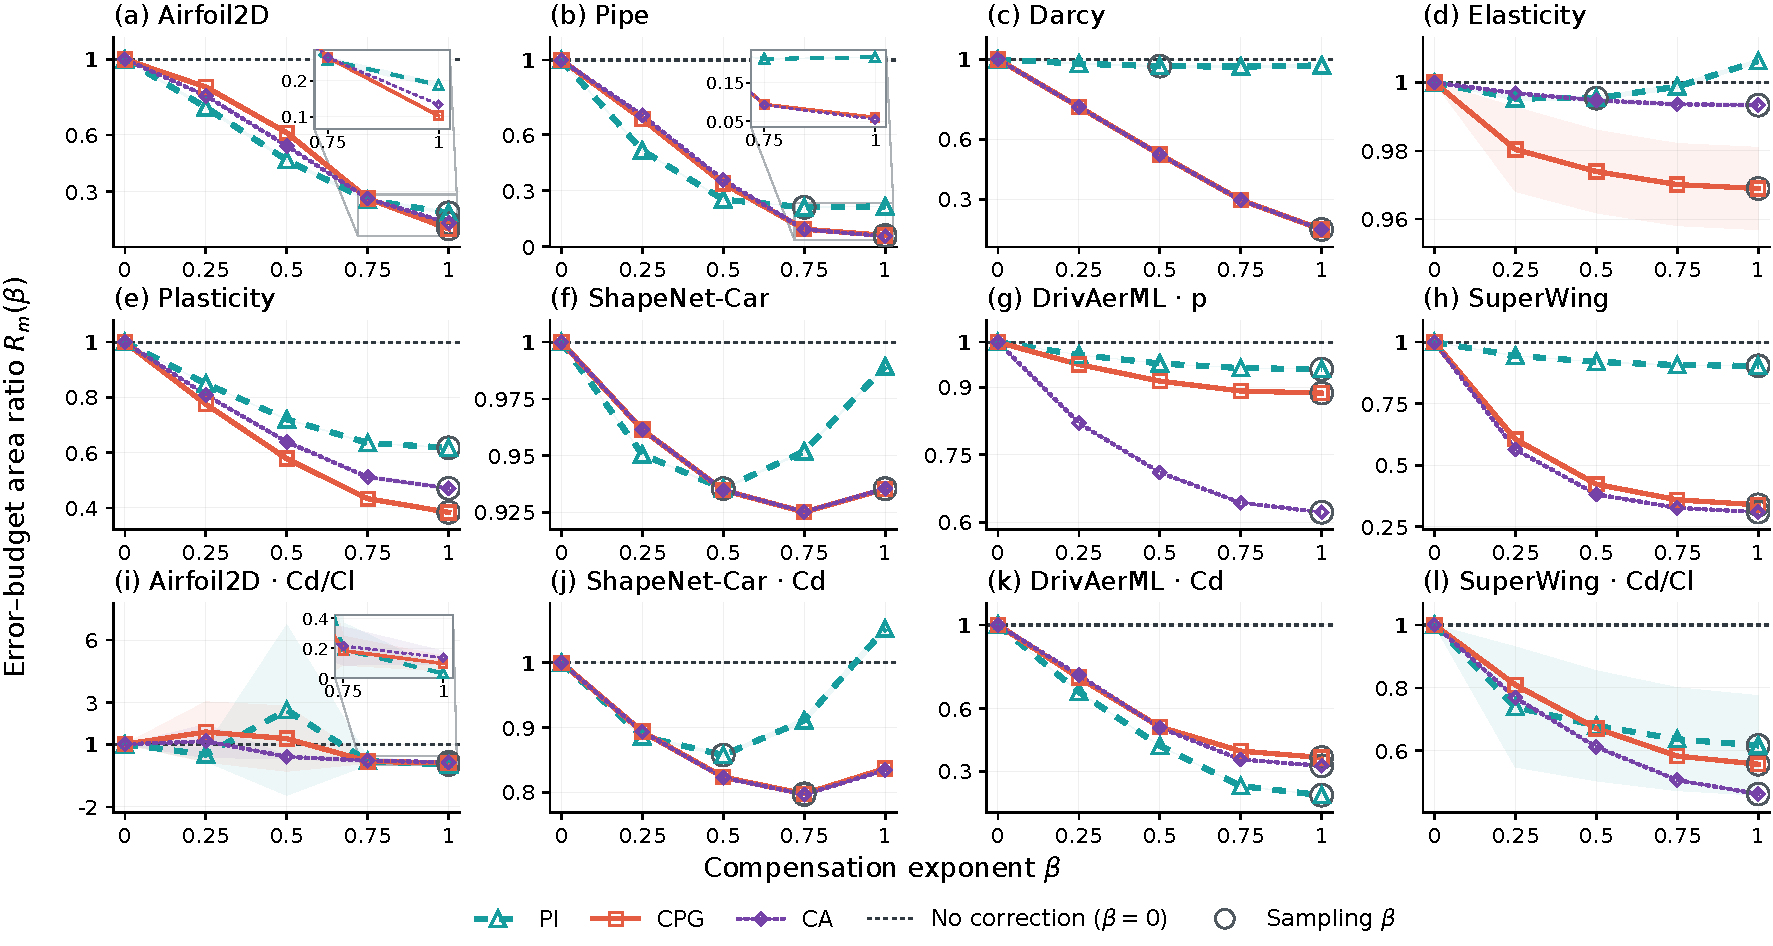
\includegraphics[width=\linewidth]{review_assets/baseline/d4021228aa183f7d5f7912124d17d3f69f8930b9/figures/appendix/beta_ablation.pdf}
%DIFDELCMD < %%%
\DIFdelendFL \DIFaddbeginFL 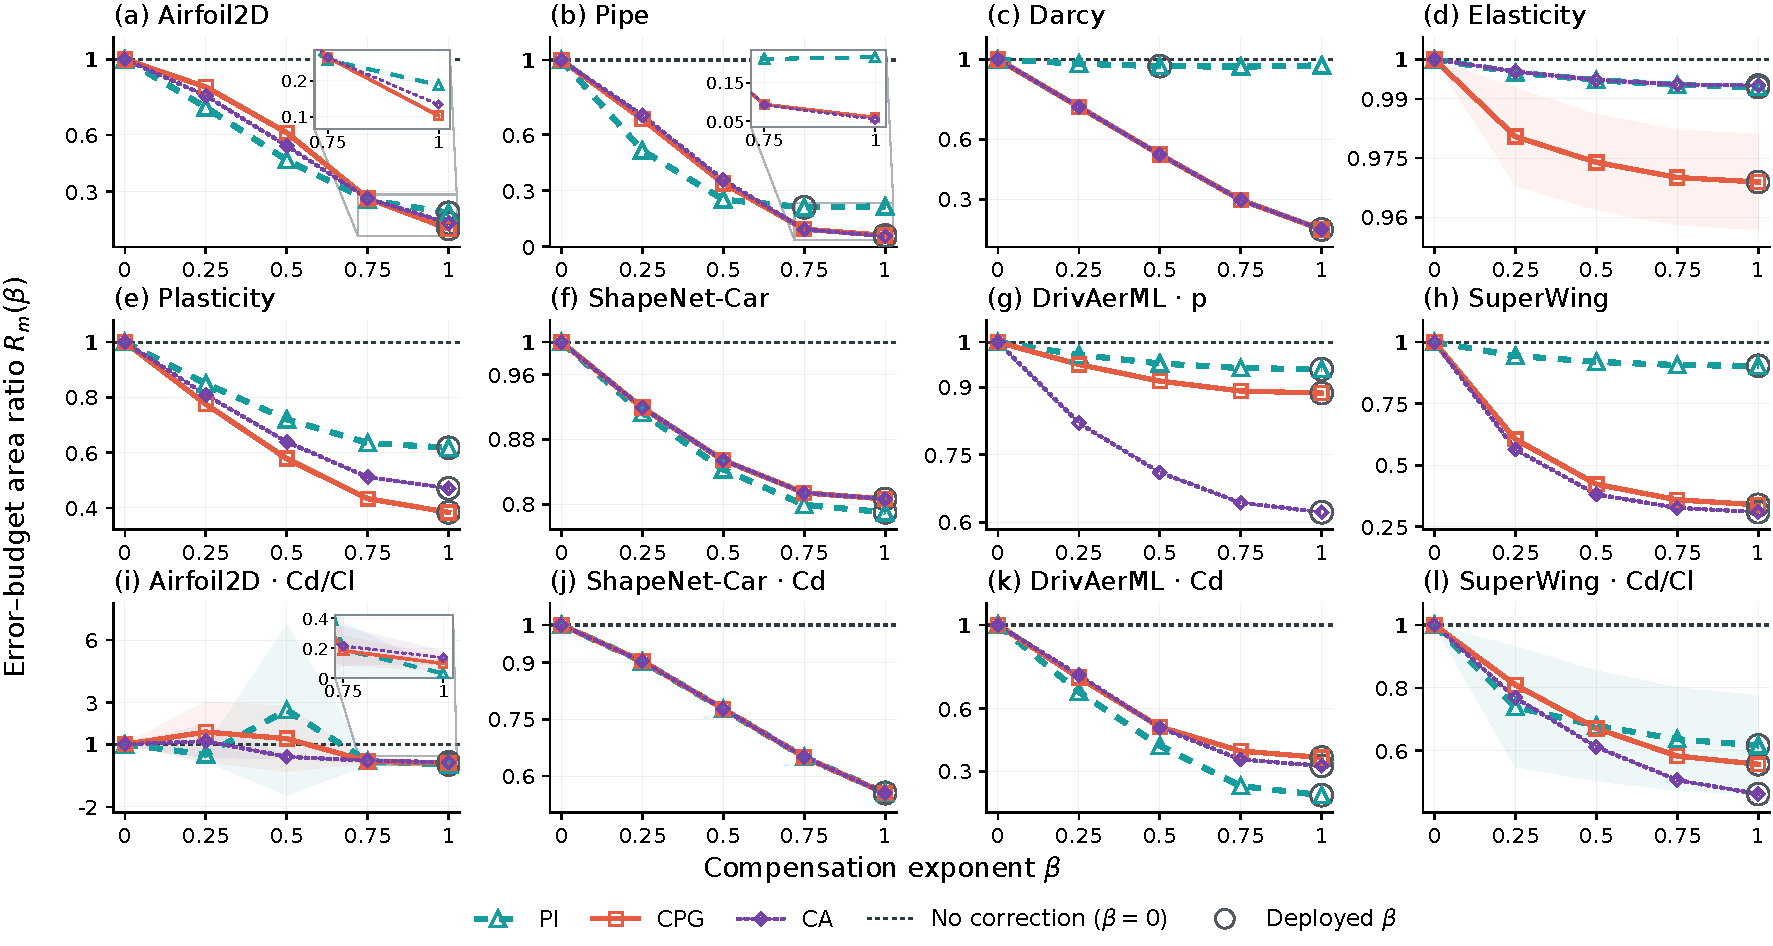
\includegraphics[width=\linewidth]{figures/appendix/beta_ablation.pdf}
\DIFaddendFL \caption{\textbf{Ablation of the measure-correction exponent.}
Checkpoints, sampled points, and reconstruction are fixed. The y-axis is
$R_m(\beta)$ from \eqref{eq:beta_relative_area}: each policy and seed is
normalized to its own $\beta=0$ error--budget area before averaging.
Areas cover $37.5\%$, $50\%$, and $75\%$ budgets. Bands show one sample
standard deviation across three \DIFaddbeginFL \DIFaddFL{sampling }\DIFaddendFL seeds. Gray rings (\DIFdelbeginFL \DIFdelFL{Sampling }\DIFdelendFL \DIFaddbeginFL \DIFaddFL{Deployed }\DIFaddendFL $\beta$) mark the
compensation exponent used by each policy in the main experiments.
The dashed line denotes no correction. Insets enlarge high-$\beta$
portions; the Airfoil ratio panel retains the full uncertainty envelope.
Table~\ref{tab:beta_ablation} uses Uniform-normalized rAUEC.}
\label{fig:beta_ablation}
\end{figure}


The results show a clear sensitivity to compensation mismatch.
Across most datasets and policies, the lowest or near-lowest error is
obtained when the inference-time correction is matched to the
policy-specific $\beta^\star$, while moving away from this setting
increases the error--budget area. This behavior is consistent with the
sampling-measure analysis: once the spatial samples are fixed, changing
$c_i^{\beta^\star}$ to $c_i^\beta$ changes the relative contribution of
the same point features to the physics tokens, introducing an aggregation
bias that propagates through the frozen operator.

The effect can be substantial. For CPG, removing the correction
($\beta=0$) increases the error--budget area by a factor of approximately
$9.7$ relative to full correction on Airfoil field prediction and by
approximately $16.4$ on Pipe. On Darcy, the CPG and CA rAUECs change from
$0.642$ and $0.640$ at their main-policy settings to $4.278$ and $4.265$
without compensation, despite using exactly the same sampled locations.
Similarly, the main correction reduces the SuperWing field
error--budget area by $66.1\%$ for CPG and $69.1\%$ for CA, and reduces
the DrivAerML drag area by $63.3\%$ and $67.3\%$, respectively.

\begin{table}[!htbp]
\centering
\small
\caption{Measure correction on fixed adaptive samples. Entries are mean rAUEC over three sampling seeds, with Uniform equal to one. Bold marks the lower value in each within-policy $\beta=0$/$\beta^{\star}$ pair. Parentheses give the percentage decrease in mean rAUEC from $\beta=0$, computed before rounding. \DIFdelbeginFL \DIFdelFL{The compensation exponents $\beta^{\star}$ are specified }\DIFdelendFL \DIFaddbeginFL \DIFaddFL{Elasticity PI and the ShapeNet-Car policies use $\beta^{\star}=1$. Gray rings }\DIFaddendFL in \DIFdelbeginFL \DIFdelFL{Appendix}\DIFdelendFL \DIFaddbeginFL \DIFaddFL{Figure}\DIFaddendFL ~\DIFdelbeginFL \DIFdelFL{\ref{app:density_policy_design}}\DIFdelendFL \DIFaddbeginFL \DIFaddFL{\ref{fig:beta_ablation} identify the deployed exponents}\DIFaddendFL .}
\label{tab:beta_ablation}
\setlength{\tabcolsep}{3pt}
\begin{tabular}{@{}llrrrrrr@{}}
\toprule
Dataset & Metric & \multicolumn{2}{c}{PI} & \multicolumn{2}{c}{CPG} & \multicolumn{2}{c}{CA} \\
\cmidrule(lr){3-4}\cmidrule(lr){5-6}\cmidrule(lr){7-8}
& & $\beta=0$ & $\beta^{\star}$ & $\beta=0$ & $\beta^{\star}$ & $\beta=0$ & $\beta^{\star}$ \\
\midrule
Airfoil & Field & 3.2852 & \textbf{0.6166}\,{\footnotesize (81.2\%)} & 5.6733 & \textbf{0.5831}\,{\footnotesize (89.7\%)} & 4.1829 & \textbf{0.5579}\,{\footnotesize (86.7\%)} \\
Pipe & Field & 4.1234 & \textbf{0.8711}\,{\footnotesize (78.9\%)} & 11.1004 & \textbf{0.6719}\,{\footnotesize (93.9\%)} & 12.7244 & \textbf{0.7051}\,{\footnotesize (94.5\%)} \\
Darcy & Field & 1.0315 & \textbf{0.9965}\,{\footnotesize (3.4\%)} & 4.2778 & \textbf{0.6419}\,{\footnotesize (85.0\%)} & 4.2654 & \textbf{0.6400}\,{\footnotesize (85.0\%)} \\
Elasticity & Field & 0.7314 & \shortstack[r]{\DIFdelFL{\textbf{0.7280}\,{\footnotesize (0.5\%)}}\\[1pt]\DIFaddFL{\textbf{0.7262}\,{\footnotesize (0.7\%)}}} & 0.4832 & \textbf{0.4681}\,{\footnotesize (3.1\%)} & 0.5506 & \textbf{0.5469}\,{\footnotesize (0.7\%)} \\
Plasticity & Field & 1.4393 & \textbf{0.8888}\,{\footnotesize (38.2\%)} & 2.3153 & \textbf{0.8890}\,{\footnotesize (61.6\%)} & 1.8908 & \textbf{0.8897}\,{\footnotesize (52.9\%)} \\
ShapeNet-Car & Field & 0.6301 & \shortstack[r]{\DIFdelFL{\textbf{0.5895}\,{\footnotesize (6.4\%)}}\\[1pt]\DIFaddFL{\textbf{0.4979}\,{\footnotesize (21.0\%)}}} & \shortstack[r]{\DIFdelFL{0.5962}\\[1pt]\DIFaddFL{0.6206}} & \shortstack[r]{\DIFdelFL{\textbf{0.5577}\,{\footnotesize (6.5\%)}}\\[1pt]\DIFaddFL{\textbf{0.5006}\,{\footnotesize (19.3\%)}}} & \shortstack[r]{\DIFdelFL{0.5962}\\[1pt]\DIFaddFL{0.6206}} & \shortstack[r]{\DIFdelFL{\textbf{0.5577}\,{\footnotesize (6.4\%)}}\\[1pt]\DIFaddFL{\textbf{0.5006}\,{\footnotesize (19.3\%)}}} \\
DrivAerML & Field & 0.9398 & \textbf{0.8834}\,{\footnotesize (6.0\%)} & 0.9298 & \textbf{0.8246}\,{\footnotesize (11.3\%)} & 1.3280 & \textbf{0.8263}\,{\footnotesize (37.8\%)} \\
SuperWing & Field & 0.8369 & \textbf{0.7564}\,{\footnotesize (9.6\%)} & 1.9796 & \textbf{0.6706}\,{\footnotesize (66.1\%)} & 2.3252 & \textbf{0.7193}\,{\footnotesize (69.1\%)} \\
Airfoil & Cd/Cl & 11.3964 & \textbf{0.2174}\,{\footnotesize (98.1\%)} & 2.1147 & \textbf{0.2379}\,{\footnotesize (88.7\%)} & 1.7583 & \textbf{0.2453}\,{\footnotesize (86.1\%)} \\
ShapeNet-Car & Cd & \shortstack[r]{\DIFdelFL{0.7649}\\[1pt]\DIFaddFL{1.1399}} & \shortstack[r]{\DIFdelFL{\textbf{0.6561}\,{\footnotesize (14.2\%)}}\\[1pt]\DIFaddFL{\textbf{0.6335}\,{\footnotesize (44.4\%)}}} & \shortstack[r]{\DIFdelFL{0.8113}\\[1pt]\DIFaddFL{1.1451}} & \shortstack[r]{\DIFdelFL{\textbf{0.6474}\,{\footnotesize (20.2\%)}}\\[1pt]\DIFaddFL{\textbf{0.6353}\,{\footnotesize (44.5\%)}}} & \shortstack[r]{\DIFdelFL{0.8130}\\[1pt]\DIFaddFL{1.1453}} & \shortstack[r]{\DIFdelFL{\textbf{0.6479}\,{\footnotesize (20.3\%)}}\\[1pt]\DIFaddFL{\textbf{0.6354}\,{\footnotesize (44.5\%)}}} \\
DrivAerML & Cd & 4.9553 & \textbf{0.9245}\,{\footnotesize (81.3\%)} & 2.5121 & \textbf{0.9209}\,{\footnotesize (63.3\%)} & 2.8282 & \textbf{0.9244}\,{\footnotesize (67.3\%)} \\
SuperWing & Cd/Cl & 1.4093 & \textbf{0.8246}\,{\footnotesize (41.5\%)} & 1.4403 & \textbf{0.8026}\,{\footnotesize (44.3\%)} & 1.7669 & \textbf{0.8167}\,{\footnotesize (53.8\%)} \\
\bottomrule
\end{tabular}
\end{table}


\DIFdelbegin \DIFdel{The non-unit optimal exponents provide an especially informative control.
For example, on }\DIFdelend \DIFaddbegin \DIFadd{Elasticity PI and all }\DIFaddend ShapeNet-Car \DIFdelbegin \DIFdel{drag prediction, CPG and CA attain their
lowest areas around the policy value $\beta^\star=0.75$, rather than at
$\beta=1$, while PI favors the smaller correction used by its policy. Thus, }\DIFdelend \DIFaddbegin \DIFadd{policies use $\beta^\star=1$.
Relative to $\beta=0$ on }\DIFaddend the \DIFdelbegin \DIFdel{observed improvement is not simply a consequence of applying
stronger reweighting. Instead, inference is most accurate when the compensation strength is consistent with that used to construct the
corresponding adaptive }\DIFdelend \DIFaddbegin \DIFadd{same sampled points, full correction reduces
mean rAUEC by $0.7\%$ for Elasticity PI. On ShapeNet-Car, it reduces field
rAUEC by $19.3$--$21.0\%$ and drag rAUEC by $44.4$--$44.5\%$ across the
three policies. These comparisons quantify the benefit of reference-measure
compensation for each fixed adaptive sampling }\DIFaddend policy.

Overall, this controlled experiment provides direct empirical evidence
for the sampling-measure bias analyzed in
Section~\ref{sec:density_consistent_transolver}. Adaptive sampling
determines \emph{where} the frozen operator is evaluated, while the
measure correction determines \emph{how} those sampled features are
aggregated. Holding the former fixed and perturbing only the latter
shows that a mismatch in compensation can substantially degrade
prediction accuracy, whereas the policy-matched correction restores the
intended inference behavior.
\DIFaddbegin 

\DIFaddend \clearpage

\subsection{More Results}
\label{app:budget_curves}

Figure~\ref{fig:appendix_budget_curves} compares Uniform and the three
AdaSolver policies at $37.5\%$, $50\%$, and $75\%$ point budgets with
full-mesh-trained Transolver references, including their $100\%$ endpoints.
Errors are divided by the full-mesh error of the backbone shared by Uniform
and AdaSolver; the horizontal line at one marks this reference. Shaded bands
show one sample standard deviation across three sampling seeds.

References use the original Transolver checkpoints for Pipe and Elasticity,
and task-specific checkpoints trained on full meshes for the remaining
tasks. Point-cloud models reuse Uniform's
samples and reconstruction; Pipe uses Cartesian subgrids at the plotted
retained fractions. Darcy's full-mesh-trained backbone makes its two curves
coincide. DrivAerML changes the pressure checkpoint while retaining Uniform's
wall-shear-stress predictions. The Airfoil reference is trained on pressure
using all 11,271 points per training step, with the same architecture,
1,000 epochs, and global batch of eight as the variable-point backbone.
Both Airfoil panels use the same 110 cases and the shared pressure backbone's
full-mesh error for normalization. Airfoil $C_D/C_L$ uses absolute ratio error.
Its axis is linear through five and logarithmic above five, with the
transition marked. Elasticity uses a logarithmic axis.

On Plasticity, CPG at
$37.5\%$ achieves $5.02\%$ relative $L_2$ error, compared with $6.40\%$ for
Transolver at $100\%$: $62.5\%$ fewer points and $21.6\%$ lower error.
On DrivAerML, the corresponding $C_D$ errors are $0.948\%$ and $1.05\%$.
On Airfoil, CPG at $37.5\%$ gives $0.0186$ absolute $C_D/C_L$ error,
compared with $0.0281$ for the full-mesh-trained reference at $100\%$.
The benefit depends on the task and output quantity: in Darcy, CPG and CA
approach full-mesh field accuracy at small budgets, while PI stays close to
Uniform.

\begin{figure}[!ht]
    \centering
    \DIFdelbeginFL %DIFDELCMD < 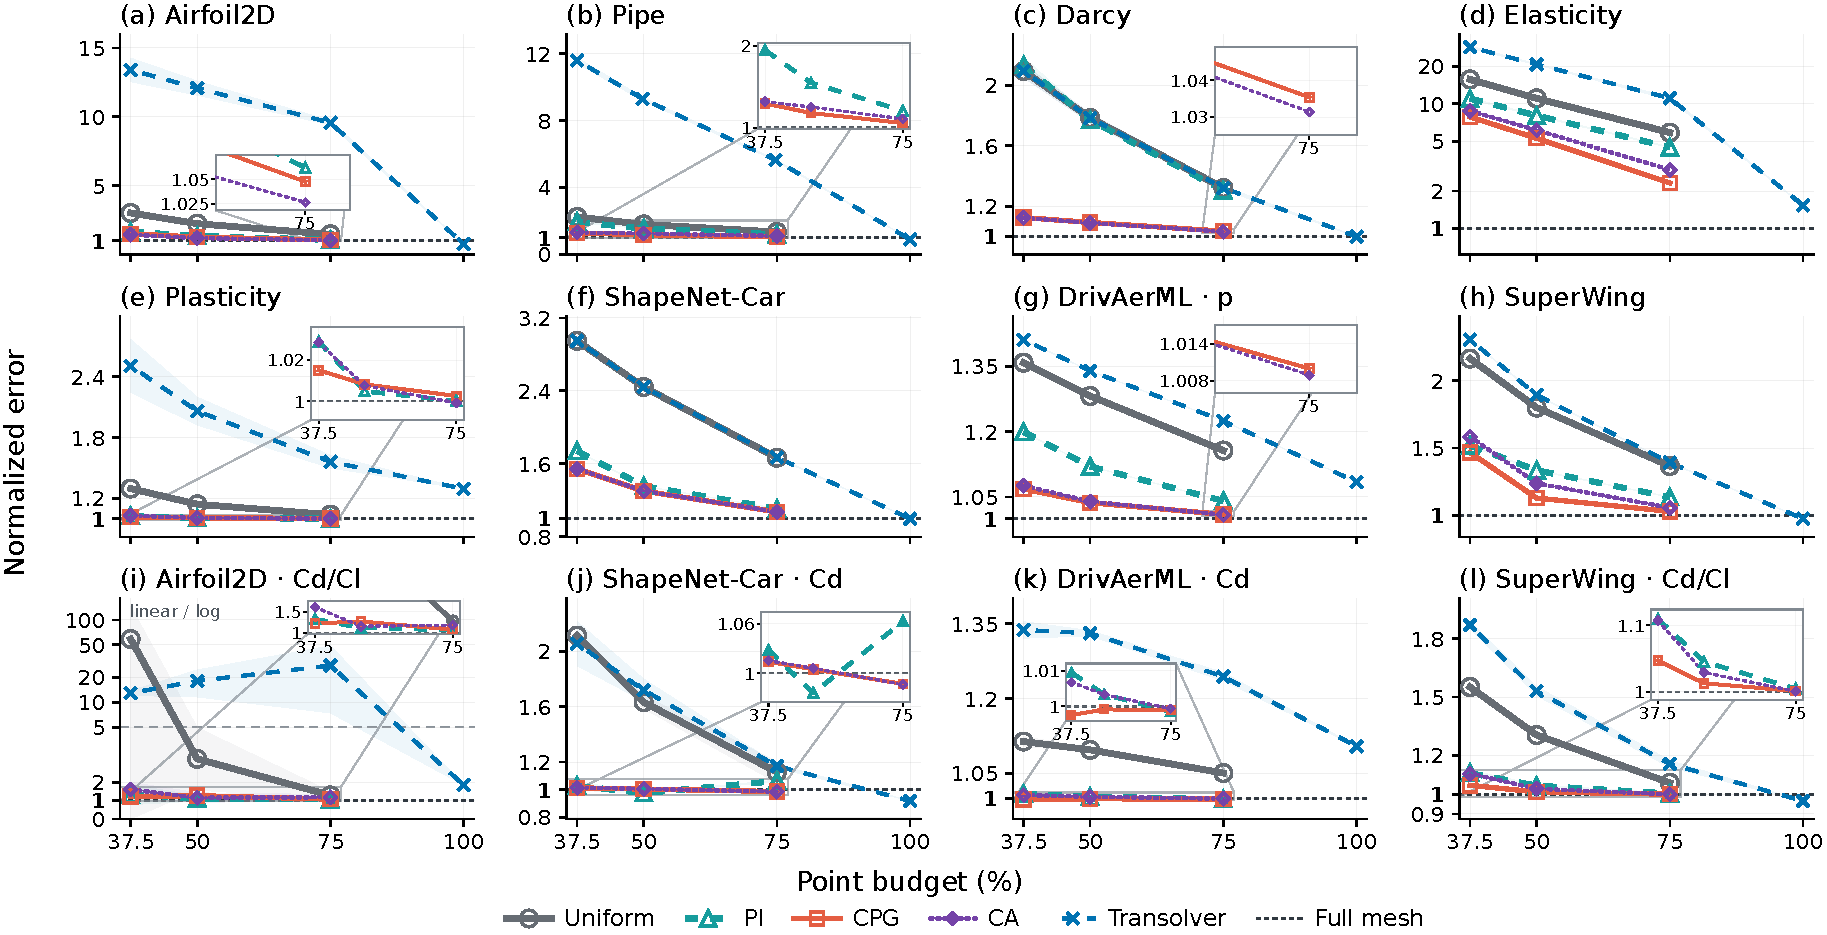
\includegraphics[width=\linewidth]{review_assets/baseline/d4021228aa183f7d5f7912124d17d3f69f8930b9/figures/appendix/budget_error_curves.pdf}
%DIFDELCMD <     %%%
\DIFdelendFL \DIFaddbeginFL 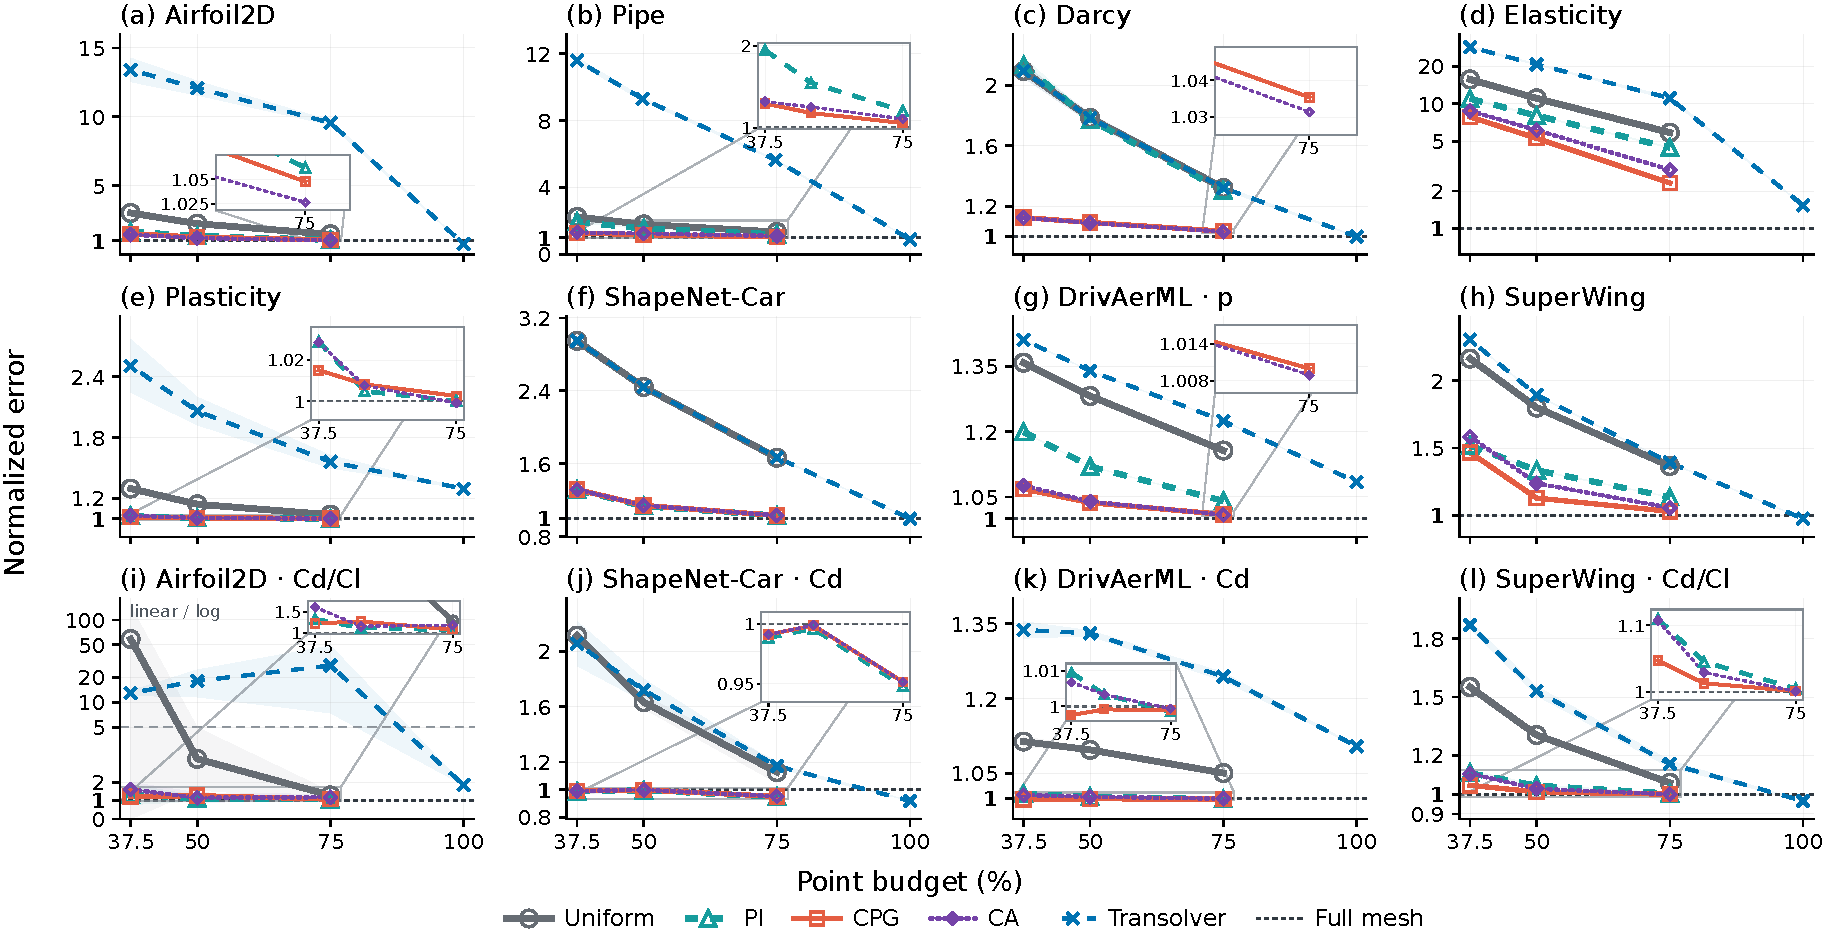
\includegraphics[width=\linewidth]{figures/appendix/budget_error_curves.pdf}
    \DIFaddendFL \caption{\textbf{Accuracy across point budgets.}
Panels (a)--(h) show field metrics and (i)--(l) show aerodynamic quantities.
Transolver is the full-mesh-trained reference; the horizontal line marks
full-mesh accuracy of AdaSolver's backbone. \DIFaddbeginFL \DIFaddFL{Elasticity PI and the three
ShapeNet-Car policies use $\beta=1$. }\DIFaddendFL Airfoil uses 110 cases with reference
$C_L>0.02$ and a pressure-trained Transolver reference. Its $C_D/C_L$ axis
is linear through five, then logarithmic. Insets enlarge mean curves.}
    \label{fig:appendix_budget_curves}
\end{figure}

\clearpage
\subsection{Density Visualization}
\label{app:density_visualization}

Figure~\ref{fig:appendix_density_visualization} compares point allocation
for the eight showcase cases at a $37.5\%$ budget. Within each spatial bin
$B$, we display the retained fraction
$n_{\mathrm{selected}}(B)/n_{\mathrm{reference}}(B)$ on a common scale.
Uniform gives approximately constant retention, while the adaptive policies
redistribute points across the domain.

\begin{figure}[!ht]
    \centering
    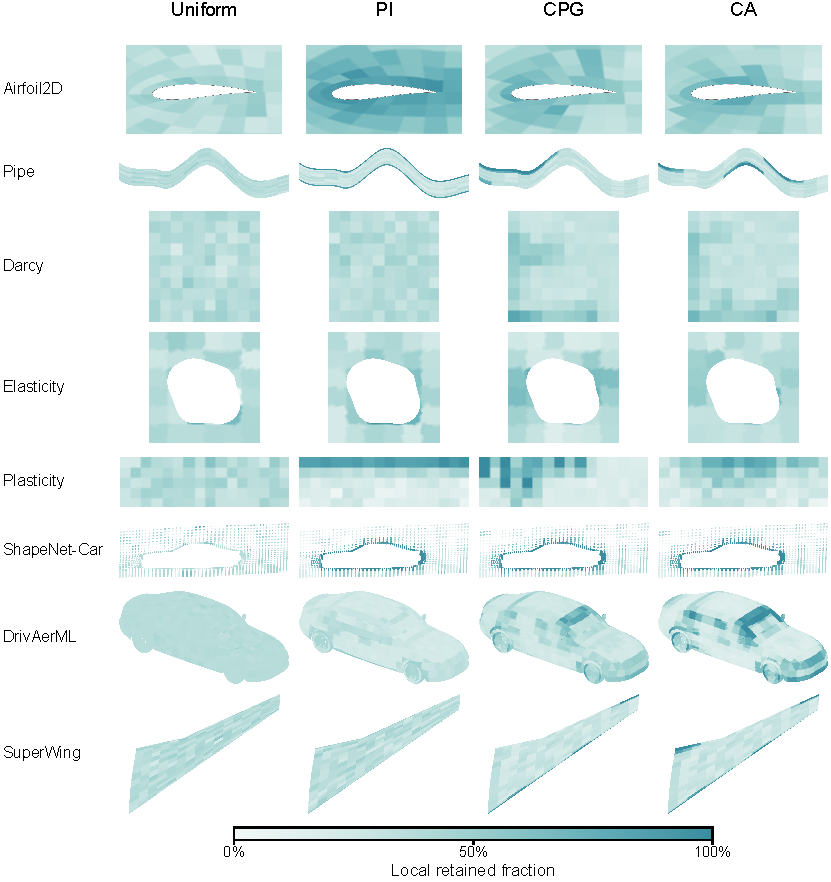
\includegraphics[width=\linewidth,height=.74\textheight,keepaspectratio]{figures/appendix/density_visualization.pdf}
    \caption{\textbf{Local sampling retention.} Rows show the same eight
    cases used in Appendix~\ref{app:field_visualizations}, with sampling
    seed zero. Darker colors indicate a larger fraction of reference points
    retained within each bin. All methods share the same color scale.}
    \label{fig:appendix_density_visualization}
\end{figure}


\clearpage
\subsection{COMPUTATIONAL COST}
\label{app:computational_cost}

Adaptive inference reduces operator evaluation cost by processing fewer
spatial points, but introduces additional overhead for acquiring the
refinement signal. Table~\ref{tab:inference_time_sampled}
quantifies this trade-off across all eight benchmarks at the three
evaluation budgets. All methods use the same frozen backbone. Uniform
provides a reference at matched point counts, while full mesh measures the
cost of evaluating all reference points. The reported latency includes
online refinement and prediction at the selected points, with reusable
preprocessing performed in advance. Reconstruction onto the full mesh is
excluded.

\begin{table}[!ht]
\centering
\begingroup
\footnotesize
\setlength{\tabcolsep}{3.0pt}
\renewcommand{\arraystretch}{1.08}
\begin{tabular}{llrrrrr}
\toprule
Task & Budget & Full mesh & Uniform & PI & CPG & CA \\
\midrule
Airfoil2D & 37.5\% & $5.280\!\pm\!0.009$ & $2.438\!\pm\!0.018$ & $2.539\!\pm\!0.016$ & $4.435\!\pm\!0.039$ & $3.110\!\pm\!0.031$ \\
 & 50\% &  & $3.037\!\pm\!0.005$ & $3.176\!\pm\!0.006$ & $5.050\!\pm\!0.012$ & $3.775\!\pm\!0.012$ \\
 & 75\% &  & $4.049\!\pm\!0.009$ & $4.218\!\pm\!0.013$ & $6.104\!\pm\!0.018$ & $4.847\!\pm\!0.016$ \\
\addlinespace[2pt]
Pipe & 37.5\% & $7.407\!\pm\!0.004$ & $3.238\!\pm\!0.002$ & $3.382\!\pm\!0.004$ & $5.067\!\pm\!0.005$ & $4.095\!\pm\!0.005$ \\
 & 50\% &  & $4.038\!\pm\!0.005$ & $4.199\!\pm\!0.005$ & $5.891\!\pm\!0.007$ & $4.923\!\pm\!0.007$ \\
 & 75\% &  & $5.780\!\pm\!0.021$ & $6.025\!\pm\!0.016$ & $7.721\!\pm\!0.020$ & $6.774\!\pm\!0.028$ \\
\addlinespace[2pt]
Darcy & 37.5\% & $3.525\!\pm\!0.001$ & $1.929\!\pm\!0.002$ & $1.994\!\pm\!0.003$ & $3.469\!\pm\!0.007$ & $2.675\!\pm\!0.004$ \\
 & 50\% &  & $2.212\!\pm\!0.001$ & $2.301\!\pm\!0.003$ & $3.785\!\pm\!0.017$ & $3.002\!\pm\!0.015$ \\
 & 75\% &  & $2.907\!\pm\!0.005$ & $3.030\!\pm\!0.004$ & $4.536\!\pm\!0.014$ & $3.738\!\pm\!0.006$ \\
\addlinespace[2pt]
Elasticity$\dagger$ & 37.5\% & $1.264\!\pm\!0.013$ & $0.987\!\pm\!0.007$ & $1.009\!\pm\!0.006$ & $2.086\!\pm\!0.013$ & $1.524\!\pm\!0.024$ \\
 & 50\% &  & $1.027\!\pm\!0.004$ & $1.047\!\pm\!0.003$ & $2.209\!\pm\!0.003$ & $1.598\!\pm\!0.017$ \\
 & 75\% &  & $1.166\!\pm\!0.003$ & $1.184\!\pm\!0.004$ & $2.401\!\pm\!0.038$ & $1.756\!\pm\!0.012$ \\
\addlinespace[2pt]
Plasticity & 37.5\% & $2.049\!\pm\!0.006$ & $1.259\!\pm\!0.002$ & $1.289\!\pm\!0.003$ & $2.516\!\pm\!0.005$ & $1.657\!\pm\!0.003$ \\
 & 50\% &  & $1.430\!\pm\!0.002$ & $1.470\!\pm\!0.002$ & $2.716\!\pm\!0.007$ & $1.833\!\pm\!0.004$ \\
 & 75\% &  & $1.708\!\pm\!0.062$ & $1.772\!\pm\!0.071$ & $3.049\!\pm\!0.065$ & $2.152\!\pm\!0.078$ \\
\addlinespace[2pt]
ShapeNet-Car & 37.5\% & $16.359\!\pm\!0.011$ & $6.856\!\pm\!0.004$ & $6.976\!\pm\!0.005$ & $10.609\!\pm\!0.026$ & $8.401\!\pm\!0.027$ \\
 & 50\% &  & $8.644\!\pm\!0.008$ & $8.773\!\pm\!0.006$ & $12.404\!\pm\!0.025$ & $10.259\!\pm\!0.027$ \\
 & 75\% &  & $12.388\!\pm\!0.004$ & $12.618\!\pm\!0.006$ & $16.258\!\pm\!0.029$ & $14.148\!\pm\!0.029$ \\
\addlinespace[2pt]
DrivAerML & 37.5\% & $4601.5\!\pm\!140.1$ & $1726.7\!\pm\!46.4$ & $1758.6\!\pm\!47.6$ & $2228.2\!\pm\!61.2$ & $1765.0\!\pm\!46.6$ \\
 & 50\% &  & $2306.9\!\pm\!62.1$ & $2347.1\!\pm\!62.2$ & $2825.2\!\pm\!74.3$ & $2345.7\!\pm\!59.6$ \\
 & 75\% &  & $3460.8\!\pm\!97.0$ & $3520.6\!\pm\!97.2$ & $4005.8\!\pm\!109.6$ & $3505.5\!\pm\!94.4$ \\
\addlinespace[2pt]
SuperWing & 37.5\% & $13.602\!\pm\!0.010$ & $5.671\!\pm\!0.002$ & $5.909\!\pm\!0.003$ & $8.610\!\pm\!0.006$ & $6.659\!\pm\!0.007$ \\
 & 50\% &  & $7.401\!\pm\!0.005$ & $7.744\!\pm\!0.005$ & $10.447\!\pm\!0.007$ & $8.487\!\pm\!0.006$ \\
 & 75\% &  & $10.483\!\pm\!0.010$ & $10.987\!\pm\!0.008$ & $13.690\!\pm\!0.010$ & $11.763\!\pm\!0.010$ \\
\bottomrule
\end{tabular}
\endgroup
\caption{\textbf{Inference latency at different point budgets (ms).}
Values are means $\pm$ standard deviations across test cases and repeated samplings.
The full-mesh column uses all reference points and three cases, and is shown once per task.
$\dagger$ The Elasticity timing configuration uses a $25\%$ coarse set and a two-block head.
Timings cover prediction at the selected points and online refinement, excluding full-field reconstruction.}
\label{tab:inference_time_sampled}
\end{table}


\paragraph{Refinement overhead.}
PI remains close to Uniform, adding $1.5$--$4.8\%$ latency across the
24 task--budget pairs. Its geometry-based density can be reused across
predictions. CPG incurs a larger overhead because it evaluates a complete
coarse prediction before selecting additional points. CA obtains its
refinement signal from early features and reuses cached pointwise
quantities during the final evaluation. It reduces latency by
$12.3$--$34.1\%$ relative to CPG, with a reduction in every measured
setting. Thus, the learned refinement signal substantially reduces the
runtime overhead of input-adaptive sampling compared with
coarse-prediction-based refinement.

\paragraph{Realized speedup.}
At a $37.5\%$ point budget, CA is faster than full-mesh inference on seven
of the eight benchmarks. The speedups, computed as
$T_{\mathrm{full}}/T_{\mathrm{CA}}$, reach $1.95\times$ on ShapeNet-Car,
$2.61\times$ on DrivAerML, and $2.04\times$ on SuperWing.
These gains are more pronounced when
point-dependent operator evaluation constitutes a large fraction of the
total inference cost. On Elasticity, CA takes $1.52$~ms versus $1.26$~ms
for full mesh: refinement overhead exceeds the savings in point-dependent
computation.
Point reduction does not imply a proportional reduction in latency.
Consequently, the realized speedup is governed by the balance between the
operator computation eliminated by point reduction and the additional
cost of acquiring the refinement signal.


\clearpage
\subsection{More Showcases}
\label{app:field_visualizations}

The following pages connect the aggregate error profiles to spatial sampling
and reconstruction. Each page shows one held-out geometry at a $37.5\%$ point
budget with sampling seed zero. These examples were selected for visible
differences between sampling policies. Their annotations report errors for
the displayed case. Figure~\ref{fig:appendix_budget_curves} summarizes
the test populations.

The first two rows show sampling locations and the policy's refinement
feature. Features are rescaled from each policy's minimum to its 99th
percentile for display, with larger values clipped at the upper end of the
colour scale. Uniform has no refinement feature. Each physical quantity then
has a ground-truth view and matched prediction and error rows. Field and
error ranges are shared across methods within that quantity. Colour-bar
arrows indicate values outside the displayed range. Component errors are
signed prediction-minus-ground-truth residuals. Magnitude rows show
nonnegative vector error norms, and Plasticity uses the temporal aggregation
specified below.

\subsubsection{Airfoil}
\label{app:vis_airfoil}

The pressure jump in this example makes errors in its location visible as
a narrow residual band. All three adaptive policies reduce the field error
relative to Uniform. CA gives the lowest error for this geometry ($1.30\%$),
with PI and CPG attaining $1.33\%$ and $1.35\%$, respectively.

\begin{figure}[!ht]
    \centering
    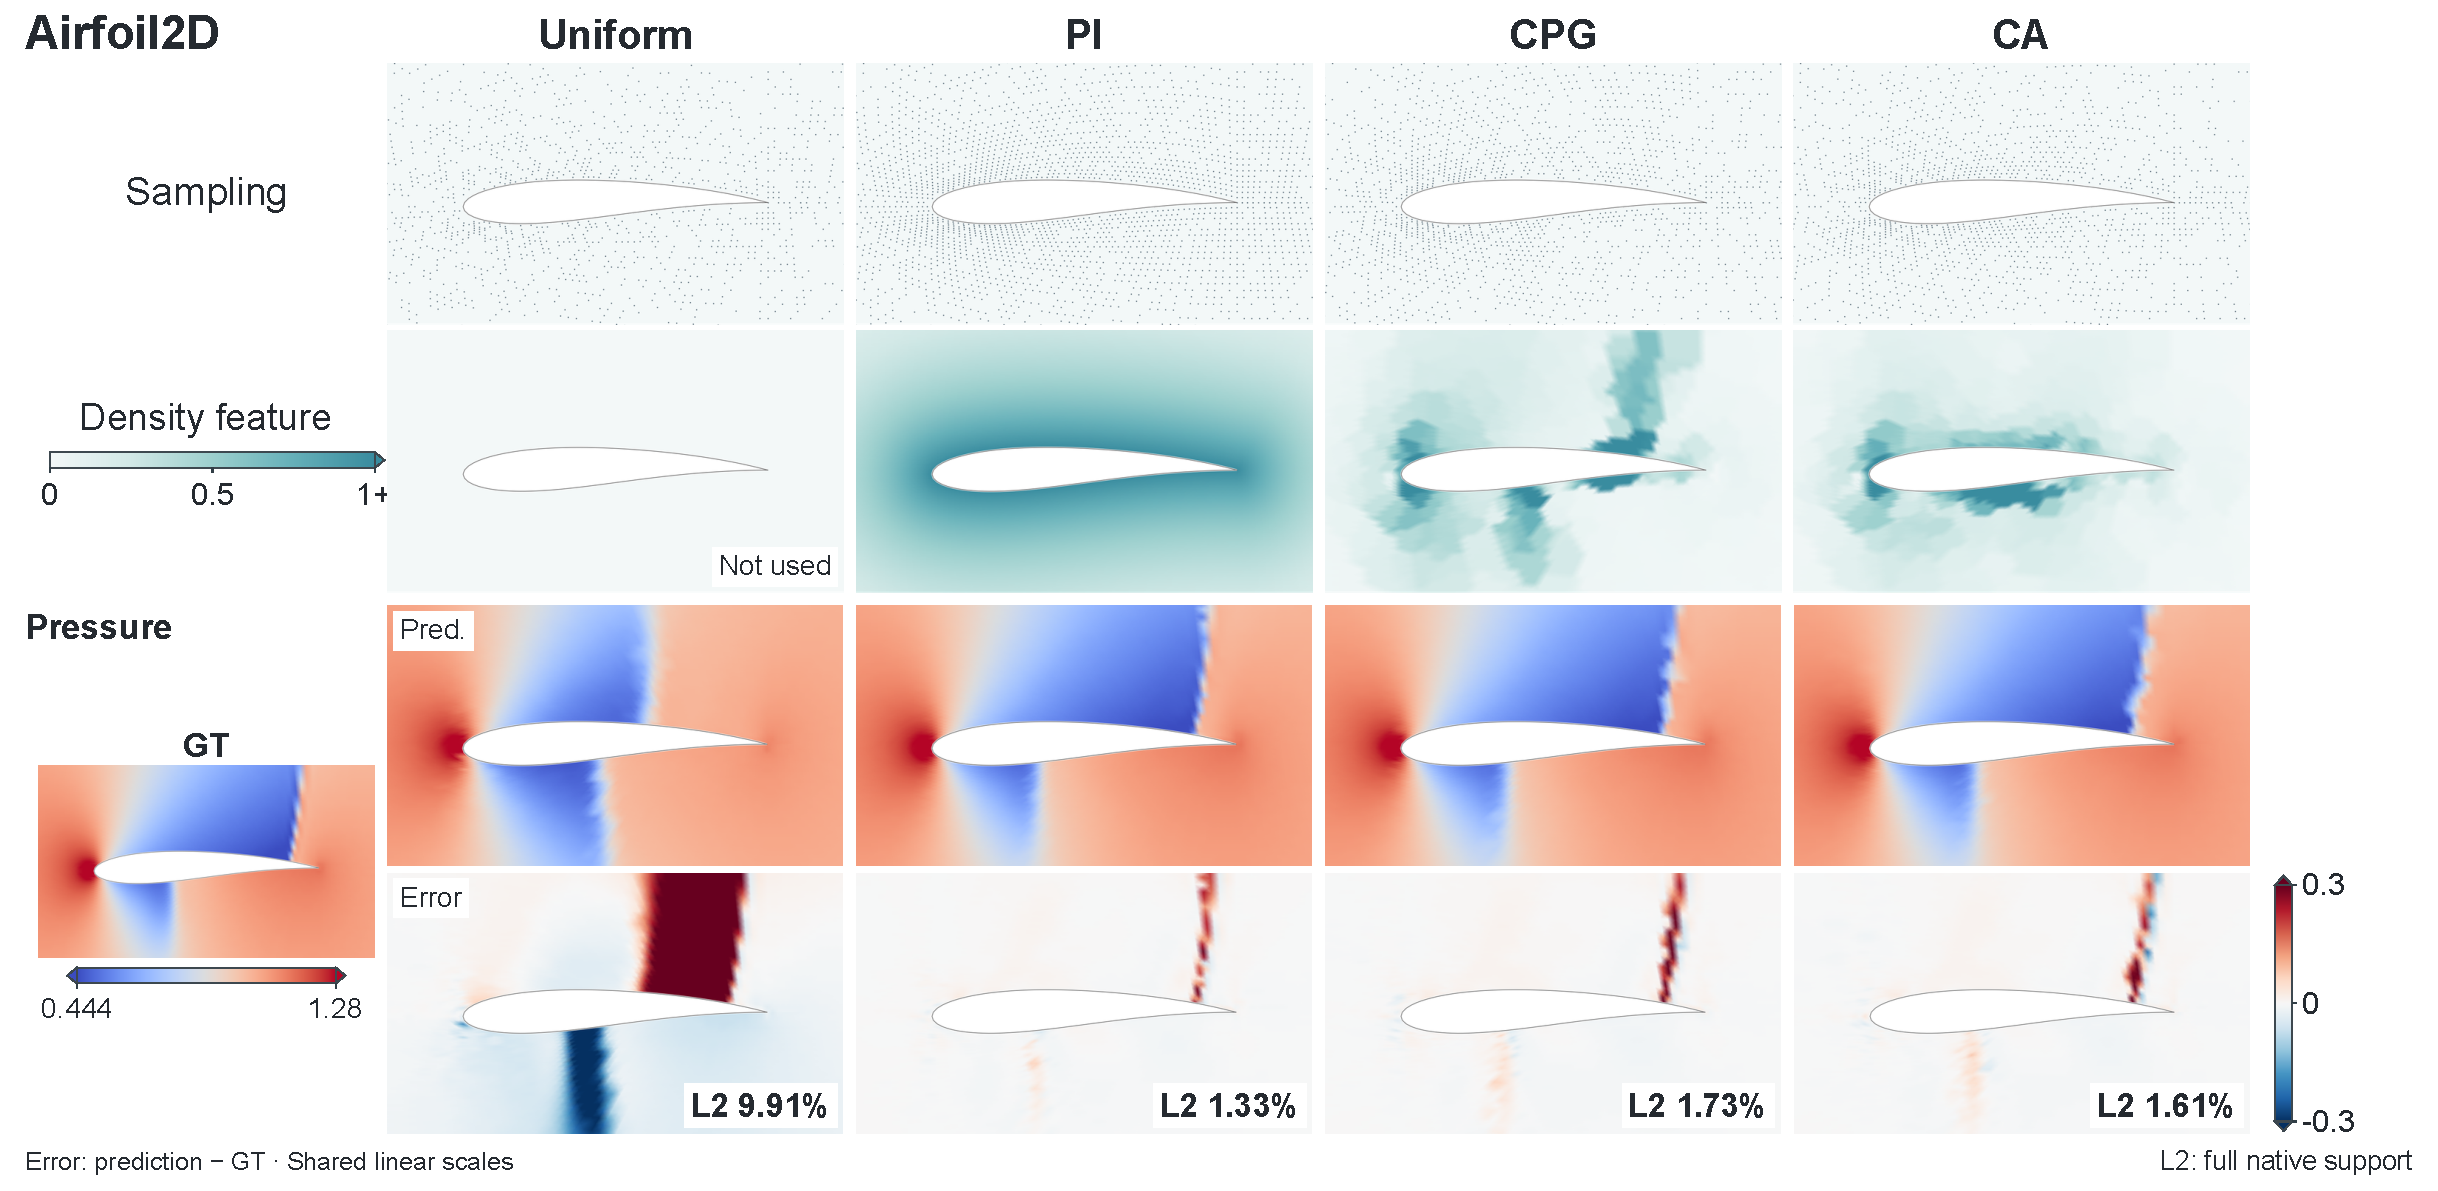
\includegraphics[width=\linewidth,height=.69\textheight,keepaspectratio]{figures/appendix/airfoil2d_fields.pdf}
    \caption{\textbf{Airfoil.} Sampling and pressure prediction.}
    \label{fig:appendix_airfoil}
\end{figure}

\clearpage
\subsubsection{Pipe}
\label{app:vis_pipe}

The predicted horizontal-velocity fields have similar overall structure,
while the shared residual scale exposes differences along the curved pipe.
CPG and CA reduce the error to $0.24\%$ and $0.30\%$, respectively,
compared with $1.31\%$ under Uniform sampling.

\begin{figure}[!ht]
    \centering
    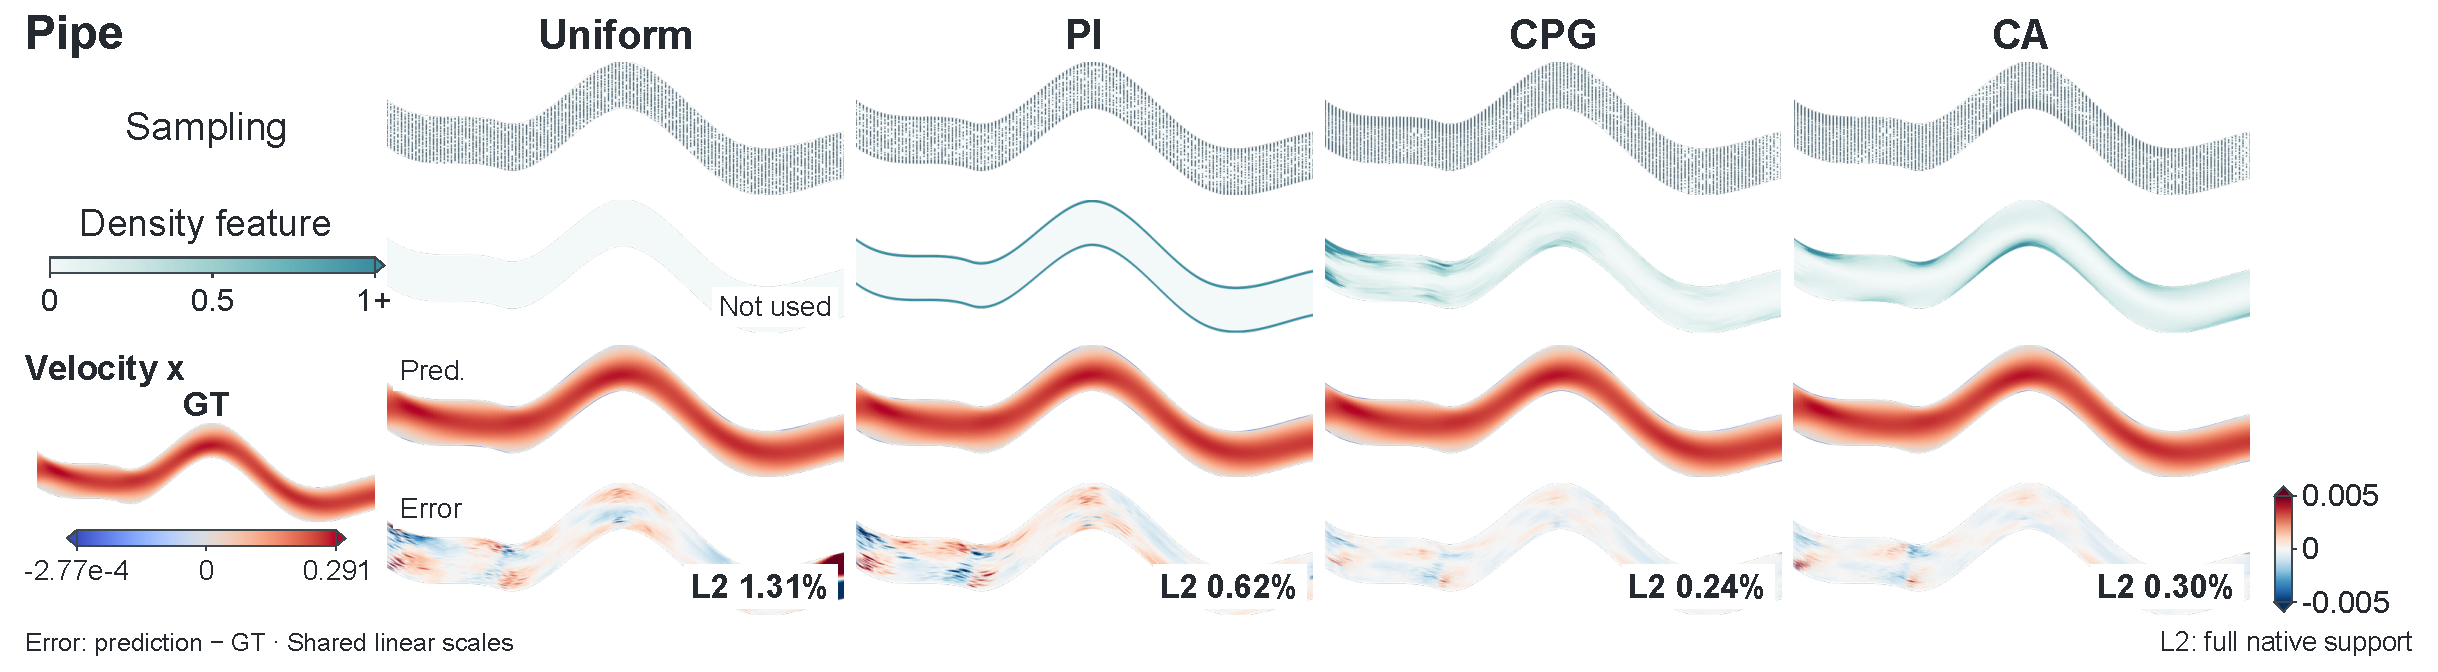
\includegraphics[width=\linewidth,height=.69\textheight,keepaspectratio]{figures/appendix/pipe_fields.pdf}
    \caption{\textbf{Pipe.} Sampling and horizontal velocity prediction.}
    \label{fig:appendix_pipe}
\end{figure}

\clearpage
\subsubsection{Darcy}
\label{app:vis_darcy}

The refinement policies assign different importance to regions of the
heterogeneous medium. The CPG and CA allocations produce similar solution
fields and smaller residuals than Uniform in this example, consistent with
their aggregate advantage on Darcy in Figure~\ref{fig:appendix_budget_curves}.

\begin{figure}[!ht]
    \centering
    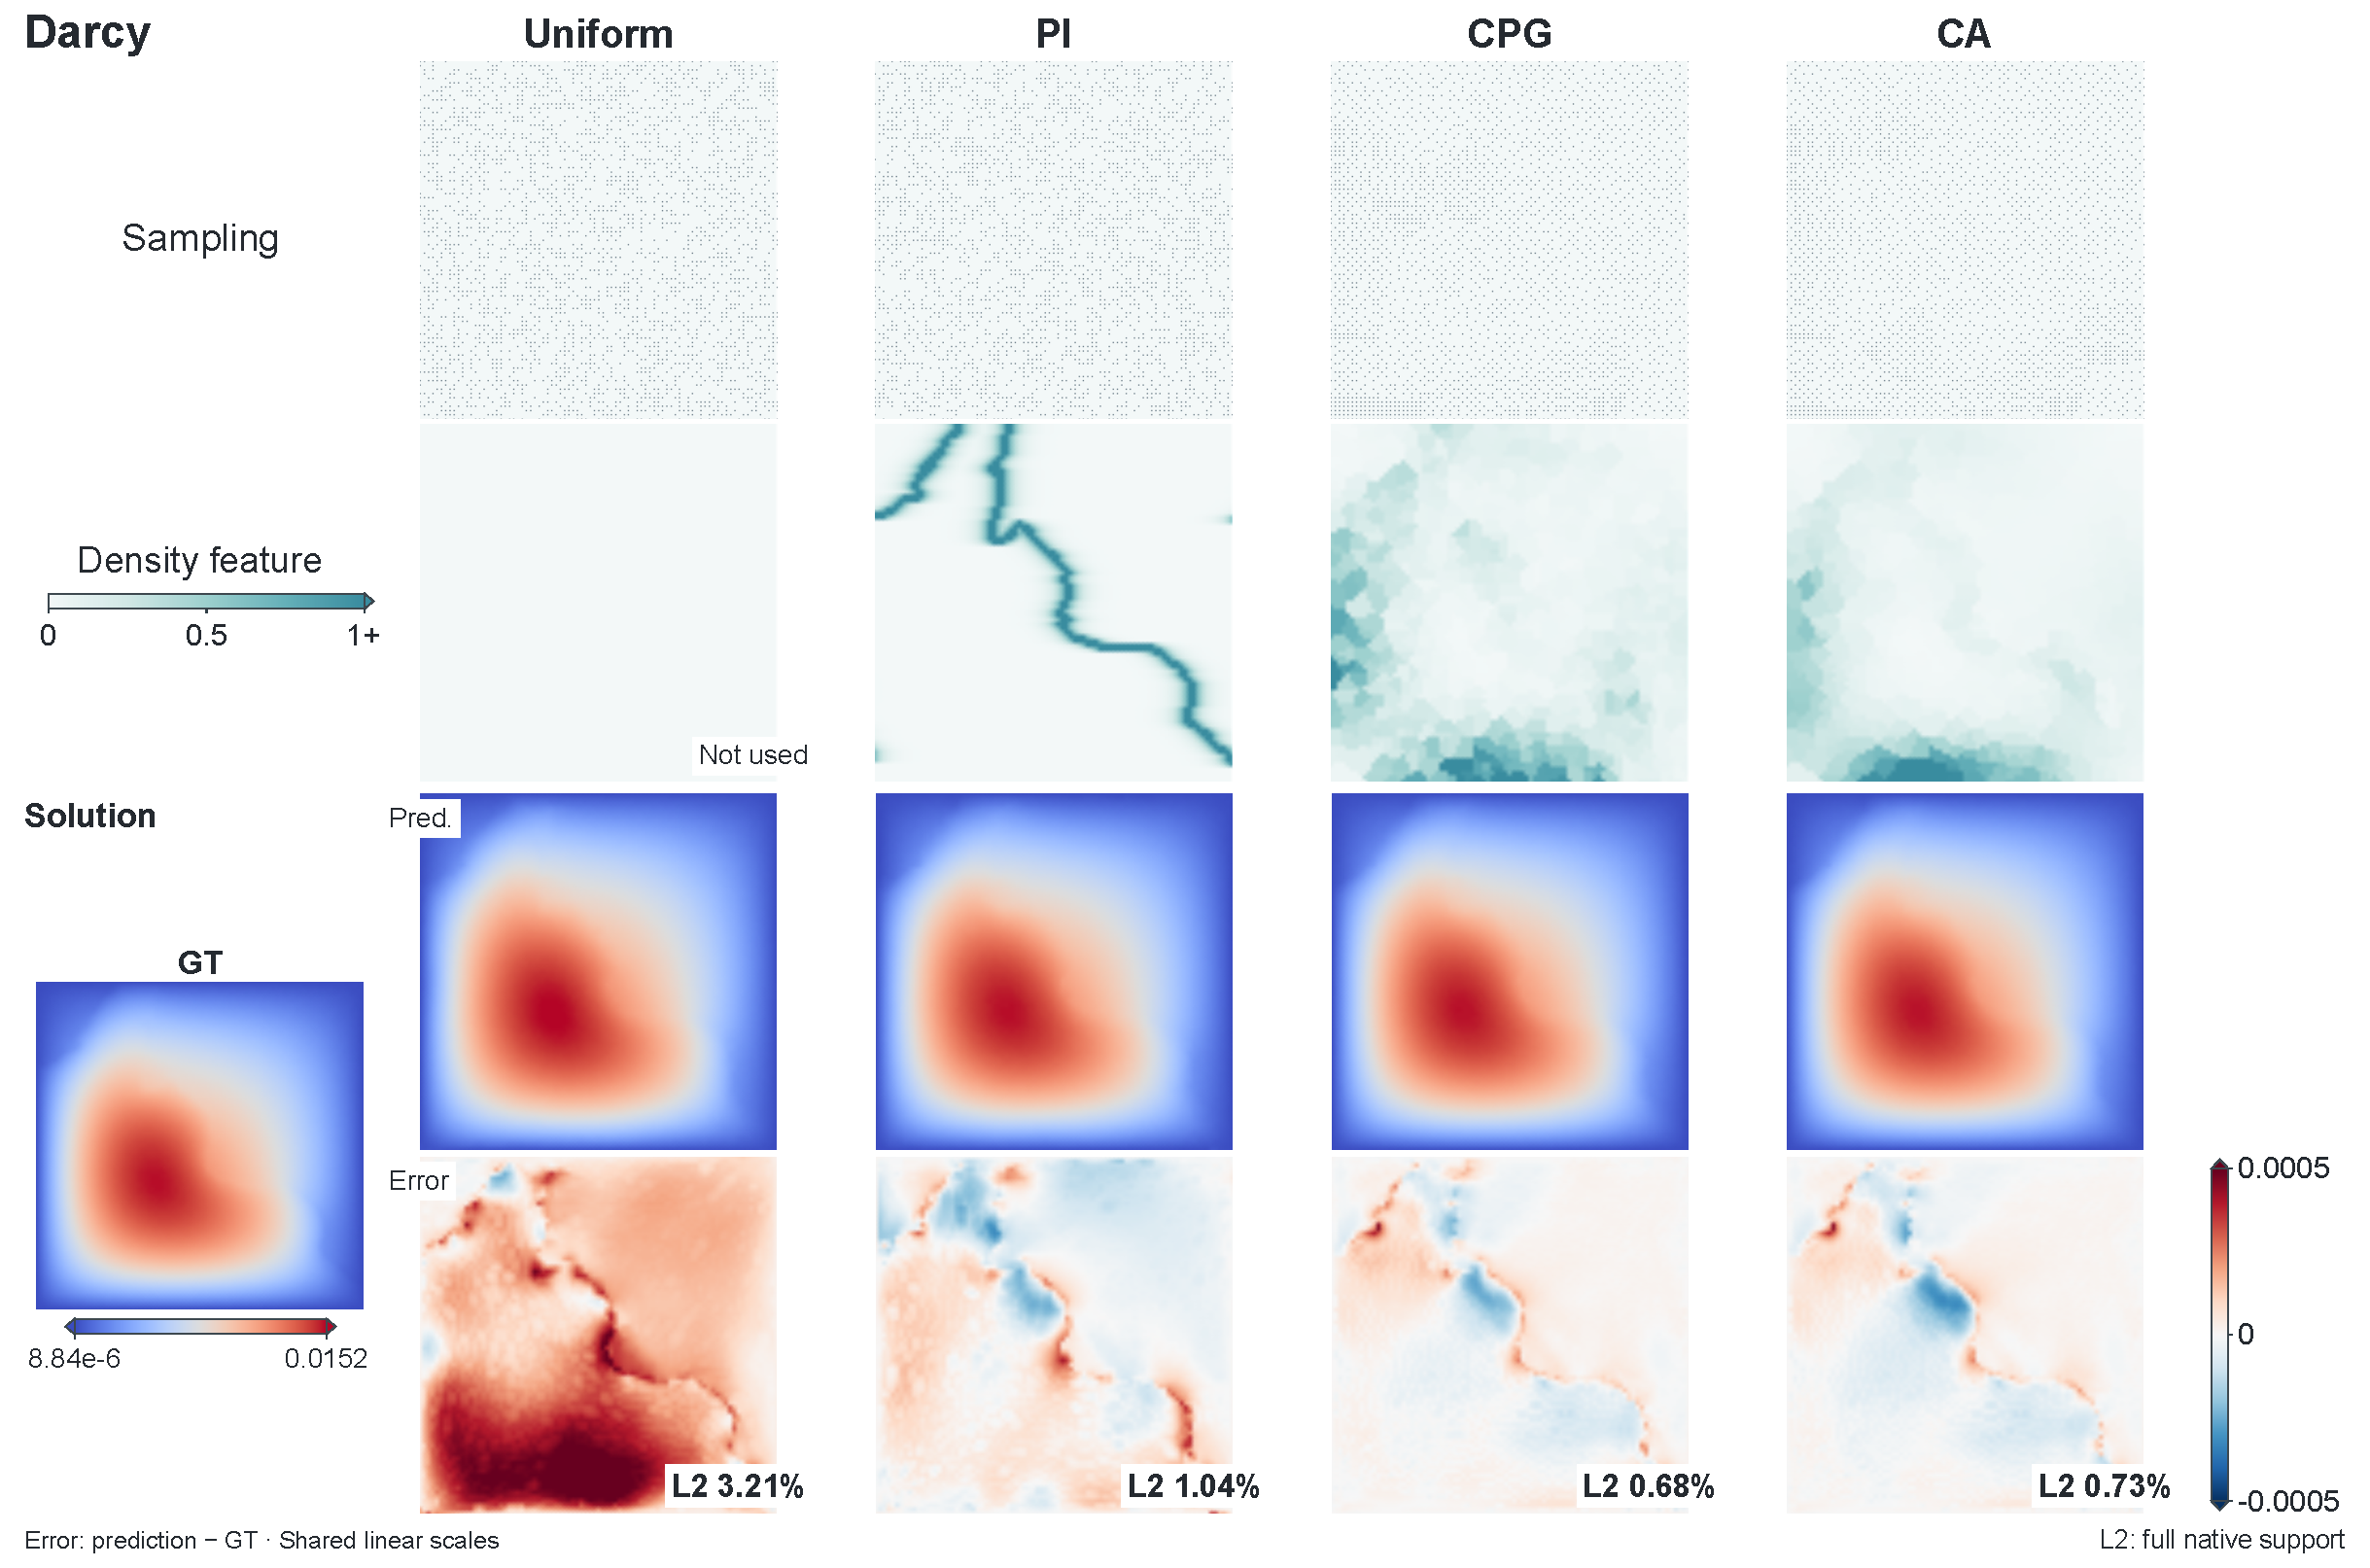
\includegraphics[width=\linewidth,height=.69\textheight,keepaspectratio]{figures/appendix/darcy_fields.pdf}
    \caption{\textbf{Darcy.} Sampling and pressure prediction.}
    \label{fig:appendix_darcy}
\end{figure}

\clearpage
\subsubsection{Elasticity}
\label{app:vis_elasticity}

The irregular hole creates localized stress structure. The residual views
show the reduction in reconstruction error around this region under adaptive
sampling. CPG and CA attain similar errors, with PI also improving
substantially upon the uniform allocation.

\begin{figure}[!ht]
    \centering
    \DIFdelbeginFL %DIFDELCMD < 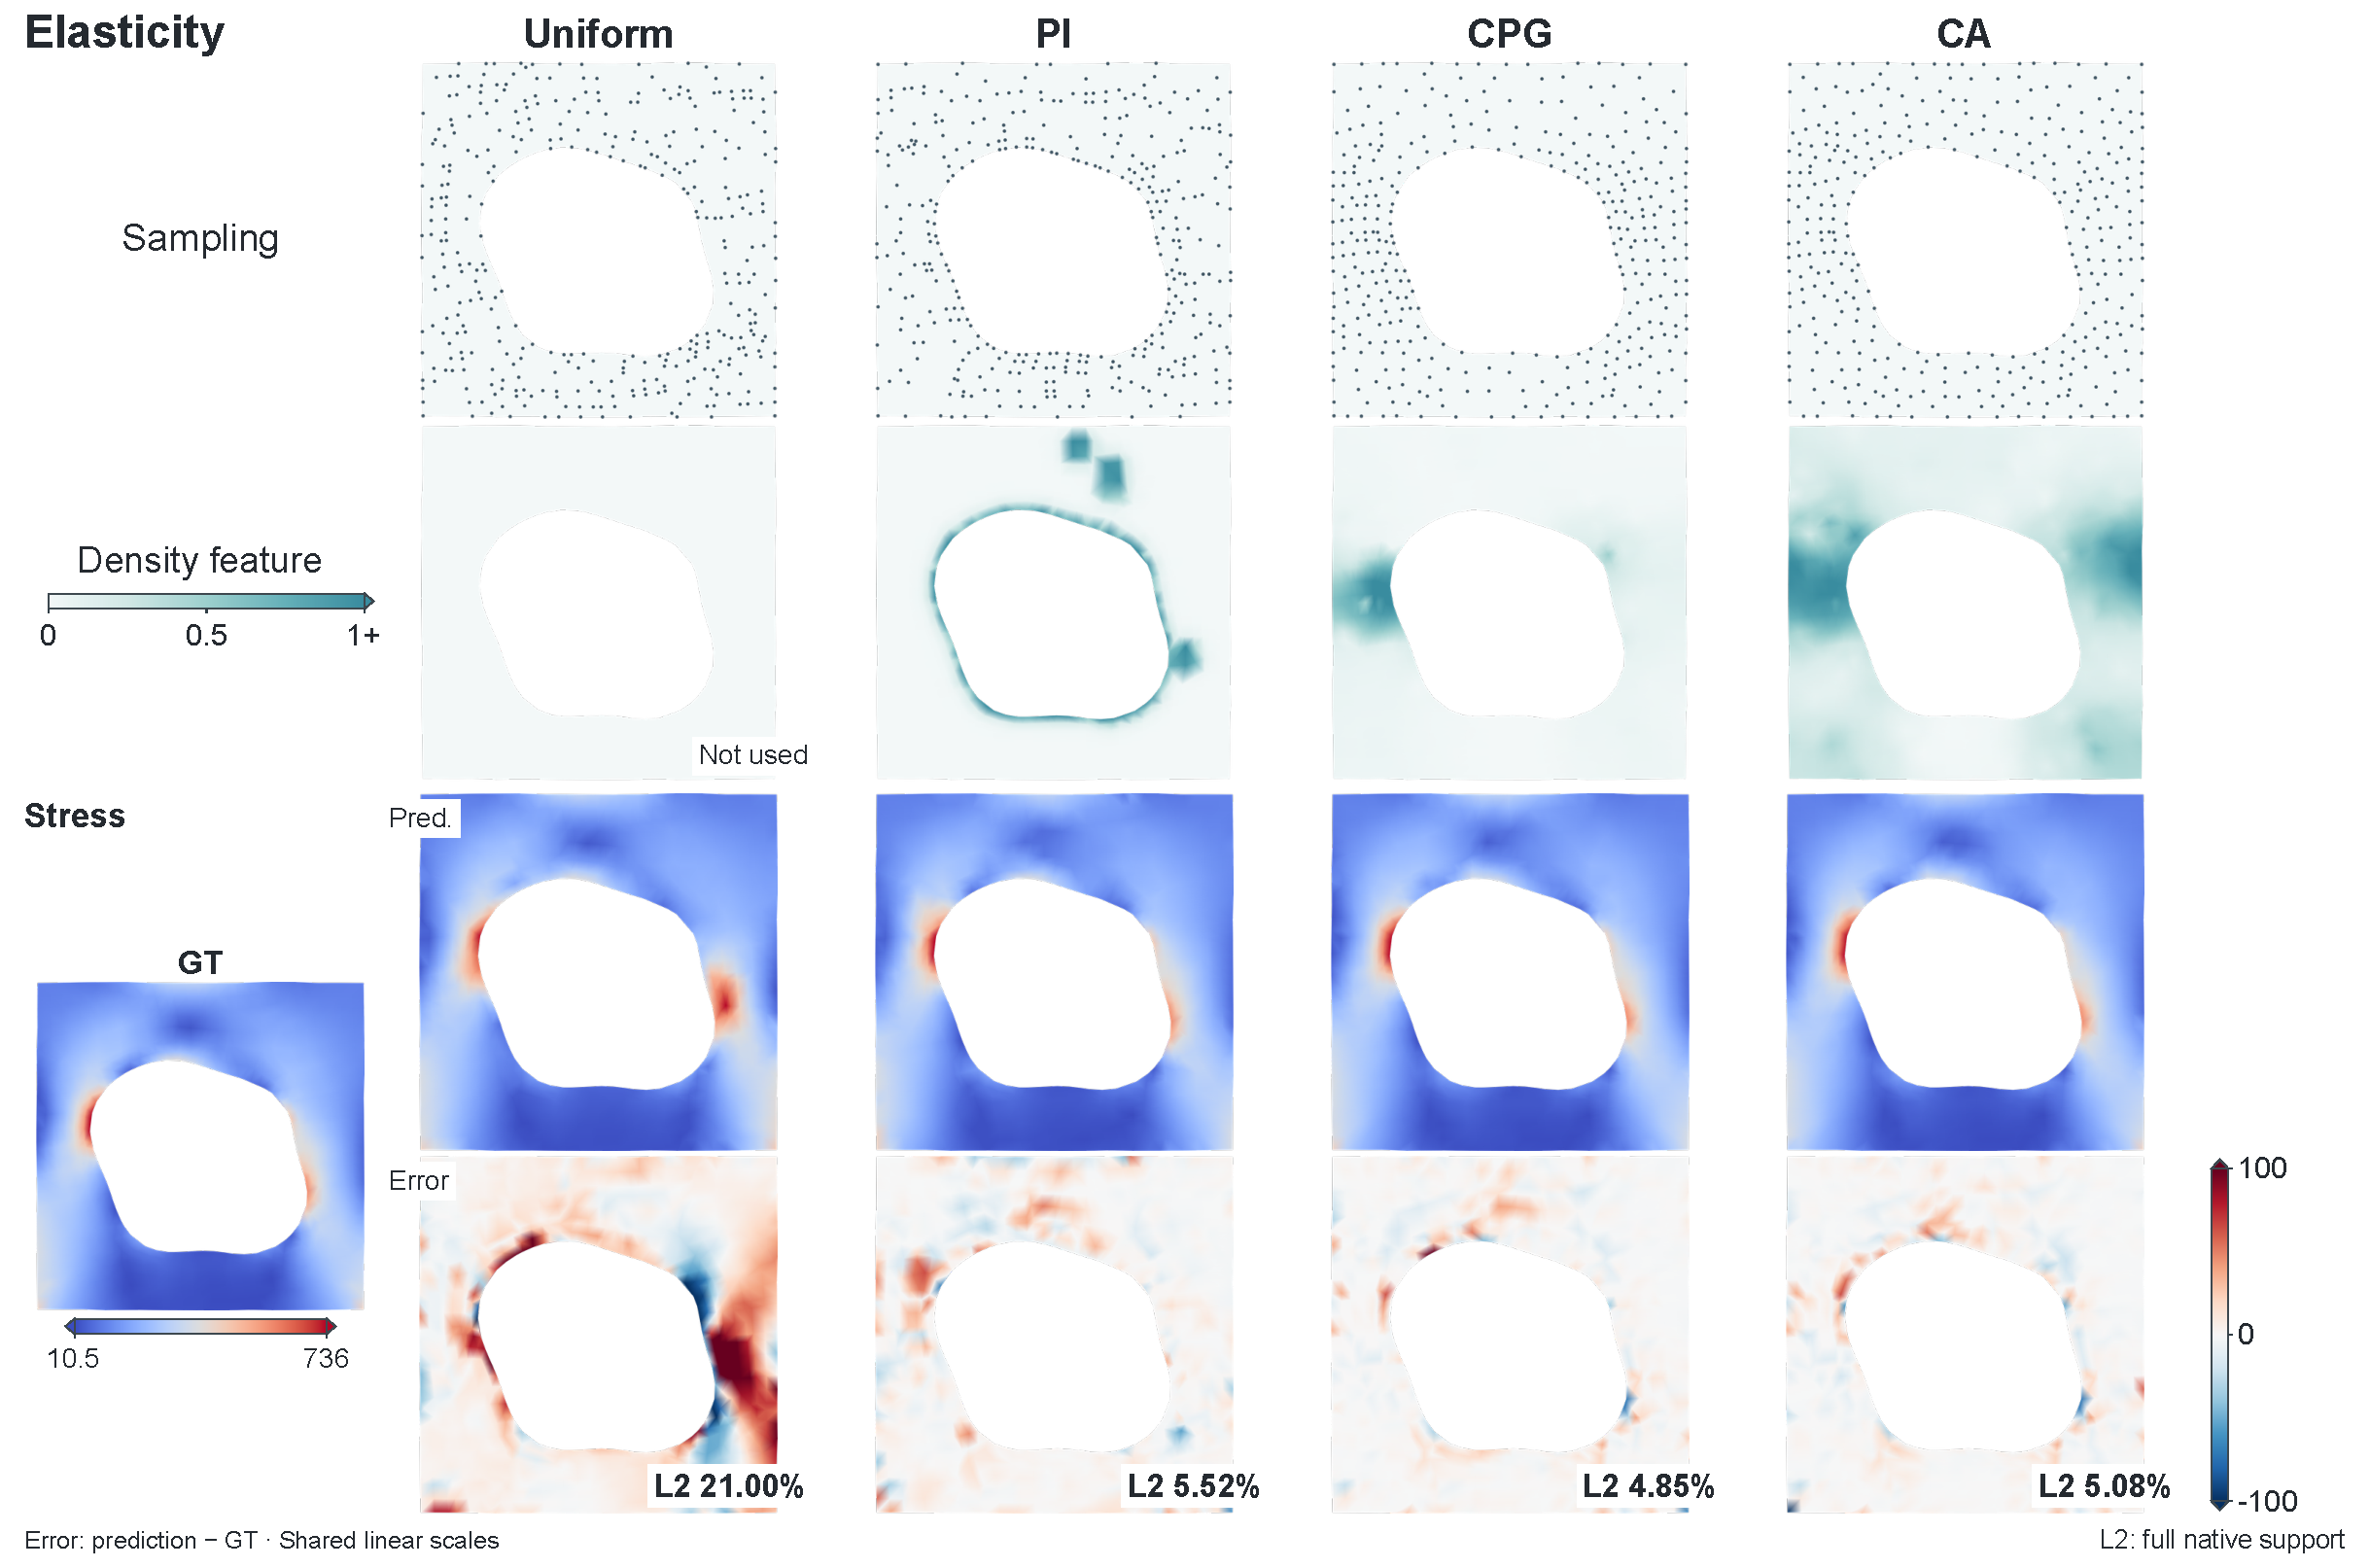
\includegraphics[width=\linewidth,height=.69\textheight,keepaspectratio]{review_assets/baseline/d4021228aa183f7d5f7912124d17d3f69f8930b9/figures/appendix/elasticity_fields.pdf}
%DIFDELCMD <     %%%
\DIFdelendFL \DIFaddbeginFL 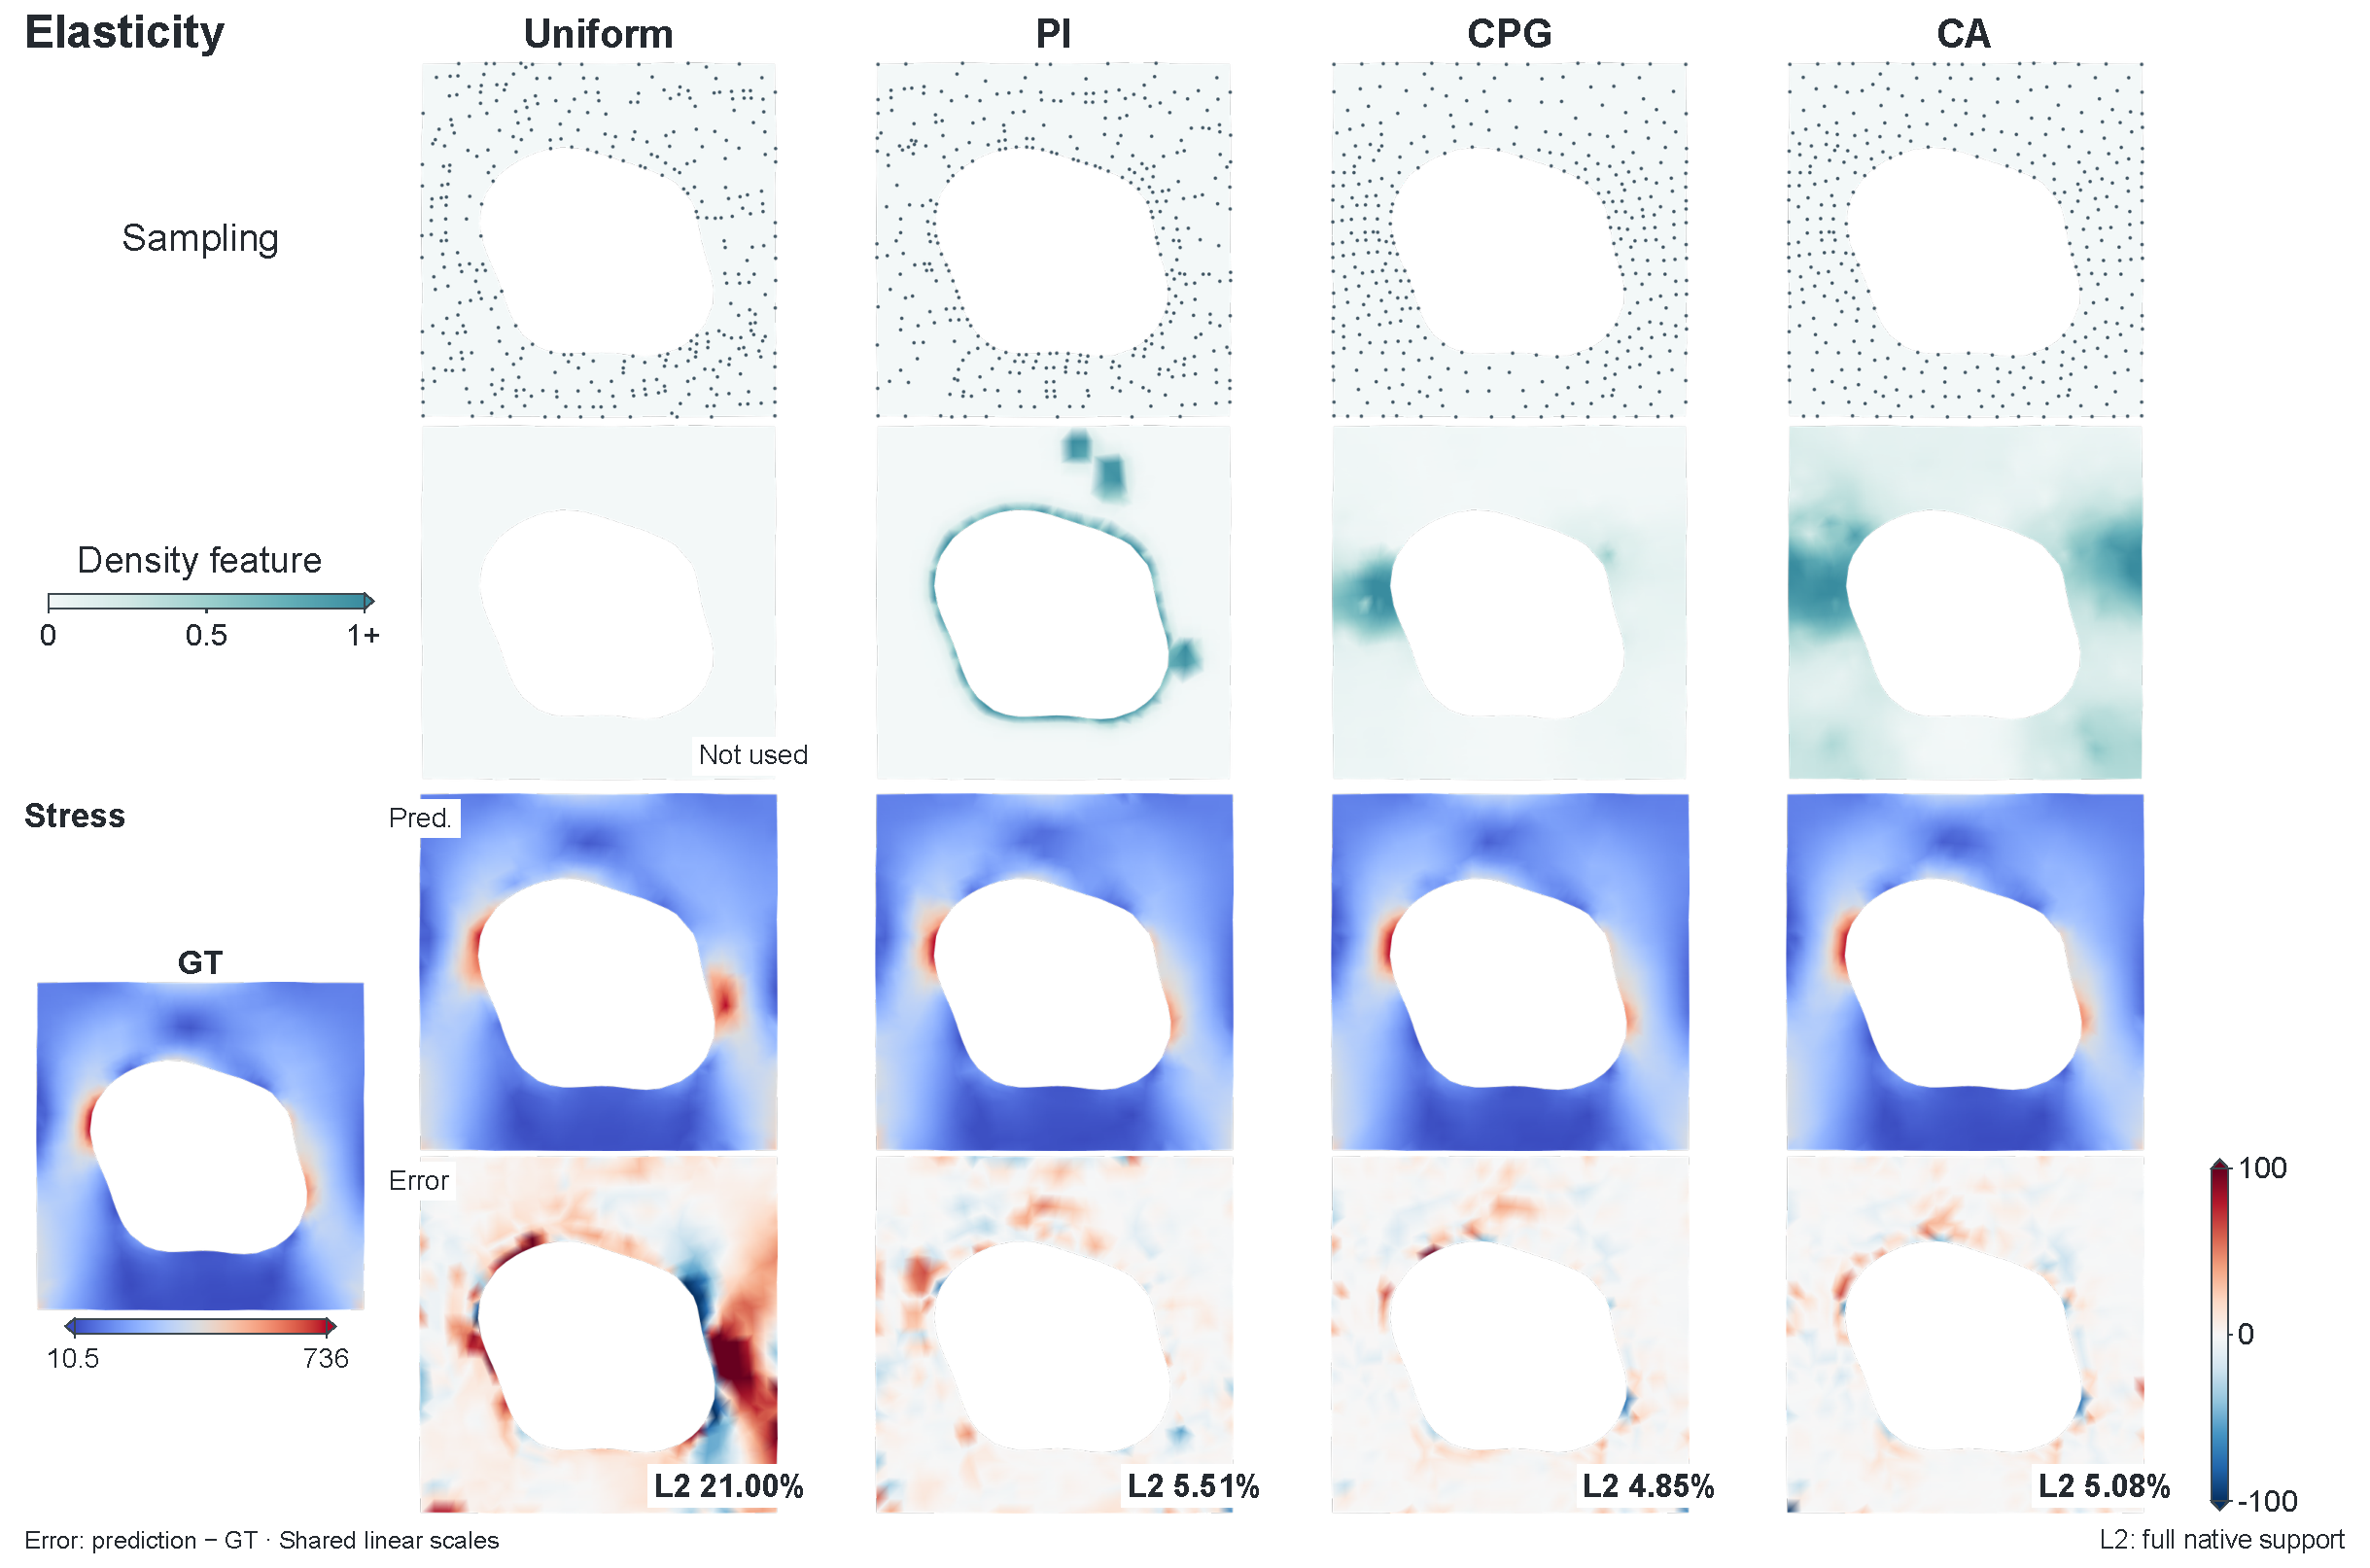
\includegraphics[width=\linewidth,height=.69\textheight,keepaspectratio]{figures/appendix/elasticity_fields.pdf}
    \DIFaddendFL \caption{\textbf{Elasticity.} Sampling and stress prediction.}
    \label{fig:appendix_elasticity}
\end{figure}

\clearpage
\subsubsection{Plasticity}
\label{app:vis_plasticity}

Plasticity predicts a sequence of 20 displacement fields. We summarize all
recorded steps with equal weights, $w_t=1/20$, because the time grid is
uniform. The field rows show time-averaged components and displacement
magnitude. Component-error rows average the absolute residual at each step.
The magnitude-error row averages the vector residual norm. The annotated
$L_2$ errors use the weighted space--time fields over all 20 steps.

\begin{figure}[!ht]
    \centering
    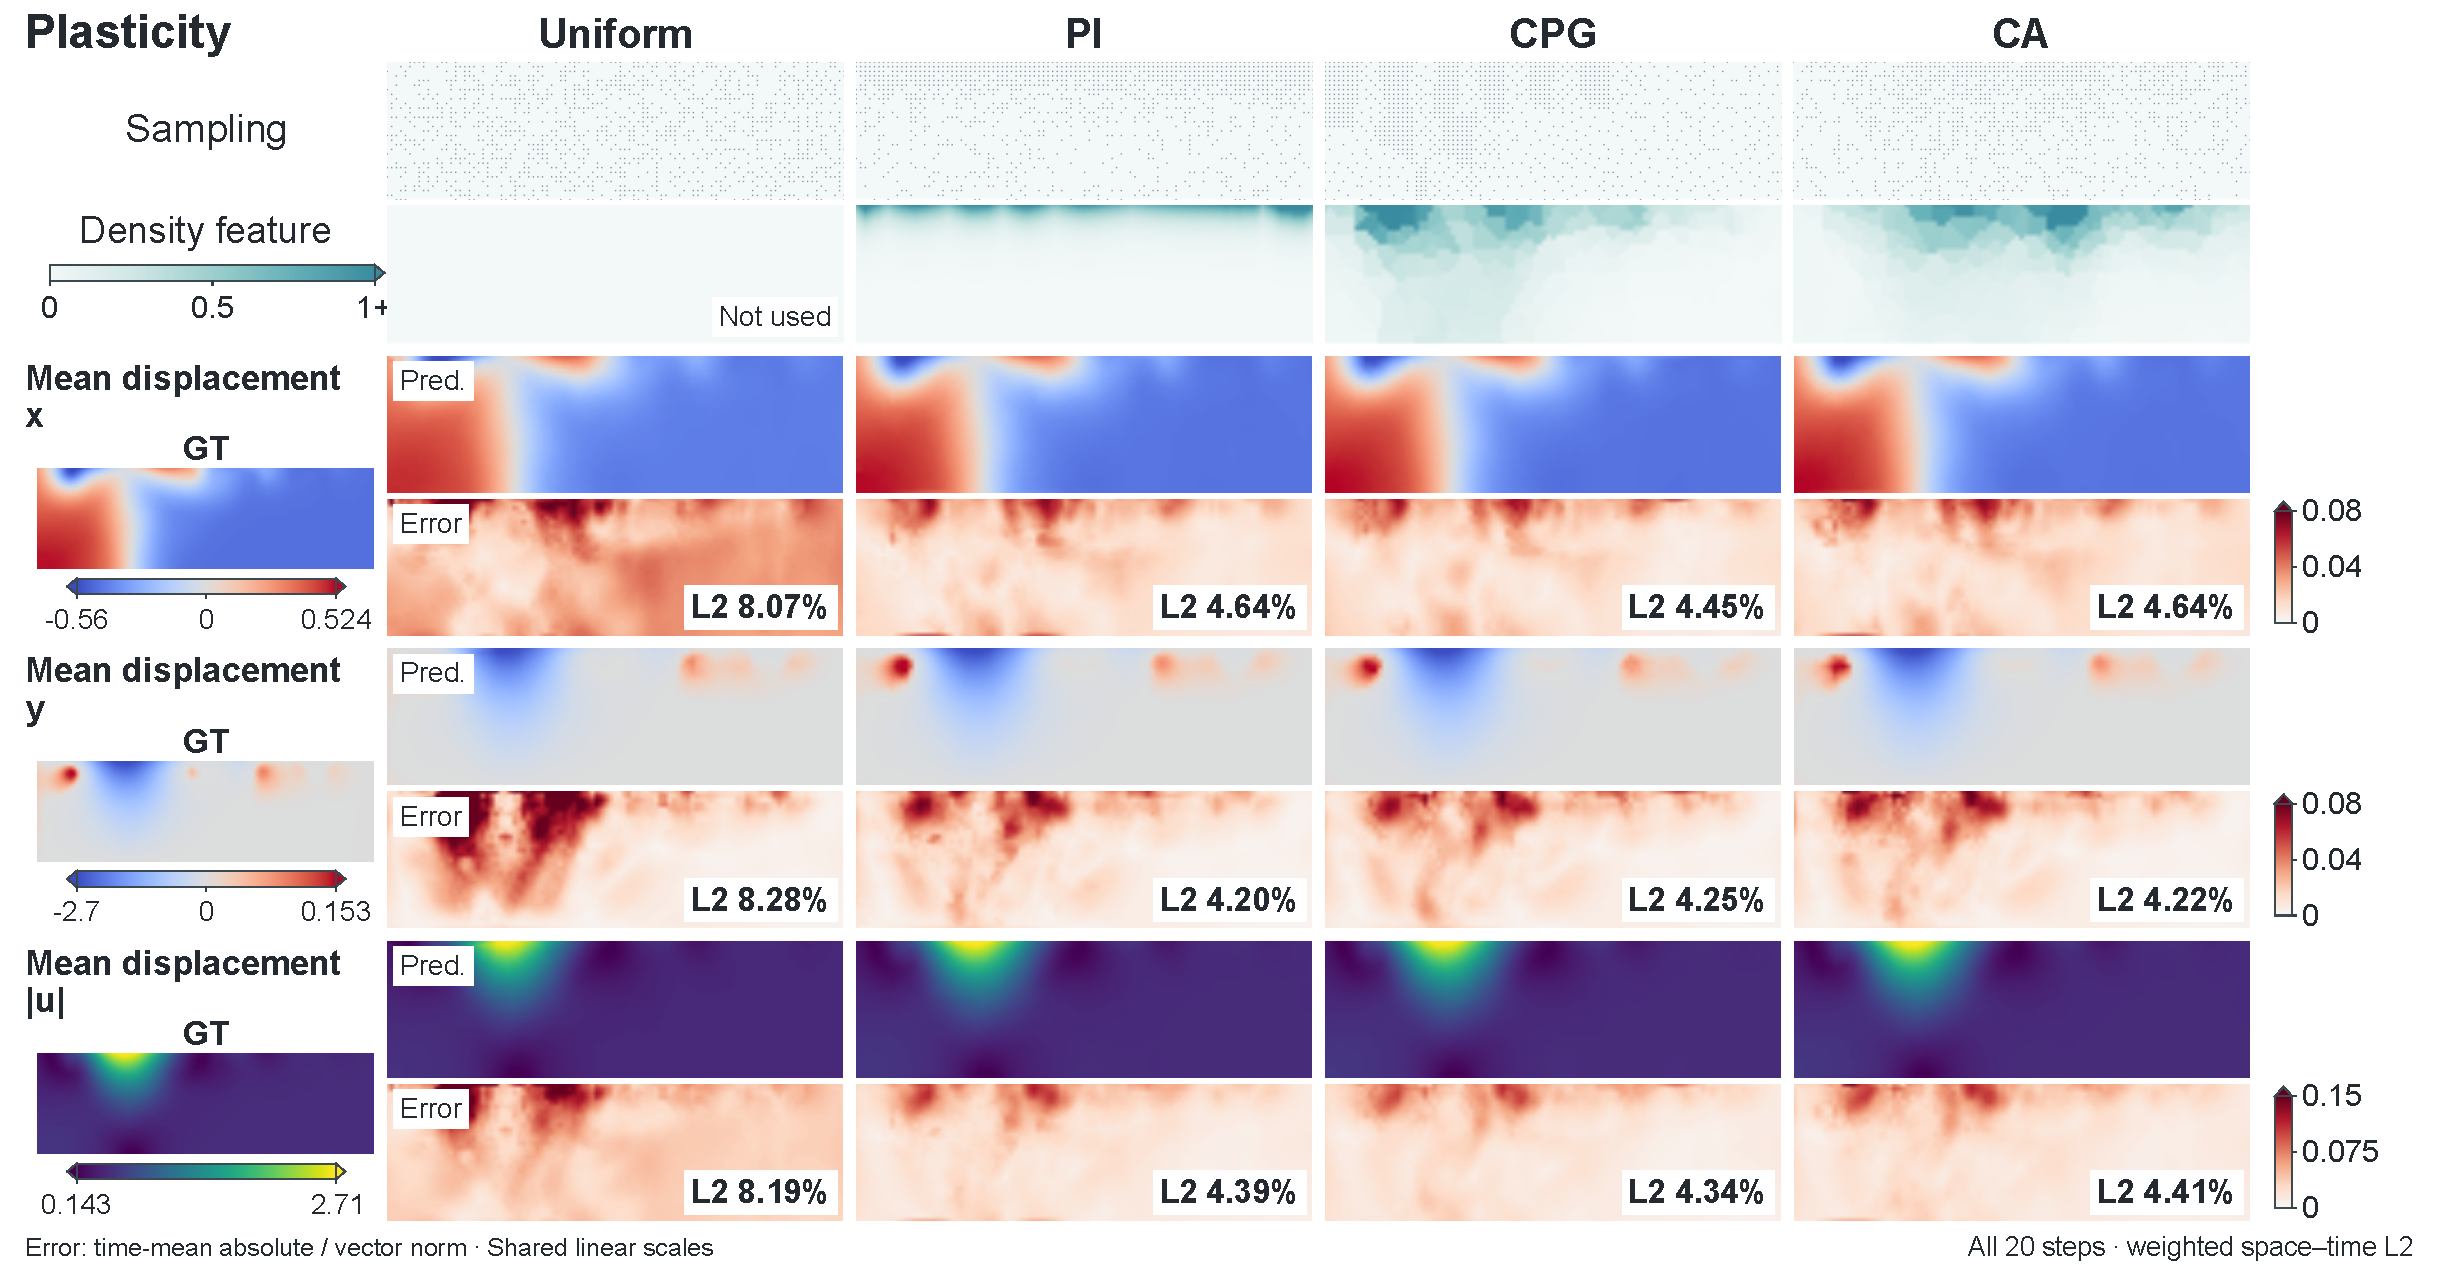
\includegraphics[width=\linewidth,height=.69\textheight,keepaspectratio]{figures/appendix/plasticity2d_fields.pdf}
    \caption{\textbf{Plasticity.} Sampling and displacement prediction.}
    \label{fig:appendix_plasticity}
\end{figure}

\clearpage
\subsubsection{ShapeNet-Car}
\label{app:vis_shapenet}

The automotive examples contain both surface and volumetric outputs.
For ShapeNet-Car, pressure is shown on the surface, and a fixed geometric
slice exposes the three velocity components and speed in the surrounding
volume. Error annotations use each field's full native support. This view
connects changes in point allocation to both pressure and velocity accuracy.

\begin{figure}[!ht]
    \centering
    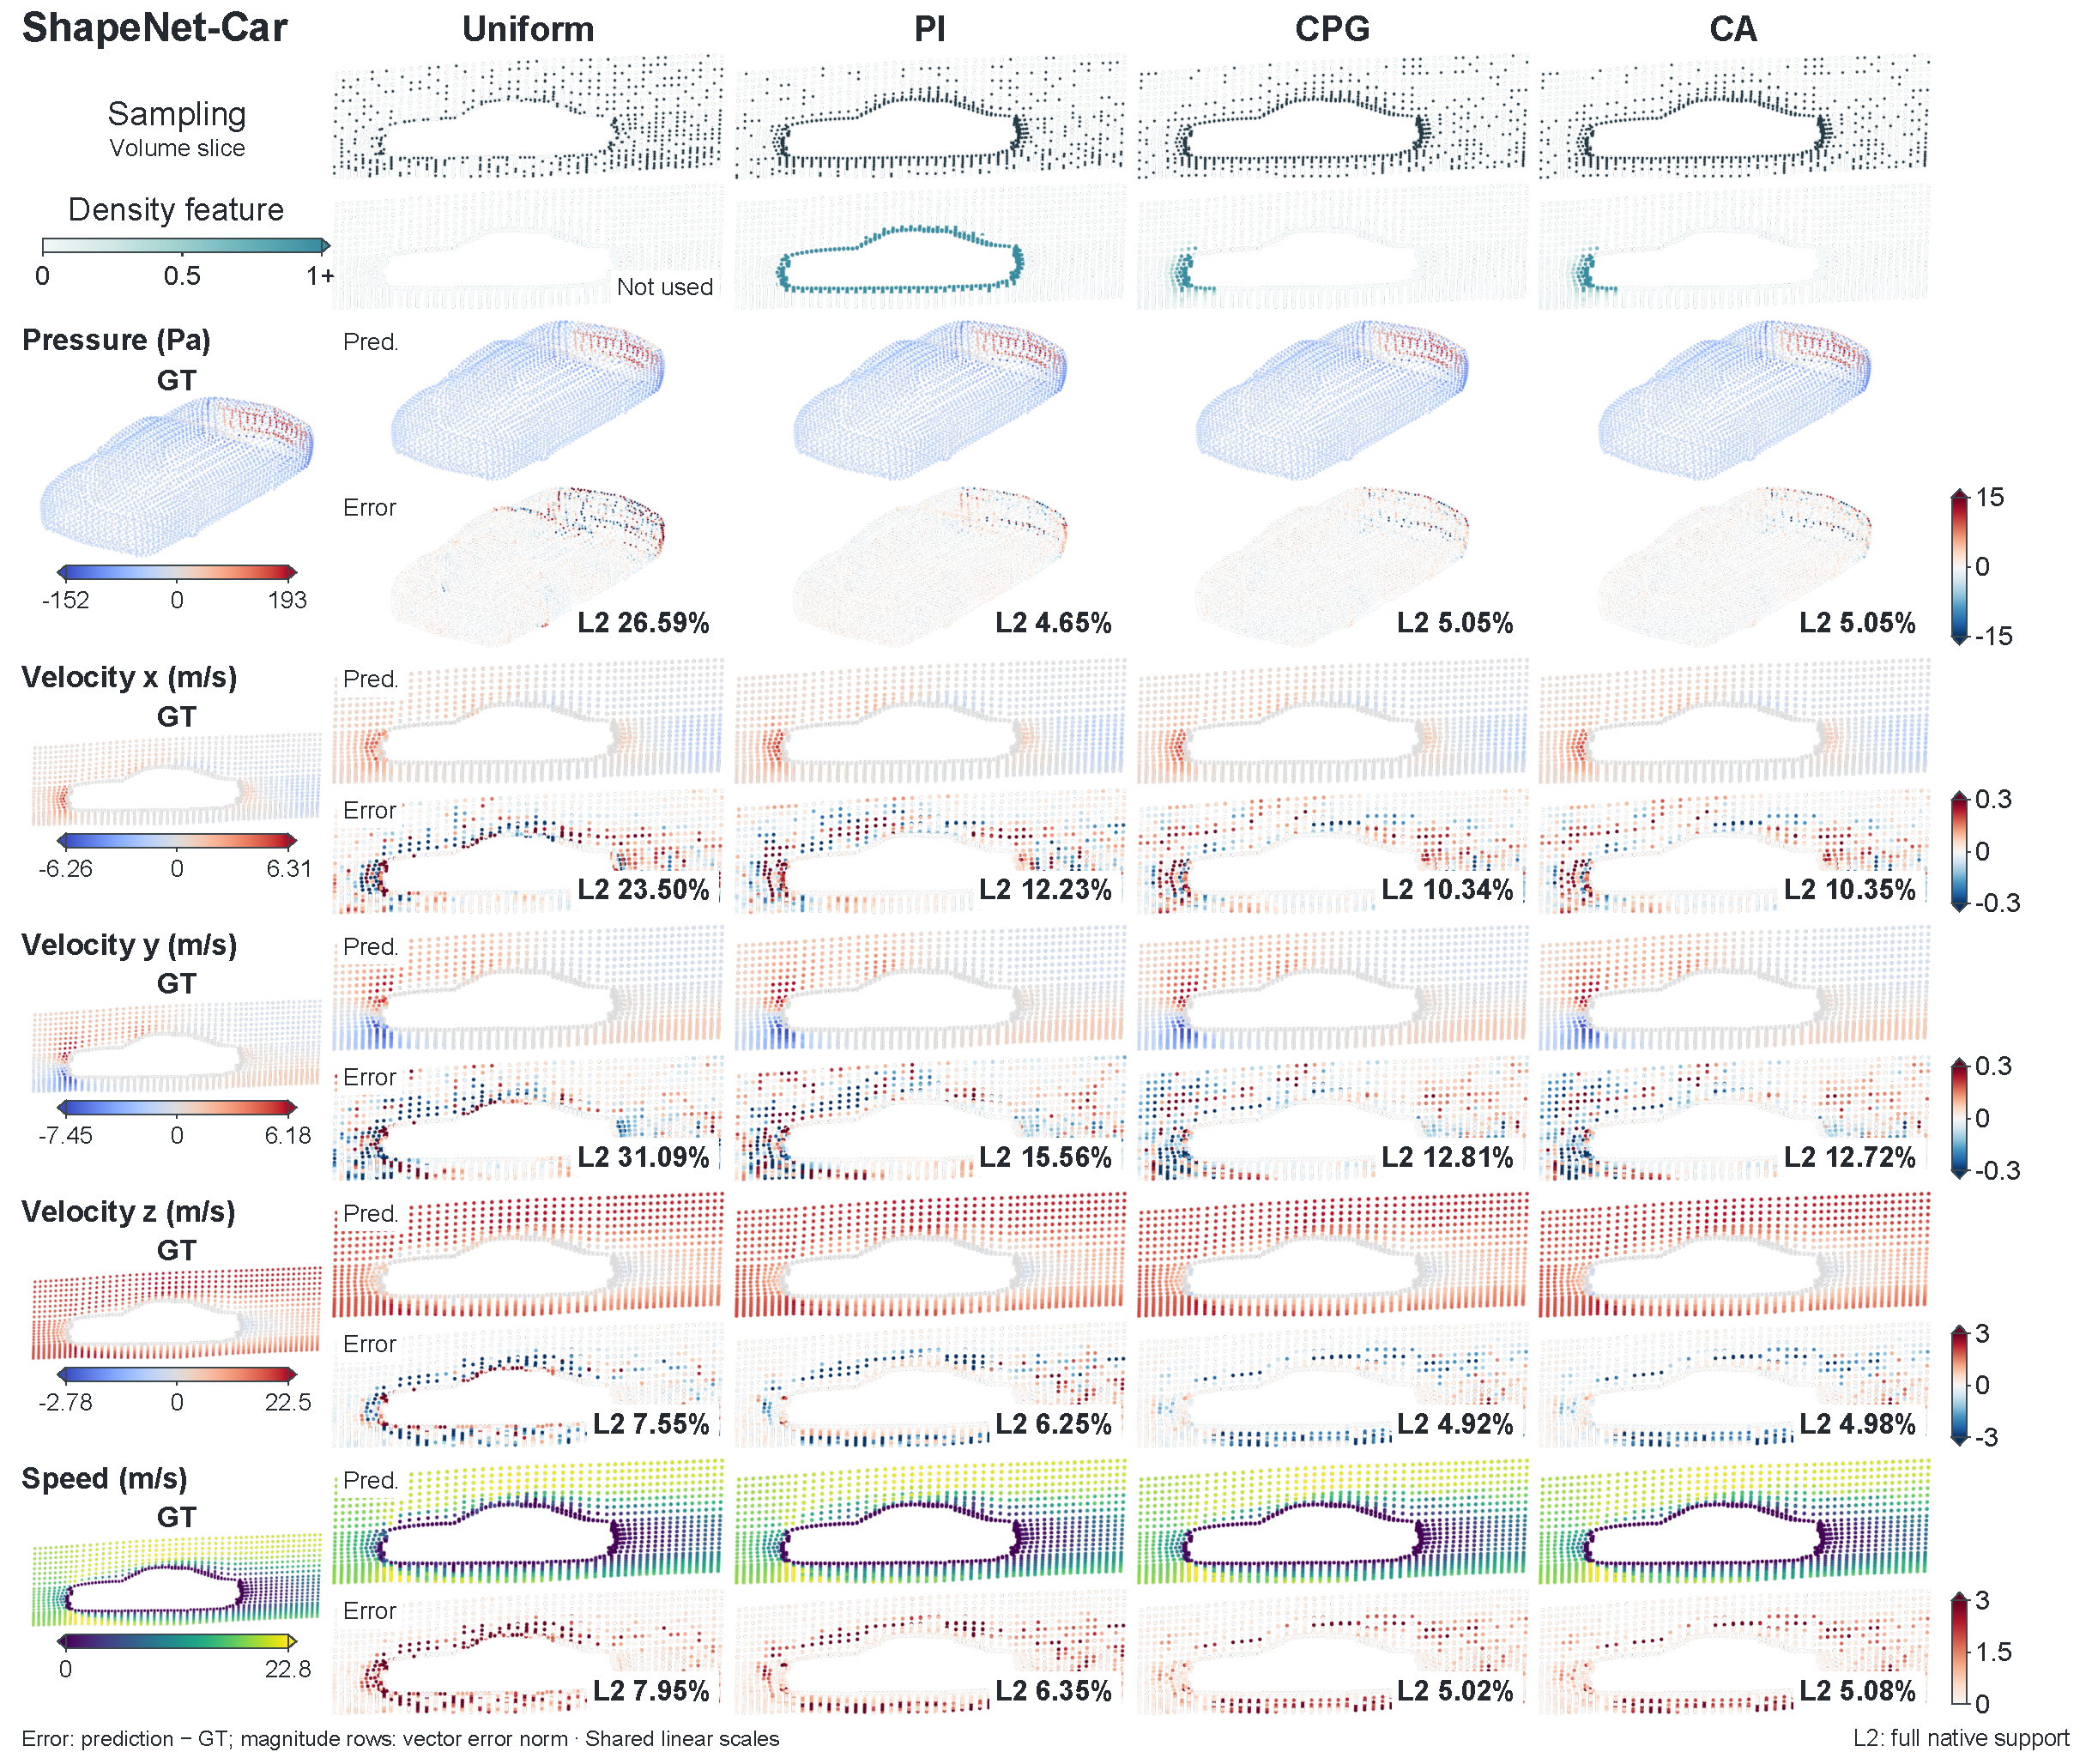
\includegraphics[width=\linewidth,height=.69\textheight,keepaspectratio]{figures/appendix/shapenet_car_fields.pdf}
    \caption{\textbf{ShapeNet-Car.} Sampling and prediction of surface pressure
    and volumetric velocity.}
    \label{fig:appendix_shapenet}
\end{figure}

\clearpage
\subsubsection{DrivAerML}
\label{app:vis_drivaer}

DrivAerML provides pressure and wall-shear-stress predictions on the same
vehicle surface. We reuse each pressure sampler's point indices for the
frozen wall-shear-stress operator. The figure therefore shows how these
allocations affect pressure, all three shear components, and their vector
magnitude on a shared geometry.

\begin{figure}[!ht]
    \centering
    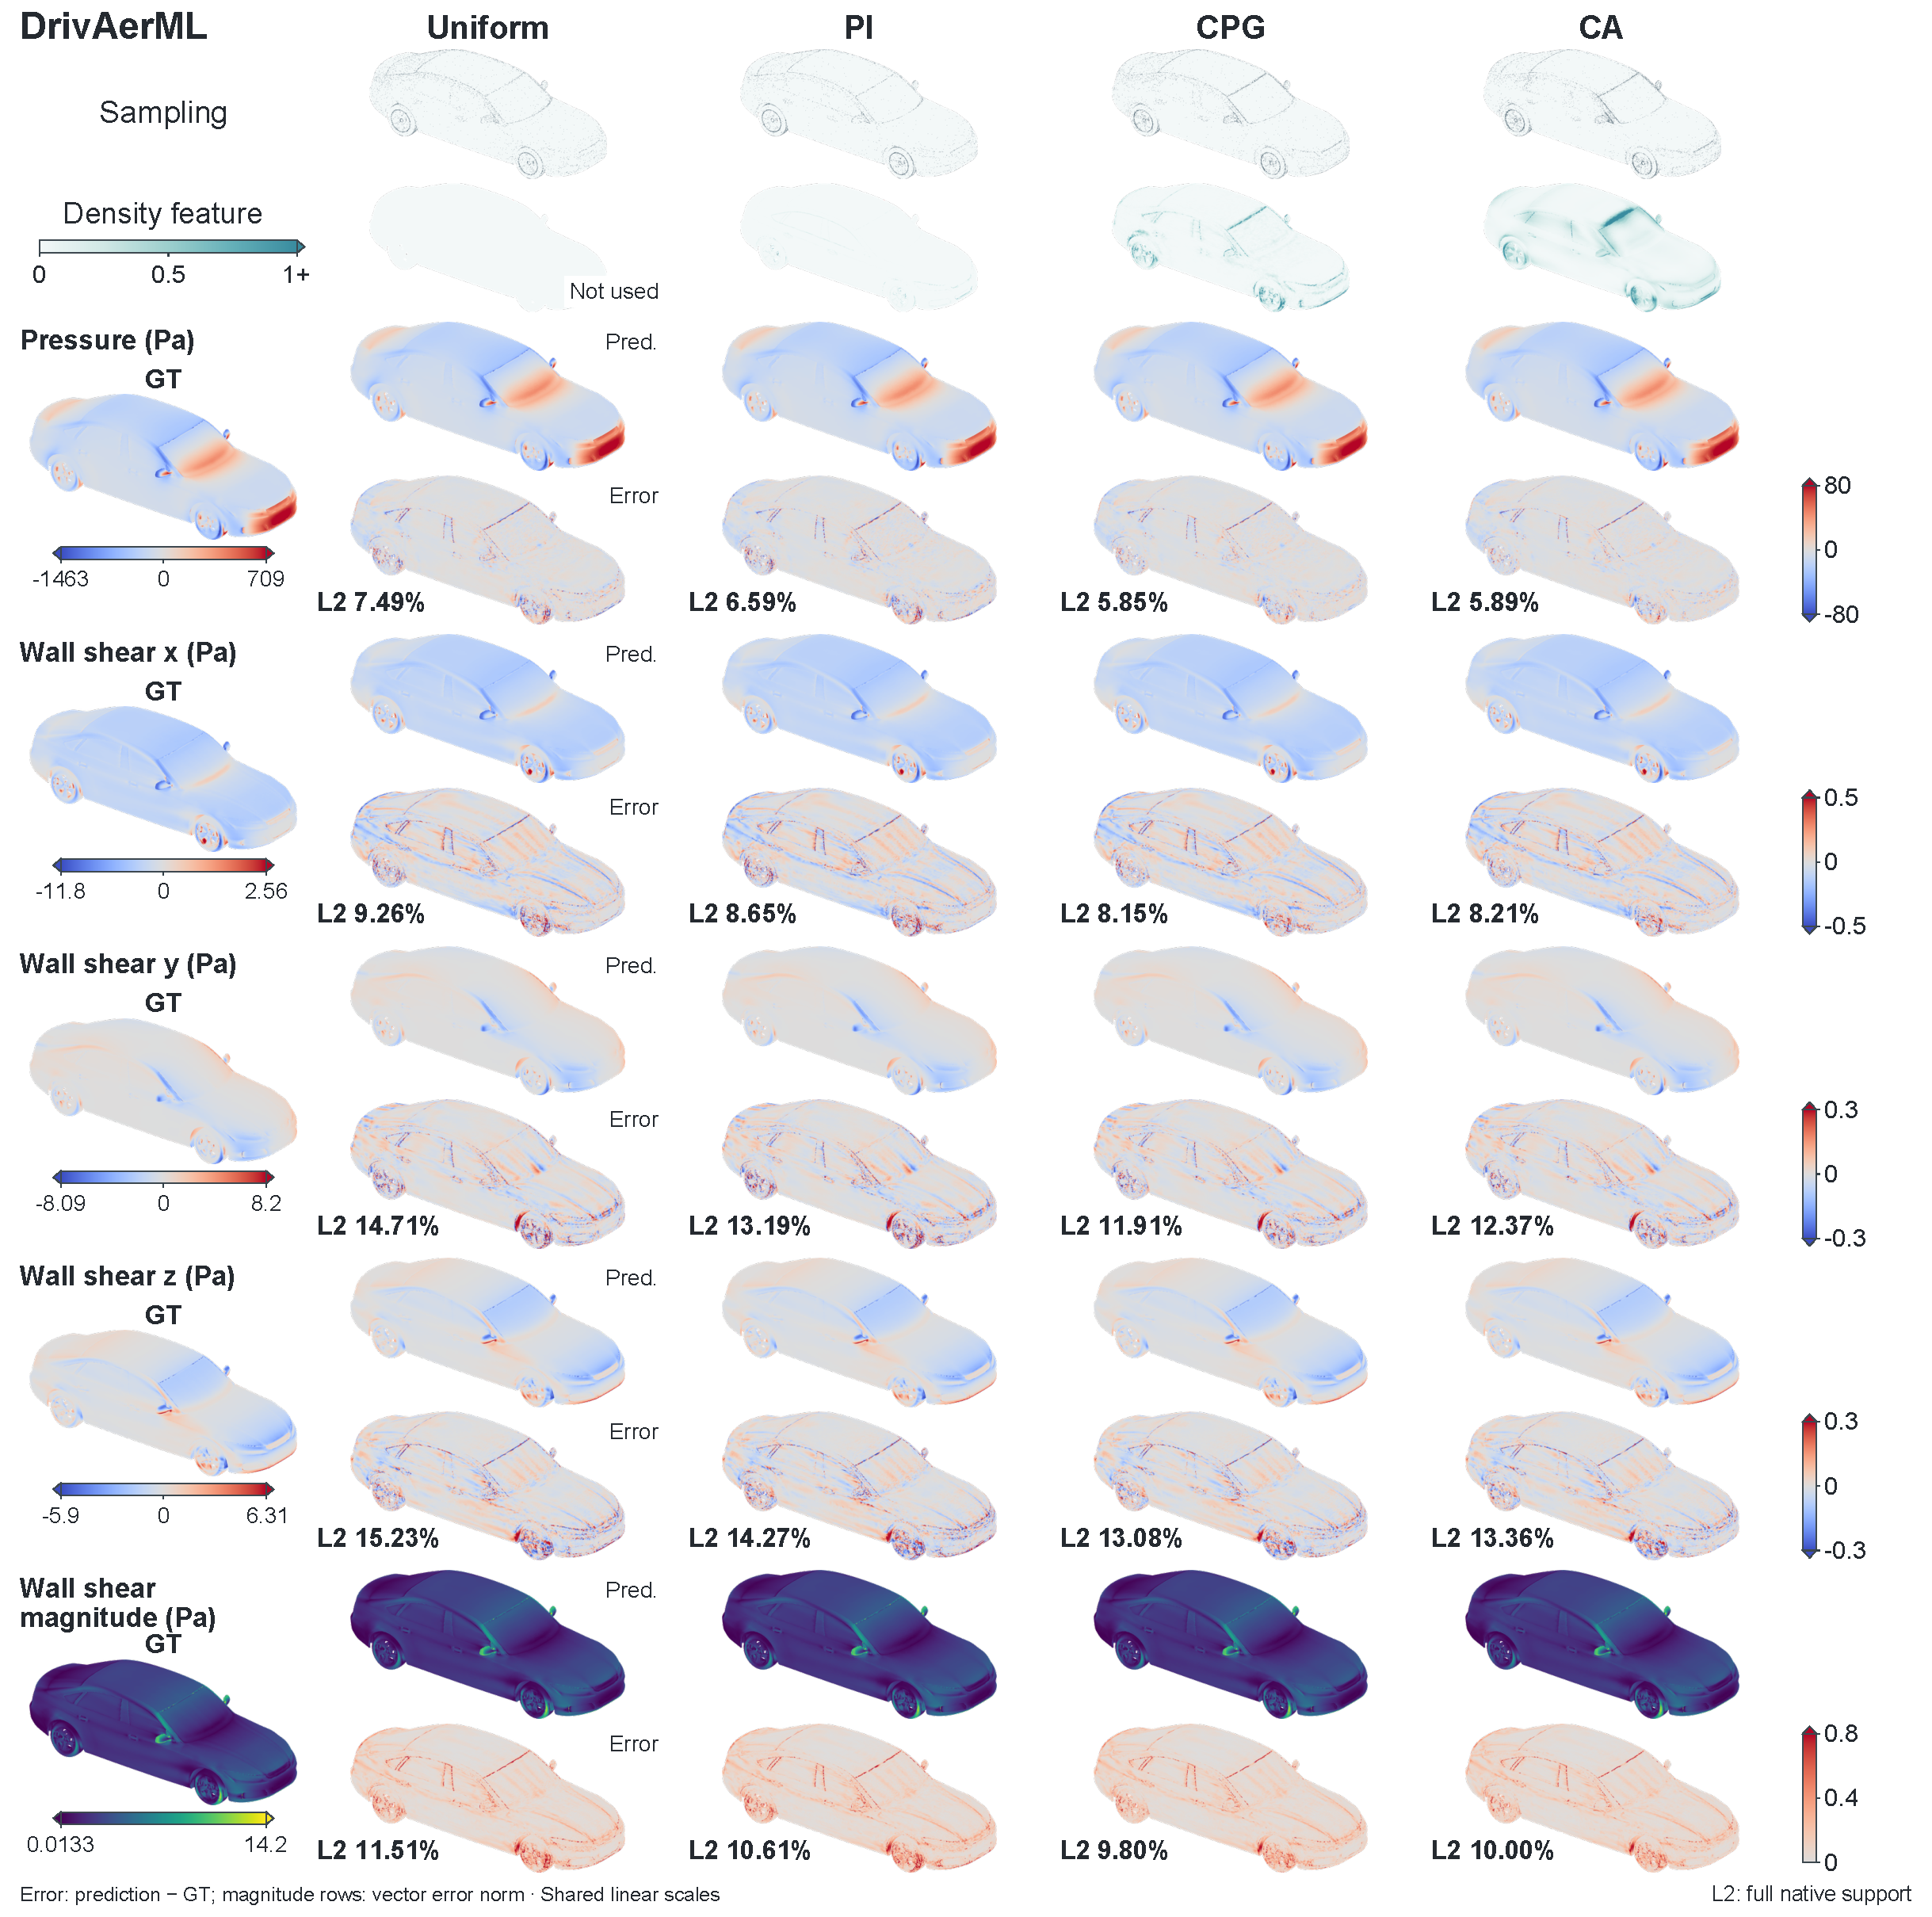
\includegraphics[width=\linewidth,height=.69\textheight,keepaspectratio]{figures/appendix/driverml_fields.pdf}
    \caption{\textbf{DrivAerML.} Sampling and prediction of surface pressure
    and wall shear stress.}
    \label{fig:appendix_drivaer}
\end{figure}

\clearpage
\subsubsection{SuperWing}
\label{app:vis_superwing}

The SuperWing page retains pressure and both friction components, together
with friction magnitude. The stored friction-channel scaling factors are
undone before visualization. Policy ordering varies across these outputs:
CPG gives the smallest pressure error for this wing, while PI gives the
smallest tangent-friction error. The individual rows expose this variation
beyond the joint field metric.

\begin{figure}[!ht]
    \centering
    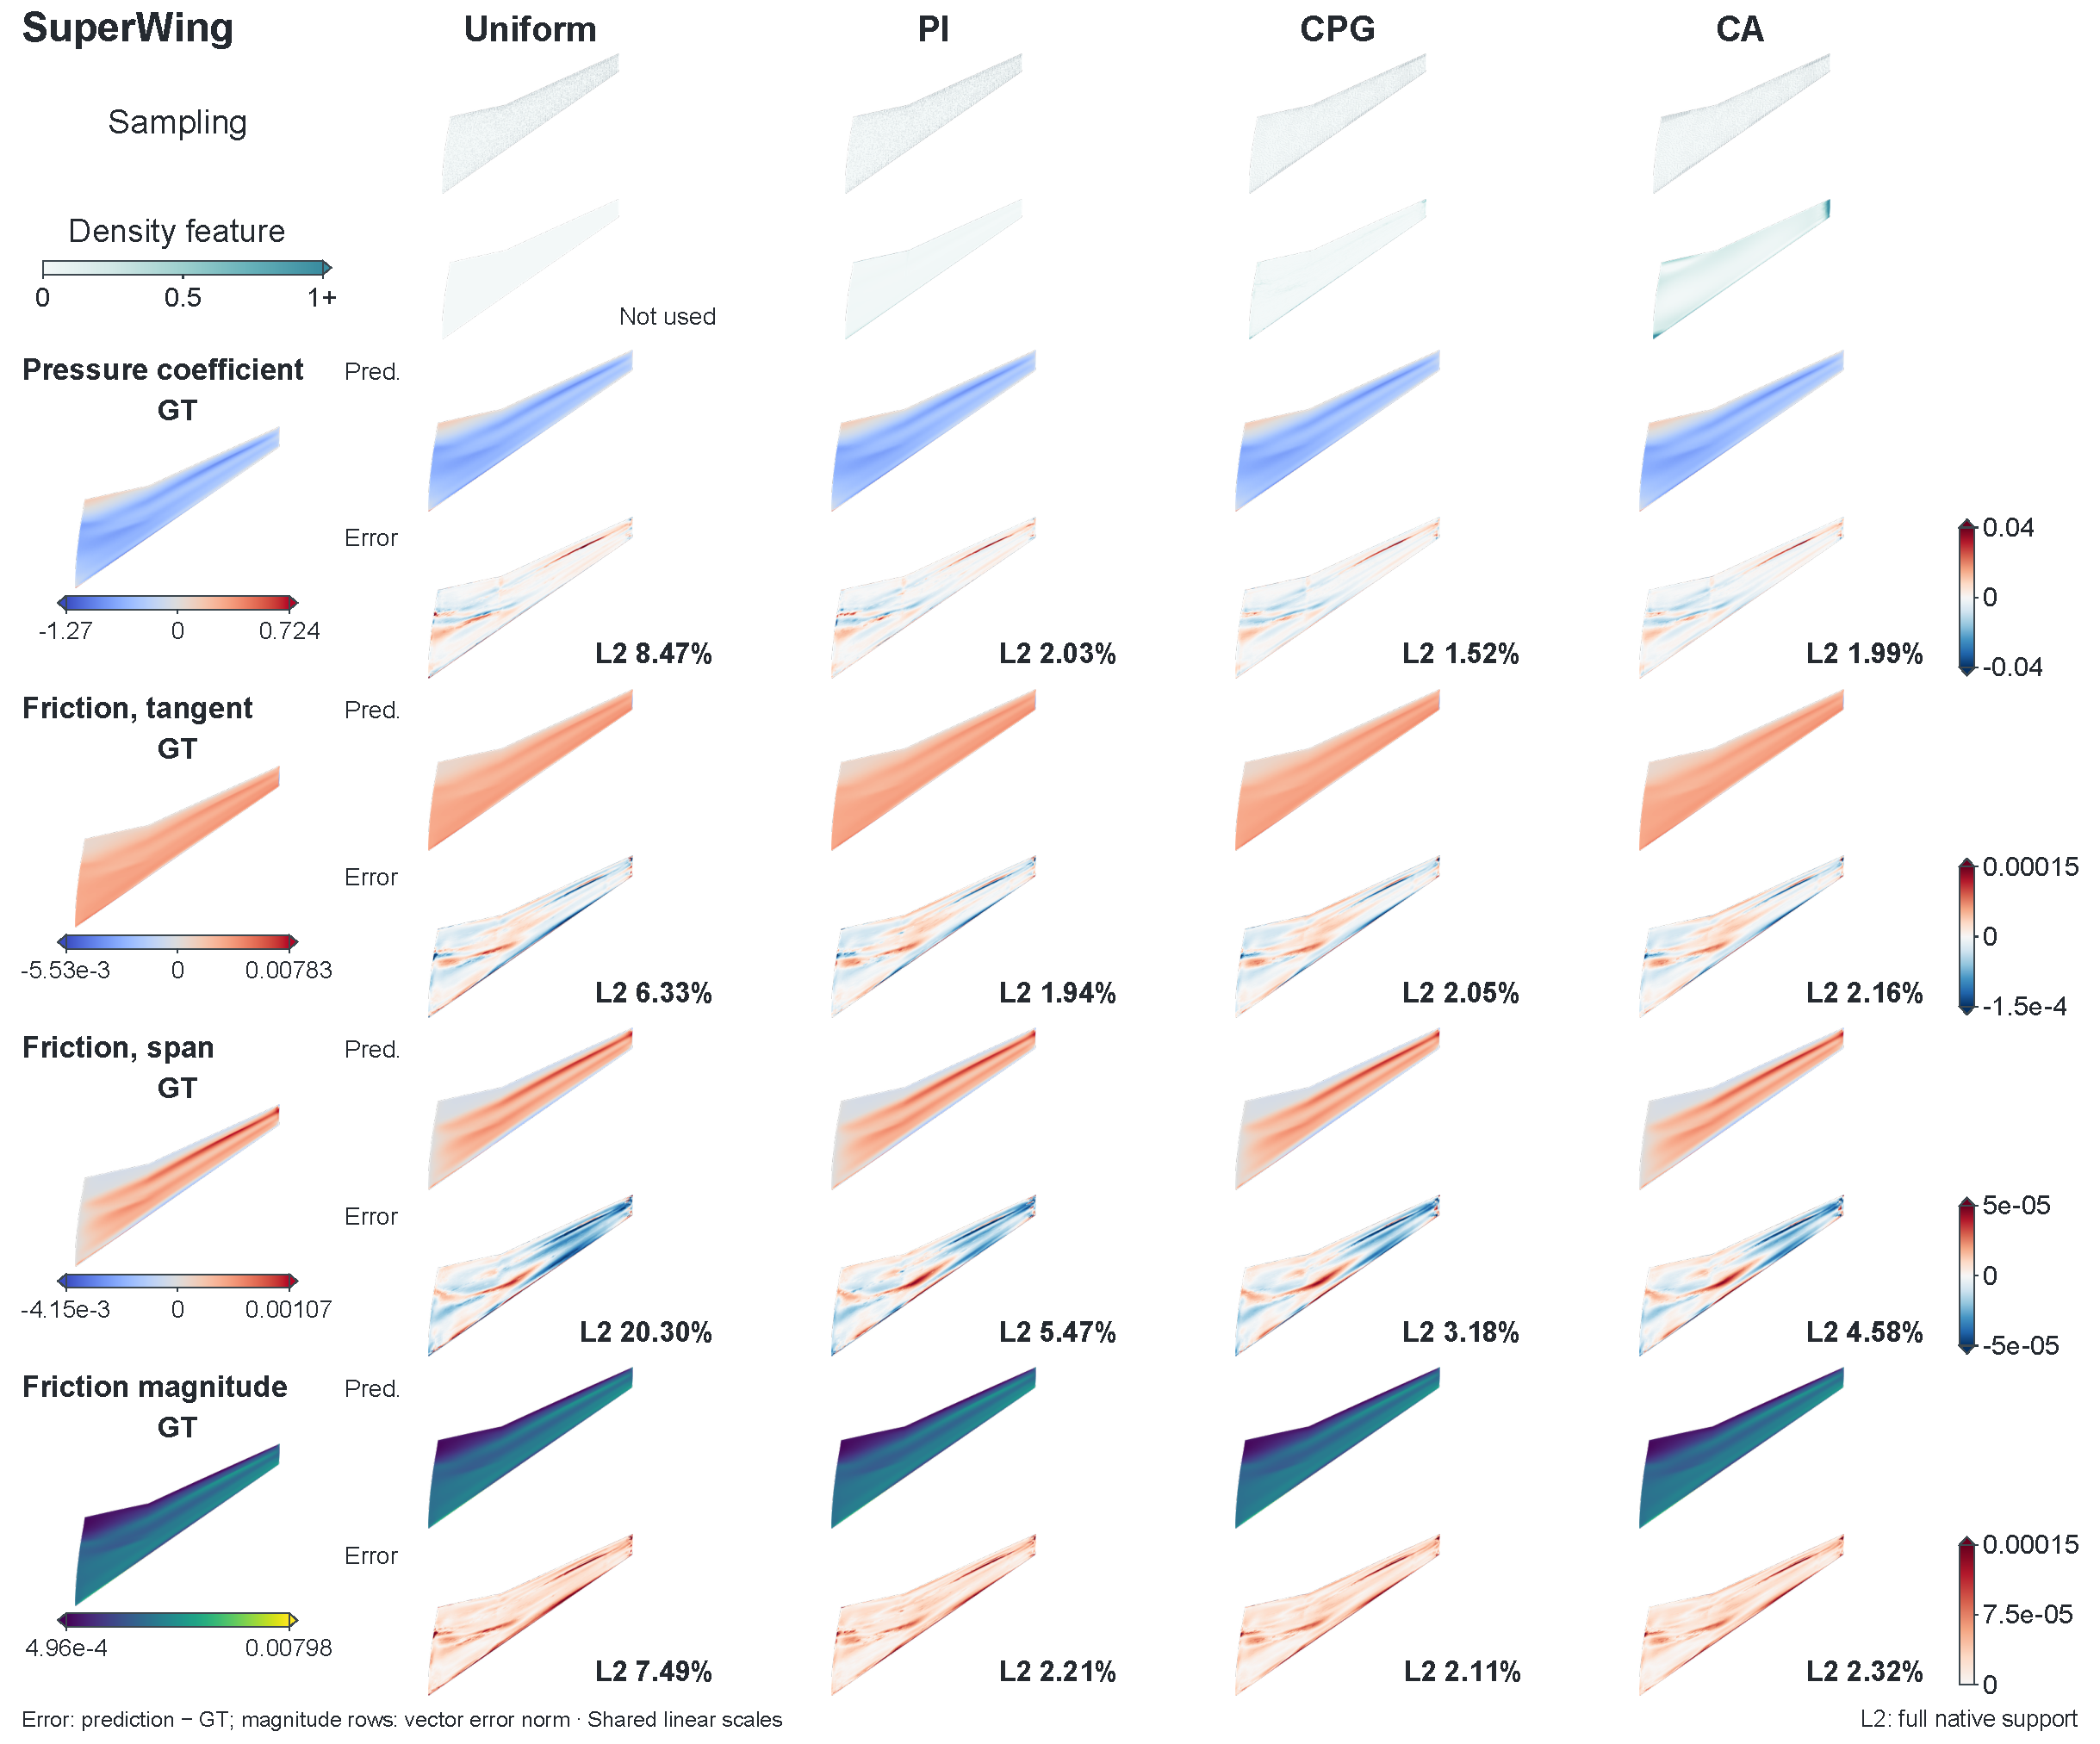
\includegraphics[width=\linewidth,height=.69\textheight,keepaspectratio]{figures/appendix/superwing_fields.pdf}
    \caption{\textbf{SuperWing.} Sampling and prediction of pressure
    and skin-friction coefficients.}
    \label{fig:appendix_superwing}
\end{figure}

\DIFaddbegin \clearpage
\subsection{\DIFadd{Refinement Score Visualization}}
\label{app:score_visualization}

\DIFadd{Figure~\ref{fig:appendix_refinement_scores} shows the spatial signals used
to construct the sampling policies. PI uses prior information, CPG uses
variation in a coarse prediction, and CA uses a predicted score or a
physical quantity from which the score is computed. For ShapeNet-Car,
the maps show the physical-body prior and the pressure-variation signals
of the Field policies; the full allocation also combines the near-wall
and wake terms specified in Appendix~\ref{app:density_policy_design}.
}

\begin{figure}[H]
    \centering
    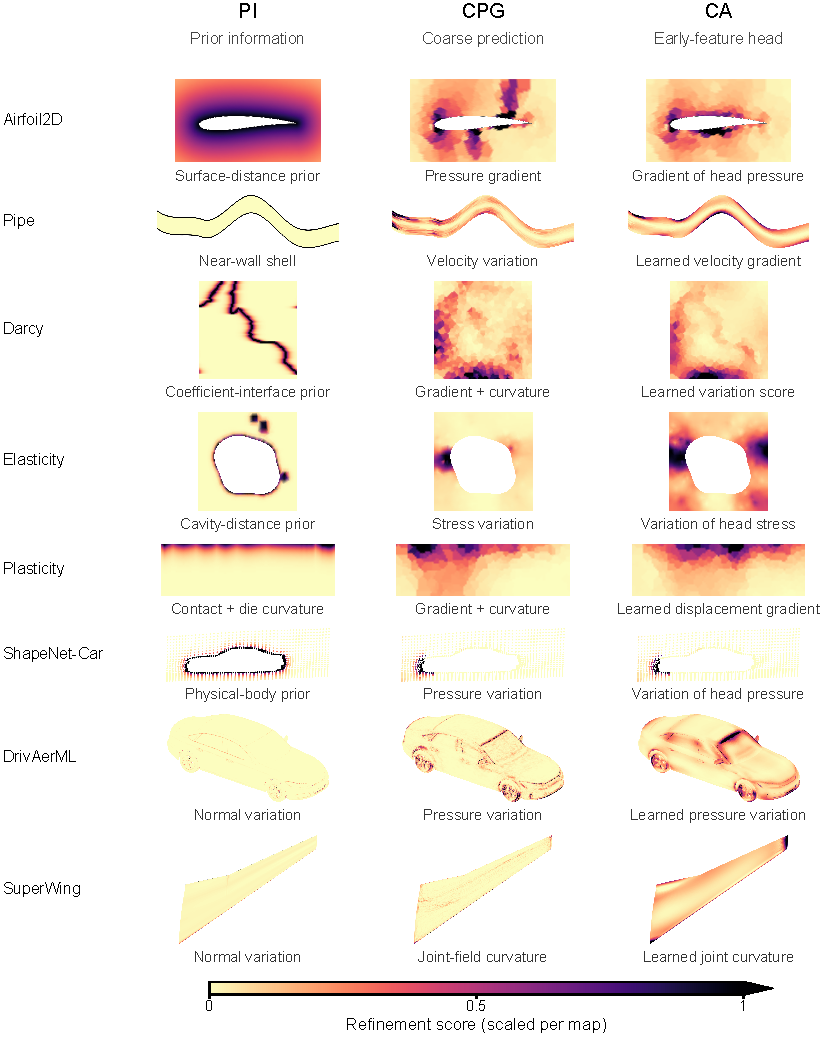
\includegraphics[width=\linewidth,height=.71\textheight,keepaspectratio]{figures/appendix/refinement_score_overview.pdf}
    \caption{\textbf{\DIFaddFL{Refinement scores.}} \DIFaddFL{Rows use the eight benchmark cases
    and views of the retained-fraction visualization at a $37.5\%$ budget
    and sampling seed zero. Each map is independently rescaled from its
    minimum to its 99th percentile, with larger values clipped to one.
    Colors progress from pale yellow to dark purple as the score increases.
    Labels identify each signal. Uniform has no refinement score.}}
    \label{fig:appendix_refinement_scores}
\end{figure}

\clearpage
\subsubsection{\DIFadd{From scores to selected points}}
\label{app:score_to_sampling}

\DIFadd{Figure~\ref{fig:refinement_score_example} traces one Airfoil case from
the available information through the raw score and sampling weights to
the selected points. Table~\ref{tab:airfoil_score_weights} specifies the
transformations. Here $d_\Gamma$ is the distance to the surface,
$x_{\mathrm{NN}}$ is the nearest coarse point, and $Q_{95}$ is the 95th
percentile over reference points.
}

\begin{table}[H]
    \centering
    \caption{\DIFaddFL{Raw scores and sampling weights for the Airfoil example.}}
    \label{tab:airfoil_score_weights}
    \small
    \renewcommand{\arraystretch}{1.25}
    \begin{tabular}{@{}lcc@{}}
        \toprule
        \DIFaddFL{Policy }& \DIFaddFL{Raw score $s(x)$ }& \DIFaddFL{Sampling weight $w(x)$ }\\
        \midrule
        \DIFaddFL{PI }& \DIFaddFL{$\exp(-d_\Gamma(x)/0.3)$ }& \DIFaddFL{$1+20s$ }\\
        \DIFaddFL{CPG }& \DIFaddFL{$\|\nabla_{\mathrm{LSQ},16}\widehat p^{(0)}(x_{\mathrm{NN}})\|_2$
            }& \DIFaddFL{$(0.1+s/Q_{95}(s))^2$ }\\
        \DIFaddFL{CA }& \DIFaddFL{$\|\nabla_{\mathrm{LSQ},16}\widehat p^{\mathrm{head}}(x_{\mathrm{NN}})\|_2$
            }& \DIFaddFL{$(0.01+s/Q_{95}(s))^2$ }\\
        \bottomrule
    \end{tabular}
\end{table}

\DIFadd{Sampling uses the raw scores and weights in
Table~\ref{tab:airfoil_score_weights}. The weights are normalized over
eligible candidates before sampling without replacement. Score colors
use the independent minimum-to-99th-percentile scaling of the overview.
}

\begin{figure}[H]
    \centering
    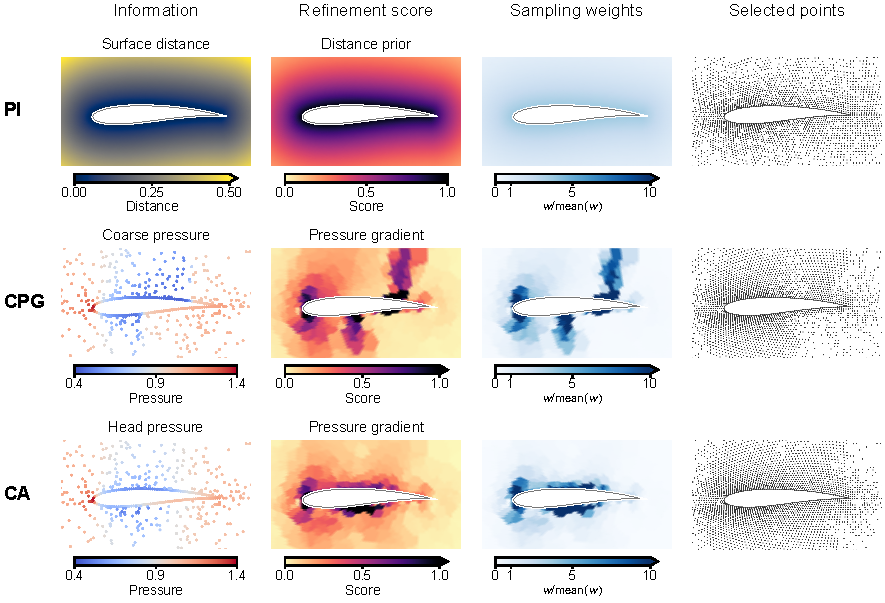
\includegraphics[width=\linewidth]{figures/appendix/refinement_score_example.pdf}
    \caption{\textbf{\DIFaddFL{How scores guide sampling.}} \DIFaddFL{Each row shows one policy
    on the same airfoil: input information, refinement score, sampling
    weights, and selected points. Table~\ref{tab:airfoil_score_weights}
    gives the raw-score definitions and sampling transformations.}}
    \label{fig:refinement_score_example}
\end{figure}


\DIFaddend \FloatBarrier
\DIFaddbegin \clearpage
\section{\DIFadd{Full-Field Reconstruction}}
\label{app:full_field_reconstruction}

\DIFadd{For full-field evaluation, we use piecewise-linear interpolation for Airfoil,
Pipe, Plasticity, SuperWing, Darcy, and Elasticity, with nearest-neighbor
assignment outside the convex hull of the retained points. ShapeNet-Car
uses four-neighbor inverse-distance interpolation, and DrivAerML uses
nearest-neighbor assignment. These procedures require neither ground-truth
fields nor an additional learned reconstruction model.
}

\section{\DIFadd{2-D Airfoil Inverse-Design Experiment}}
\label{app:airfoil_inverse_design_multiseed}

\DIFadd{Table~\ref{tab:airfoil_inverse_design_multiseed} reports multi-seed results
for the 2-D Airfoil inverse-design experiment from three initial geometries.
We compare the CFD-evaluated $C_D/C_L$ of designs obtained using full-mesh
inference, uniform sampling, and AdaSolver.
}

\begin{table}[!htbp]
    \centering
    \small
    \caption{\DIFaddFL{Multi-seed 2-D Airfoil inverse design. Lower CFD $C_D/C_L$ is better.
    Uniform and AdaSolver report mean $\pm$ standard deviation over three random
    seeds. Parentheses give the percentage change from the corresponding
    full-mesh result.}}
    \label{tab:airfoil_inverse_design_multiseed}
    \setlength{\tabcolsep}{3pt}
    \renewcommand{\arraystretch}{1.15}
    \begin{tabular*}{\textwidth}{@{\extracolsep{\fill}}cccc@{}}
        \toprule
        \DIFaddFL{\shortstack{Initial CFD\\$C_D/C_L$}
        }& \DIFaddFL{\shortstack{Full CFD\\$C_D/C_L$}
        }& \DIFaddFL{\shortstack{Uniform CFD\\$C_D/C_L$}
        }& \DIFaddFL{\shortstack{AdaSolver CFD\\$C_D/C_L$} }\\
        \midrule
        \DIFaddFL{$0.605367$ }& \DIFaddFL{$0.058752$
        }& \DIFaddFL{$0.060725\pm0.001814$ }& \DIFaddFL{$0.058621\pm0.000074$ }\\[1pt]
        & & \DIFaddFL{$(+3.36\%)$ }& \DIFaddFL{$(-0.22\%)$ }\\
        \addlinespace[4pt]
        \DIFaddFL{$0.246692$ }& \DIFaddFL{$0.058792$
        }& \DIFaddFL{$0.061417\pm0.000614$ }& \DIFaddFL{$0.058696\pm0.000164$ }\\[1pt]
        & & \DIFaddFL{$(+4.46\%)$ }& \DIFaddFL{$(-0.16\%)$ }\\
        \addlinespace[4pt]
        \DIFaddFL{$0.146587$ }& \DIFaddFL{$0.058748$
        }& \DIFaddFL{$0.061688\pm0.000117$ }& \DIFaddFL{$0.058601\pm0.000034$ }\\[1pt]
        & & \DIFaddFL{$(+5.00\%)$ }& \DIFaddFL{$(-0.25\%)$ }\\
        \bottomrule
    \end{tabular*}
\end{table}

\FloatBarrier

\DIFadd{Across these initial geometries, AdaSolver achieves better aerodynamic
performance on average and shorter optimization times than full-mesh
inference, whereas uniform sampling yields designs with poorer aerodynamic
performance.
}

\clearpage
\section{\DIFadd{Extending AdaSolver to LinearNO}}
\label{app:linearno_extension}

\DIFadd{We extend AdaSolver to LinearNO~\mbox{%DIFAUXCMD
\citep{hu2026transolverlinear} }\hspace{0pt}%DIFAUXCMD
to evaluate
adaptive sampling beyond the Transolver backbone.
}

\paragraph{\DIFadd{Spatial aggregation.}}
\DIFadd{For point features $H_N=[h_1,\ldots,h_N]^\top$, LinearNO computes
}\begin{equation}
    \DIFadd{\operatorname{LinearNO}(H_N)
    =\phi(Q)\bigl(\psi^\top(K)V_N\bigr),
    \qquad V_N=\operatorname{Linear}^{(V)}(H_N).
    \label{eq:linearno_original}
}\end{equation}
\DIFadd{The aggregation $\psi^\top(K)V_N$ uses a softmax over the spatial points.
Writing $\ell_{ij}=[\operatorname{Linear}^{(K)}(h_i)]_j$ and $v_i$ for the
value vector at point $i$, each aggregated representation is
}\begin{equation}
    \DIFadd{s_j=\frac{\sum_{i=1}^{N}\exp(\ell_{ij})v_i}{\sum_{i=1}^{N}\exp(\ell_{ij})}.
    \label{eq:linearno_aggregation}
}\end{equation}
\DIFadd{Changing the sampling measure from $\rho$ to $\widetilde\rho$ changes the
measure underlying this weighted average, even when the physical input
and model parameters remain fixed.
}

\paragraph{\DIFadd{Density correction.}}
\DIFadd{Using $c_i=(\mathrm{d}\rho/\mathrm{d}\widetilde\rho)(x_i)$ and
$\mathbf c=(c_1,\ldots,c_N)^\top$, we replace the aggregation by
}\begin{equation}
    \DIFadd{\widehat s_j
    =\frac{\sum_{i=1}^{N}c_i\exp(\ell_{ij})v_i}{\sum_{i=1}^{N}c_i\exp(\ell_{ij})}
    =\sum_{i=1}^{N}\left[
        \operatorname{Softmax}_{N}(\ell_{\cdot j}+\log\mathbf c)
      \right]_i v_i.
    \label{eq:linearno_corrected_aggregation}
}\end{equation}
\DIFadd{This correction adds $\log c_i$ to the key logits before the spatial
softmax. The complete module becomes
}\begin{equation}
    \DIFadd{\boxed{
    \operatorname{LinearNO}_{c}(H_N)
    =\phi(Q)\!\left[
      \operatorname{Softmax}_{N}\!\left(
        \operatorname{Linear}^{(K)}(H_N)^\top
        +\mathbf 1_M(\log\mathbf c)^\top
      \right)V_N
    \right].}
    \label{eq:linearno_corrected_module}
}\end{equation}
\DIFadd{Here, $M$ is the number of aggregation channels, $\mathbf 1_M$ is the
all-ones vector, and $\operatorname{Softmax}_{N}$ normalizes over the $N$
spatial points. We apply the correction at each spatial aggregation layer,
leaving the learned parameters and query-side normalization unchanged.
Under the usual support, integrability, and positive-denominator assumptions,
the corrected aggregation converges to its reference-measure counterpart.
}

\paragraph{\DIFadd{Airfoil and ShapeNet-Car results.}}
\DIFadd{Table~\ref{tab:linearno_airfoil} compares the two backbones on Airfoil field
prediction and on ShapeNet-Car field and drag-coefficient prediction.
All three policies improve on Uniform for both backbones across these
metrics, showing that the accuracy--point-budget benefits of adaptive
sampling extend to LinearNO.
}

\begin{table}[!htbp]
    \centering
    \small
    \caption{\DIFaddFL{Airfoil2D and ShapeNet-Car results for two backbones. Entries
    report mean $\pm$ standard deviation. Transolver results are taken from
    Tables~\ref{tab:standard_benchmarks} and~\ref{tab:industrial_benchmarks}.
    Uniform is normalized to $1$ for each backbone and metric. Lower is better.}}
    \label{tab:linearno_airfoil}
    \setlength{\tabcolsep}{3pt}
    \renewcommand{\arraystretch}{1.15}
    \begin{tabular*}{\textwidth}{@{\extracolsep{\fill}}lccc@{}}
        \toprule
        \DIFaddFL{Backbone }& \DIFaddFL{PI }& \DIFaddFL{CPG }& \DIFaddFL{CA }\\
        \midrule
        \multicolumn{4}{l}{\textbf{Airfoil2D: Field}} \\
        \addlinespace[2pt]
        \DIFaddFL{Transolver }& \DIFaddFL{$0.6166\pm0.0197$
        }& \DIFaddFL{$0.5831\pm0.0219$ }& \DIFaddFL{$0.5579\pm0.0139$ }\\
        \addlinespace[3pt]
        \DIFaddFL{LinearNO }& \DIFaddFL{$0.680622\pm0.030819$
        }& \DIFaddFL{$0.559296\pm0.021060$ }& \DIFaddFL{$0.589981\pm0.025945$ }\\
        \midrule
        \multicolumn{4}{l}{\textbf{ShapeNet-Car: Field}} \\
        \addlinespace[2pt]
        \DIFaddFL{Transolver }& \DIFaddFL{$0.49792\pm0.00163$
        }& \DIFaddFL{$0.50064\pm0.00157$ }& \DIFaddFL{$0.50063\pm0.00159$ }\\
        \addlinespace[3pt]
        \DIFaddFL{LinearNO }& \DIFaddFL{$0.574891\pm0.002469$
        }& \DIFaddFL{$0.531376\pm0.002579$ }& \DIFaddFL{$0.531345\pm0.002640$ }\\
        \midrule
        \multicolumn{4}{l}{\textbf{ShapeNet-Car: $C_D$}} \\
        \addlinespace[2pt]
        \DIFaddFL{Transolver }& \DIFaddFL{$0.63346\pm0.00328$
        }& \DIFaddFL{$0.63530\pm0.00396$ }& \DIFaddFL{$0.63540\pm0.00440$ }\\
        \addlinespace[3pt]
        \DIFaddFL{LinearNO }& \DIFaddFL{$0.596994\pm0.025766$
        }& \DIFaddFL{$0.604585\pm0.025192$ }& \DIFaddFL{$0.603715\pm0.024437$ }\\
        \bottomrule
    \end{tabular*}
\end{table}

\FloatBarrier

\DIFaddend \section*{Acknowledgements}

We used large language models to assist with literature discovery and to edit and polish the manuscript.
The authors checked the cited literature against the original sources and reviewed and revised the
AI-assisted edits. All final research and editorial decisions were made by the authors, who take full
responsibility for the content, accuracy, originality, and integrity of this work.

\clearpage
\begingroup
\centering
{\large\bfseries Figure change review 1}\par
{\small\path{figures/fig1_overview.pdf}}\par\medskip
{\color{red}\bfseries Baseline}\par\smallskip
\DIFOincludegraphics[width=\linewidth,height=.36\textheight,keepaspectratio]{review_assets/baseline/d4021228aa183f7d5f7912124d17d3f69f8930b9/figures/fig1_overview.pdf}\par\medskip
{\color{blue}\bfseries Current}\par\smallskip
\DIFOincludegraphics[width=\linewidth,height=.36\textheight,keepaspectratio]{figures/fig1_overview.pdf}\par
\endgroup

\clearpage
\begingroup
\centering
{\large\bfseries Figure change review 2}\par
{\small\path{figures/fig2_field_comparison.pdf}}\par\medskip
{\color{red}\bfseries Baseline}\par\smallskip
\DIFOincludegraphics[width=\linewidth,height=.36\textheight,keepaspectratio]{review_assets/baseline/d4021228aa183f7d5f7912124d17d3f69f8930b9/figures/fig2_field_comparison.pdf}\par\medskip
{\color{blue}\bfseries Current}\par\smallskip
\DIFOincludegraphics[width=\linewidth,height=.36\textheight,keepaspectratio]{figures/fig2_field_comparison.pdf}\par
\endgroup

\clearpage
\begingroup
\centering
{\large\bfseries Figure change review 3}\par
{\small\path{figures/fig3_airfoil_optimization.pdf}}\par\medskip
{\color{red}\bfseries Baseline}\par\smallskip
\DIFOincludegraphics[width=\linewidth,height=.36\textheight,keepaspectratio]{review_assets/baseline/d4021228aa183f7d5f7912124d17d3f69f8930b9/figures/fig3_airfoil_optimization.pdf}\par\medskip
{\color{blue}\bfseries Current}\par\smallskip
\DIFOincludegraphics[width=\linewidth,height=.36\textheight,keepaspectratio]{figures/fig3_airfoil_optimization.pdf}\par
\endgroup

\clearpage
\begingroup
\centering
{\large\bfseries Figure change review 4}\par
{\small\path{figures/fig4_superwing_optimization.pdf}}\par\medskip
{\color{red}\bfseries Baseline}\par\smallskip
\DIFOincludegraphics[width=\linewidth,height=.36\textheight,keepaspectratio]{review_assets/baseline/d4021228aa183f7d5f7912124d17d3f69f8930b9/figures/fig4_superwing_optimization.pdf}\par\medskip
{\color{blue}\bfseries Current}\par\smallskip
\DIFOincludegraphics[width=\linewidth,height=.36\textheight,keepaspectratio]{figures/fig4_superwing_optimization.pdf}\par
\endgroup

\clearpage
\begingroup
\centering
{\large\bfseries Figure change review 5}\par
{\small\path{figures/appendix/budget_error_curves.pdf}}\par\medskip
{\color{red}\bfseries Baseline}\par\smallskip
\DIFOincludegraphics[width=\linewidth,height=.36\textheight,keepaspectratio]{review_assets/baseline/d4021228aa183f7d5f7912124d17d3f69f8930b9/figures/appendix/budget_error_curves.pdf}\par\medskip
{\color{blue}\bfseries Current}\par\smallskip
\DIFOincludegraphics[width=\linewidth,height=.36\textheight,keepaspectratio]{figures/appendix/budget_error_curves.pdf}\par
\endgroup

\clearpage
\begingroup
\centering
{\large\bfseries Figure change review 6}\par
{\small\path{figures/appendix/elasticity_fields.pdf}}\par\medskip
{\color{red}\bfseries Baseline}\par\smallskip
\DIFOincludegraphics[width=\linewidth,height=.36\textheight,keepaspectratio]{review_assets/baseline/d4021228aa183f7d5f7912124d17d3f69f8930b9/figures/appendix/elasticity_fields.pdf}\par\medskip
{\color{blue}\bfseries Current}\par\smallskip
\DIFOincludegraphics[width=\linewidth,height=.36\textheight,keepaspectratio]{figures/appendix/elasticity_fields.pdf}\par
\endgroup

\clearpage
\begingroup
\centering
{\large\bfseries Figure change review 7}\par
{\small\path{figures/appendix/beta_ablation.pdf}}\par\medskip
{\color{red}\bfseries Baseline}\par\smallskip
\DIFOincludegraphics[width=\linewidth,height=.36\textheight,keepaspectratio]{review_assets/baseline/d4021228aa183f7d5f7912124d17d3f69f8930b9/figures/appendix/beta_ablation.pdf}\par\medskip
{\color{blue}\bfseries Current}\par\smallskip
\DIFOincludegraphics[width=\linewidth,height=.36\textheight,keepaspectratio]{figures/appendix/beta_ablation.pdf}\par
\endgroup
\end{document}
